\documentclass{article}
\usepackage[a4paper, margin=2.5cm]{geometry}
\usepackage[utf8]{inputenc}
\usepackage[shortlabels]{enumitem}
\usepackage{graphicx, wrapfig, float, xcolor, hyperref, subfiles, bigints, eurosym, amsfonts}
\usepackage[makeroom]{cancel}
\usepackage{bigints}


\title{Natuurkunde II - OZ oplossingen}
\author{Jonas Couwberghs, Pieter Vanderschueren}
\date{2023-2024}

% section titles niet tonen voor schoonheid
\newcommand{\fakesection}[1]{
  \par\refstepcounter{section}
  \sectionmark{#1}
  \addcontentsline{toc}{section}{\protect\numberline{\thesection}#1}
}

\newcommand{\fakesubsection}[1]{
  \par\refstepcounter{subsection}
  \subsectionmark{#1}
  \addcontentsline{toc}{subsection}{\protect\numberline{\thesubsection}#1}
}

\counterwithin*{equation}{section}% Reset equation at \section
\counterwithin*{equation}{subsection}% Reset equation at \subsection
\counterwithin*{equation}{subsubsection}% Reset equation at \subsubsection

\begin{document}
\setlength{\parindent}{0cm}

\maketitle

\begin{description}[labelwidth=1.4cm, leftmargin=!]
    \item[\textcolor{red}{Rood:}] Uitwerking nog niet af
    \item[\textcolor{orange}{Oranje:}] Niet zeker of de uitwerking correct is
    \item[\textcolor{yellow}{Geel:}] Uitwerking gekopieerd uit handboek
\end{description}

\begin{description}[labelwidth=0.5cm, leftmargin=!]
    \item[\hyperlink{section.1}{Oefenzitting 1:}] \leavevmode
        \begin{description}
            \item[\hyperlink{subsection.1.1}{Herhaling}]
                \hyperref[OZ1:herhaling:1]{Oef 1}
                \hyperref[OZ1:herhaling:2]{Oef 2}
                \hyperref[OZ1:herhaling:3]{Oef 3}
                \hyperref[OZ1:herhaling:4]{Oef 4}
            \item[\hyperlink{subsection.1.2}{Magnetische velden voor beginners}]
                \hyperref[OZ1:velden:1]{Oef 1}
                \hyperref[OZ1:velden:2]{Oef 2}
        \end{description}
        
    \item[\hyperlink{section.2}{Oefenzitting 2:}] \leavevmode
        \begin{description}
            \item
                \hyperref[OZ2:1]{Oef 1}
                \hyperref[OZ2:2]{Oef 2}
                \hyperref[OZ2:3]{Oef 3}
                \hyperref[OZ2:4]{{Oef 4}}
                \hyperref[OZ2:5]{Oef 5}
        \end{description}
    
    \item[\hyperlink{section.3}{Oefenzitting 3:}] \leavevmode
        \begin{description}
            \item
            % [\hyperlink{subsection.3.1}{De Lorentzkracht en de wet van Ampère}]
                \hyperref[OZ3:1]{Oef 1}
                \hyperref[OZ3:2]{Oef 2}
                \hyperref[OZ3:3]{Oef 3}
                \hyperref[OZ3:4]{Oef 4}
                \hyperref[OZ3:5]{Oef 5}
        \end{description}
        
    \item[\hyperlink{section.4}{Oefenzitting 4:}] \leavevmode
        \begin{description}
            \item
            % [\hyperlink{subsection.4.1}{De wet van Ampère en de wet van Biot-Savart}]
                \hyperref[OZ4:1]{Oef 1}
                \hyperref[OZ4:2]{Oef 2}
                \hyperref[OZ4:3]{Oef 3}
                \hyperref[OZ4:4]{Oef 4}
                \hyperref[OZ4:5]{Oef 5}
        \end{description}
        
    \item[\hyperlink{section.5}{Oefenzitting 5:}] \leavevmode
        \begin{description}
            \item
            % [\hyperlink{subsection.5.1}{Magnetische inductie en de wet van Faraday}]
                \hyperref[OZ5:1]{Oef 1}
                \hyperref[OZ5:2]{Oef 2}
                \hyperref[OZ5:3]{Oef 3}
                \hyperref[OZ5:4]{Oef 4}
                \hyperref[OZ5:5]{Oef 5}
        \end{description}
        
    \item[\hyperlink{section.6}{Oefenzitting 6:}] \leavevmode
        \begin{description}
            \item
            % [\hyperlink{subsection.6.1}{Magnetische inductie en de wet van Faraday}]
                \hyperref[OZ6:1]{Oef 1}
                \hyperref[OZ6:2]{Oef 2}
                \hyperref[OZ6:3]{Oef 3}
                \hyperref[OZ6:4]{Oef 4}
                \hyperref[OZ6:5]{Oef 5}
        \end{description}
        
    \item[\hyperlink{section.7}{Oefenzitting 7:}] \leavevmode
        \begin{description}
            \item
            % [\hyperlink{subsection.7.1}{Inductantie}]
                \hyperref[OZ7:1]{Oef 1}
                \hyperref[OZ7:2]{Oef 2}
                \hyperref[OZ7:3]{Oef 3}
                \hyperref[OZ7:4]{Oef 4}
                \hyperref[OZ7:5]{Oef 5}
        \end{description}
        
    \item[\hyperlink{section.8}{Oefenzitting 8:}] \leavevmode
        \begin{description}
            \item
            % [\hyperlink{subsection.8.1}{$ LC $- en $ RLC $-circuits}]
                \hyperref[OZ8:1]{Oef 1}
                \hyperref[OZ8:2]{Oef 2}
                \hyperref[OZ8:3]{Oef 3}
                \hyperref[OZ8:4]{Oef 4}
                \hyperref[OZ8:5]{Oef 5}
        \end{description}
        
    \item[\hyperlink{section.9}{Oefenzitting 9:}] \leavevmode
        \begin{description}
            \item
            % [\hyperlink{subsection.9.1}{Wisselstroomkringen}]
                \hyperref[OZ9:1]{Oef 1}
                \hyperref[OZ9:2]{Oef 2}
                \hyperref[OZ9:3]{Oef 3}
                \hyperref[OZ9:4]{Oef 4}
                \hyperref[OZ9:5]{Oef 5}
        \end{description}
        
    \item[\hyperlink{section.10}{Oefenzitting 10:}] \leavevmode
        \begin{description}
            \item
            % [\hyperlink{subsection.10.1}{De vergelijkingen van Maxwell + Herhaling}]
                \hyperref[OZ10:1]{Oef 1}
                \hyperref[OZ10:2]{Oef 2}
                \hyperref[OZ10:3]{Oef 3}
                \hyperref[OZ10:4]{Oef 4}
                \hyperref[OZ10:5]{Oef 5}
                \hyperref[OZ10:6]{Oef 6}
        \end{description}
\end{description}

\pagebreak

\fakesection{Oefenzitting 1}

\fakesubsection{Herhaling}

\phantomsection
\label{OZ1:herhaling:1}
\textbf{\underline{OZ 1 - Herhaling - Oefening 1:}}
\vspace{0.5cm}

Bereken de volgende \textbf{vectorproducten}:

\begin{enumerate}[(a)]
    \item 
        $ \hat{j} \times \hat{i} $  
    
          \hspace{0.5cm} $ = -(\hat{i} \times \hat{j}) $

          \hspace{0.5cm} $ = -\hat{k} $
    
    \item $ \left( \hat{j} \times \hat{k} \right) \times \hat{j} $
    
          \hspace{0.5cm} $ = \left( \left( 0, 1, 0 \right) \times \left( 0, 0, 1 \right) \right) \times \hat{j} $
    
          \hspace{0.5cm} $ = \left( 1, 0, 0 \right) \times \hat{j} $
    
          \hspace{0.5cm} $ = \hat{i} \times \hat{j} $
    
          \hspace{0.5cm} $ = \hat{k} $
    
    \item $ \hat{j} \times \left( \hat{j} \times \hat{k} \right) $
    
          \hspace{0.5cm} $ = \hat{j} \times \hat{i} $
    
          \hspace{0.5cm} $ = -(\hat{i} \times \hat{j})$
    
          \hspace{0.5cm} $ = -\hat{k} $
    
    \item $ (\hat{j} \times \hat{k}) \cdot (\hat{k} \times (\hat{k} \times \hat{i}) + (\hat{j} \times \hat{k}) \times \hat{j})) $

          \hspace{0.5cm} $ = \hat{i} \cdot (\hat{k} \times \hat{j} + \hat{i} \times \hat{j}) $

          \hspace{0.5cm} $ = \hat{i} \cdot ((-\hat{i}) + \hat{k}) $

          \hspace{0.5cm} $ = (1,0,0) \cdot (-1,0,1) $

          \hspace{0.5cm} $ = -1 $
\end{enumerate}

\vspace{1cm}

\phantomsection
\label{OZ1:herhaling:2}
\textbf{\underline{OZ 1 - Herhaling - Oefening 2:}}
\vspace{0.5cm}

Alvorens de reus Goliath te verslaan door een steen tegen zijn kop te slingeren,
had David uiteraard eerst uitgetest welke lengte van slinger het meest effectief zou zijn. Zo bleek
dat hij een slinger van $r = 0,600$ m $8,00$ keer per seconde kon ronddraaien. Gebruikte hij een
slinger van $r = 0,900$ m, dan kreeg hij de slinger maar $6,00$ keer per seconde rondgedraaid (neem
aan dat de steen in de slinger in beide gevallen dezelfde is).

\begin{enumerate}[(a)]
    \item Welke slingerlengte is het meest effectief? (Anders geformuleerd: welke slinger zorgt voor de grootste snelheid van de steen?)
    \item Wat is de centripetale versnelling van de steen in beide gevallen?
    \item Levert David arbeid bij het ronddraaien van de slinger?
\end{enumerate}

\begin{enumerate}[(a)]
    \item 
        \begin{description}[labelwidth=1.5cm, leftmargin=!]
            \item[Geg. :]  $r_{1} = 0.600$m, $f_{1} = 8.00$Hz  $r_{2} = 0.900$m, $f_{2} = 6.00$Hz
            \item[Gevr. :] $v_{1}, v_{2}$?
            \item[Opl. :]  
                $v_{1} = \omega_{1} r_{1} = 2 \pi f_{1} r_{1} = 2\pi(0.600)(8.00) \approx 30.2 \text{m/s}\\$
                \hspace{0.5cm}$v_{2} = \omega_{1} r_{1} = 2 \pi f_{2} r_{2} = 2\pi(0.900)(6.00) \approx 33.9 \text{m/s} \xleftarrow{} \text{sneller}$
        \end{description}
    \item 
        \begin{description}[labelwidth=1.5cm, leftmargin=!]
            \item[Geg. :]   $r_{1} = 0.600$m, $v_{1} = 30.2$m/s  $r_{2} = 0.900$m, $v_{2} = 33.9$Hz
            \item[Gevr. :]  $a_{R,1}, a_{R,2}$
            \item[Opl. :]   
                $a_{R,1} = \dfrac{v_{1}^2}{r_{1}} = \dfrac{(30.2)^2}{0.600} \approx 1.52$km/s$^2$ \vspace{0.2cm}\\
                \hspace{0.5cm} $a_{R,2} = \dfrac{v_{2}^2}{r_{2}} = \dfrac{(33.9)^2}{0.900} \approx 1.28$km/s$^2$
        \end{description}
    \item 
        \begin{description}[labelwidth=1.5cm, leftmargin=!]
            \item[Gevr. :]  Levert David arbeid?
            \item[Opl. :]   Ja, Dabid levert arbeid bij het ronddraien van de slinger. David voert een kracht uit op de steen waardoor deze rotationeel versneld; hij levert dus arbeid op de steen.
        \end{description}
\end{enumerate}


\phantomsection
\label{OZ1:herhaling:3}
\textbf{\underline{OZ 1 - Herhaling - Oefening 3:}}
\vspace{0.5cm}

Een klein rigide object draagt een positieve lading en een negatieve lading van $3,50 $nC. De oriëntatie van het object is zo dat de positieve lading zich op ($-1,20 $mm,
$1,10 $mm) bevindt en de negatieve lading op ($1,40 $mm, $-1,30$ mm). Het object wordt geplaatst in
een elektrisch veld $\Vec{E} = (7800\hat{i} - 4900\hat{j})$ N/C.

\begin{enumerate}[(a)]
    \item Wat is het elektrisch dipoolmoment van het object?
    \item Wat is de torsie die het elektrisch veld op het object uitoefent?
    \item Wat is de potentiële energie van het object-veld systeem als het object in deze oriëntatie blijft?
    \item Als je aanneemt dat de oriëntatie van het object kan veranderen, wat is het verschil tussen maximum en minimum potentiële energie van het systeem?
\end{enumerate}

% \begin{description}[labelwidth=1.5cm, leftmargin=!]
%     \item[Geg. :]  
%     \item[Gevr. :]  
%     \item[Opl. :]   
% \end{description}

\begin{enumerate}[(a)]
    \item 
        \begin{description}[labelwidth=1.5cm, leftmargin=!]
            \item[Geg. :]  $q = -3.50$nC, $\Vec{r}_{+} = (-1.20\text{mm}, 1.10\text{mm})$, $\Vec{r}_{-} = (1.40\text{mm}, -1.30\text{mm})$
            \item[Gevr. :] $\Vec{p}$ ?
            \item[Opl. :]  $\Vec{p} = q\Vec{\ell} = q(\Vec{r}_{-} - \Vec{r}_{+}) 
                                  % = q((1.40\hat{i} - 1.30\hat{j}) - (-1.20\hat{i} + 1.10\hat{j})) 
                                    = q(2.60\hat{i} + - 2.40\hat{j}) \approx (-9.10\hat{i} + 8.40\hat{j}) \cdot 10^{-12}$ Cm
        \end{description}
        
    \item 
        \begin{description}[labelwidth=1.5cm, leftmargin=!]
            \item[Geg. :]  $\Vec{p} = (-9.10\hat{i} + 8.40\hat{j}) \cdot 10^{-12}$ Cm, $\Vec{E} = (7800\hat{i} - 4900\hat{j})$ N/C
            \item[Gevr. :] $\Vec{\tau}$ ?
            \item[Opl. :]  $\Vec{\tau} = \Vec{p} \times \Vec{E} = 
                            \begin{vmatrix}
                                \hat{i} & \hat{j} & \hat{k}\\ 
                                p_x & p_y & p_z\\
                                E_x & E_y & E_z  
                            \end{vmatrix} 
                            = 
                            \begin{vmatrix}
                                \hat{i} & \hat{j} & \hat{k}\\ 
                                -9.10 \cdot 10^{-12} & 8.40 \cdot 10^{-12} & 0\\
                                7800 & -4900 & 0  
                            \end{vmatrix} 
                            % =
                            % \begin{vmatrix}
                            %     -9.10 \cdot 10^{-12} & 8.40 \cdot 10^{-12}\\
                            %     7800 & -4900
                            % \end{vmatrix}\hat{k}
                            \approx -2.09 \cdot 10^{-8} \text{ Nm } \hat{k}$
        \end{description}
        
    \item 
        \begin{description}[labelwidth=1.5cm, leftmargin=!]
            \item[Geg. :]  $\Vec{p} = (-9.10\hat{i} + 8.40\hat{j}) \cdot 10^{-12}$ Cm, $\Vec{E} = (7800\hat{i} - 4900\hat{j})$ N/C
            \item[Gevr. :]  $U$?
            \item[Opl. :]   $U = -\Vec{p} \cdot \Vec{E} = -\sum_{i=1}^n p_iE_i \approx 1.12 \cdot 10^{-7}$Nm 
        \end{description}

    \item 
        \begin{description}[labelwidth=1.5cm, leftmargin=!]
            \item[Geg. :]  $\Vec{p} = (-9.10\hat{i} + 8.40\hat{j}) \cdot 10^{-12}$ Cm, $\Vec{E} = (7800\hat{i} - 4900\hat{j})$ N/C
            \item[Gevr. :]  $\Delta U$ ?
            \item[Opl. :]   $U_{\text{max}} = -pE\cos(0^{\circ}) = - pE$ \\
                            \hspace{0.5cm}$U_{\text{min}} = -pE\cos(180^{\circ}) = pE$ \\ 
                            \hspace{0.5cm}$\Delta U = U_{\text{max}} - U_{\text{min}} = -2pE \approx 2.28 \cdot 10^{-7}$Nm
        \end{description}

\end{enumerate}

\newpage

\phantomsection
\label{OZ1:herhaling:4}
\textbf{\underline{OZ 1 - Herhaling - Oefening 4:}}
\vspace{0.5cm}


\begin{minipage}{.73\textwidth}
    Protonen worden met een snelheid $v_i = 9, 55 \text{km/s}$ in een regio
    met een uniform elektrische veld $\Vec{E} = -720\hat{k} \text{N/C}$ geschoten (zie figuur). Het is de bedoeling dat de protonenstraal een doelwit raakt dat zich $R = 1, 27 $ mm van het punt bevindt waar de
    straal het elektrisch veld binnenkomt. Bereken onder welke twee hoeken $\theta$ de protonenstraal het
    doelwit raakt en hoe lang de protonen zich boven het vlak in de tekening bevinden. (Verwaarloos
    de zwaartekracht, de massa van een proton is immers $1, 67E-27 $ kg).
\end{minipage}
\begin{minipage}{.23\textwidth}
    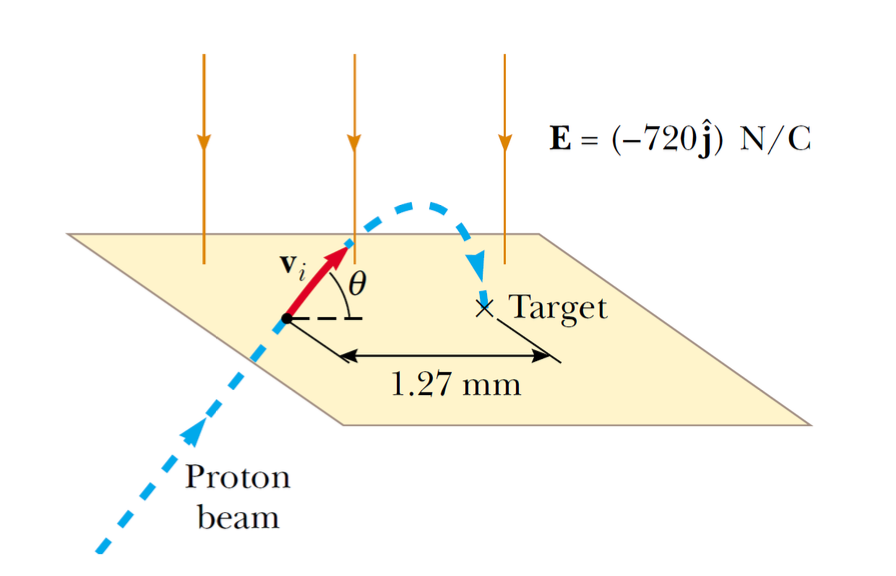
\includegraphics[scale = 0.31]{oz01/herhaling/resources/ElektronenElektrischVeld.png}
\end{minipage}

% \begin{description}[labelwidth=1.5cm, leftmargin=!]
%     \item[Geg. :]  
%     \item[Gevr. :]  
%     \item[Opl. :]   
% \end{description}

\begin{description}[labelwidth=1.5cm, leftmargin=!]
    \item[Geg. :]   $v_i = 9, 55 \text{km/s}$, $\Vec{E} = -720\hat{k} \text{N/C}$, $R = 1, 27 $ mm, $m_p = 1, 67E-27$ kg, $q = q_p$
    \item[Gevr. :]  $\theta$ ?
    \item[Opl. :]  
    \item[]
        \vspace{-0.7cm}
        \begin{minipage}{0.65\textwidth}
            Een lading in een elektrisch veld ondervindt een elektrische kracht, namelijk
            \begin{equation*}
                \Vec{F}_e = q_p\Vec{E}
            \end{equation*}
            waarbij parallel aan het veld is. We vinden door de tweede wet van Newton dat
            \begin{equation*}
                \Vec{a} = \frac{q_p}{m_p}\Vec{E}
            \end{equation*}
            waardoor deze oefening trivialiseert tot een projectielbeweging oefening. Neem het punt waar de protonen doorvliegen als de oorsprong.
        \end{minipage}
        \hspace{0.5cm}\begin{minipage}{.31\textwidth}
            \begin{center}
                \def\arraystretch{2}
                \begin{tabular}{c|c|c}
                     & $x$ & $y$ \\ \hline
                     $ r $ & $  v_i\cos(\theta)t $ & $  v_i\sin(\theta) - \frac{at^2}{2} $ \\ \hline
                     $ v $ & $ v_i\cos(\theta) $ & $ v_i\sin(\theta) - at $  \\ \hline
                     $ a $ & $ 0 $ & $ -a $ 
                \end{tabular}
            \end{center}
        \end{minipage}
    
        Stel $v_y$ de verticale snelheid op het hoogste punt, dan
        \begin{equation*}
            \frac{v_y-v_{0,y}}{a_y} = t
        \end{equation*}
        ofwel
        \begin{equation*}
            \frac{2v_i\sin(\theta)}{a_y} = t
        \end{equation*}
        waarbij we maal twee doen om een vergelijking te hebben voor heel de beweging, want het maxima komt voor in het midden van de beweging. We weten voor de x-as dat
        \begin{align*}
            R_x 
                &= v_i\cos(\theta)t \\
                &= v_i\cos(\theta)\left( \frac{2v_i\sin(\theta)}{a_y}\right) \\
                &=  \frac{v_i^2}{a_y} \sin(2\theta)
        \end{align*}
        wat we kunnen herwerken tot $\theta$
        \begin{equation*}
            \theta = \frac{1}{2}\sin^{-1}\left(\frac{a_yR_x}{v_i^2} \right) = 36.9^{\circ} \ \text{en} \ 53.1^{\circ} 
        \end{equation*}
        wat we kunnen invullen in de verticale snelheidsvergelijking om de volgende tijden te krijgen
        \begin{equation*}
            t_{36.9^{\circ}} = 1.66 \cdot 10^{-7} \text{ s} \ \text{en} \ t_{53.1^{\circ}} = 2.21 \cdot 10^{-7} \text{ s}
        \end{equation*}
        
    
\end{description}


\newpage

\fakesubsection{Magnetische velden voor beginners}

\phantomsection
\label{OZ1:velden:1}
\textbf{\underline{OZ 1 - Magnetische velden voor beginners - Oefening 1:}}
\vspace{0.5cm}

\textbf{Proton in magneetveld:} Een proton met een snelheid $ 4,00 \cdot 10^{6} $ m/s beweegt door een magneetveld van $ 1,70 T $ en ondergaat daardoor een kracht van $ 8,20 \cdot 10^{-13} N $. Wat is de hoek tussen het magnetische veld en de snelheidsvector van het proton?

\begin{description}[labelwidth=1.5cm, leftmargin=!]
    \item[Geg. :]   $ q = 1,60 \cdot 10^{-19} $ C; $ v = 4 \cdot 10^{6} $ m/s; $ B = 1,70 $ T; $ F = 8,20 \cdot 10^{-13} $ N;
    \item[Gevr. :]  $ \theta $;
    \item[Opl. :]   $ \vec{F} = q \vec{v} \times \vec{B} $
    
                    \hspace{-0.58cm} $ \Rightarrow
                    F = q v B \sin{\theta} $
    
                    \hspace{-0.58cm} $ \Leftrightarrow
                    \theta = \arcsin{\frac{F}{q v B}} $
                    
                    \hspace{0.12cm} $
                    = \arcsin{\frac{8,20 \cdot 10^{-13}}{1,60 \cdot 10^{-19} \cdot 4 \cdot 10^6 \cdot 1,70}} $
                    
                    \hspace{0.12cm} $
                    = 48,91^{\circ} \approx 48,9^{\circ} $
\end{description}

\vspace{1cm}

\phantomsection
\label{OZ1:velden:2}
\textbf{\underline{OZ 1 - Magnetische velden voor beginners - Oefening 2:}}
\vspace{0.5cm}

\textbf{Magnetische kracht op een stroomvoerende geleider:} Beeld je in dat er een stroomvoerende draad met dichtheid $ 2,40 $ g/m rond de aarde is gespannen ter hoogte van de (magnetische) evenaar. Neem aan dat het aardmagnetische veld daar een constante grootte heeft van $ 28,0 \ \mu$T, parallel is  met het aardoppervlak en wijst naar het noorden. Welke stroom (grootte en richting) moet er door de draad gestuurd worden om er voor te zorgen dat de draad blijft leviteren net boven de grond?

\begin{description}[labelwidth=1.5cm, leftmargin=!]
    \item[Geg. :]   $ \frac{dm}{ds} = 2,40 $ g/m $ = 2,40 \cdot 10^{-3} $ kg/m; $ 28,0 \ \mu$T; $ \theta = 90^{\circ} $;
    \item[Gevr. :]  $ \vec{I} $;
    \item[Opl. :]   $ d\vec{F} = I d\vec{s} \times \vec{B} $
    
                    \hspace{-0.58cm} $ \Leftrightarrow
                    dm \cdot g = I \cdot ds \cdot B \cdot \sin{90^{\circ}} $
    
                    \hspace{-0.58cm} $ \Leftrightarrow
                    I = \frac{dm \cdot g}{ds \cdot B \cdot \sin{90^{\circ}}} $
    
                    \hspace{0.13cm} $
                    = \frac{2,40 \cdot 10^{-3} \cdot 9,81}{28 \cdot 10^{-6} \cdot \sin{90^{\circ}}} $
    
                    \hspace{0.13cm} $
                    = 840,85714 $ A $ \approx 841 $ A;
\end{description}

\vspace{1cm}

\newpage

\newpage

\pagebreak

\fakesection{Oefenzitting 2}

\phantomsection
\label{OZ2:1}
\textbf{\underline{OZ 2 - Magnetische velden - Oefening 1:}}
\vspace{0.5cm}

Beschouw een massa separator met $E = 2, 48 \cdot 10^{4} $V/m en $B_{\text{in}} = B_{0,\text{in}} = 0,680 $T. We sturen nu koolstofionen met massagetallen 12, 13 en 14 door deze massa separator. Hoe ver liggen de lijnen van de verschillende (enkel geladen) isotopen uit elkaar op de detector? Wat als de ionen 2+ geladen zijn?

\begin{description}[labelwidth=1.5cm, leftmargin=!]
    \item[Geg. :]   $E = 2, 48 \cdot 10^{4} $ V/m, $B_{\text{in}} =         B_{0,\text{in}} = 0,680 $T, $ m_{1} = 12(1.67 \cdot 10^{-27})$ kg,
                    $ m_{2} = 13(1.67 \cdot 10^{-27})$ kg,
                    $ m_{3} = 14(1.67 \cdot 10^{-27})$ kg,
                    $q = 1.60 \cdot 10^{-19}$C
    \item[Gevr. :]  $d_{1 \to 2}, d_{2 \to 3}, d_{3 \to 1}$
    \item[Opl. :]  
                    $r_{1} = \dfrac{m_{1}v_{1}}{qB_{0,\text{in}}} =  \dfrac{m_{1}E}{qB_{\text{in}}B_{0,\text{in}}} = 6.67 \cdot 10^{-3}$ \vspace{0.3cm}\\
                    \hspace{0.57cm} $r_{2} = \dfrac{m_{2}v_{2}}{qB_{0,\text{in}}} =  \dfrac{m_{2}E}{qB_{\text{in}}B_{0,\text{in}}} = 7.23 \cdot 10^{-3}$ 
                    \vspace{0.3cm}\\
                    \hspace{0.57cm} $r_{3} = \dfrac{m_{3}v_{3}}{qB_{0,\text{in}}} =  \dfrac{m_{2}E}{qB_{\text{in}}B_{0,\text{in}}} = 7.79 \cdot 10^{-3}$ 
                    \vspace{0.3cm}\\
                    \hspace{0.57cm} $d_{1 \to 2} = 2r_{2} - 2r_{1} = 1.10 \cdot 10^{-3} $ 
                    \vspace{0.3cm}\\
                    \hspace{0.57cm} $d_{2 \to 3} = 2r_{3} - 2r_{2} = 1.12 \cdot 10^{-3} $ 
                    \vspace{0.3cm}\\
                    \hspace{0.57cm} $d_{3 \to 1} = 2r_{3} - 2r_{1} = 2.22 \cdot 10^{-3} $ 
                    \vspace{0.3cm}\\
                    Als we nu de lading 2 keer vergroten, dan zien we dat de straal 2 keer verkleint en dus halveert het verschilt tussen de lijnen. 

\end{description}

\vspace{1cm}

\phantomsection
\label{OZ2:2}
\textbf{\underline{OZ 2 - Magnetische velden - Oefening 2:}}
\vspace{0.5cm}

Een uniform magnetisch veld van $ 0,150 $ T ligt volgens de x-as. Een positron vliegt dit veld binnen met een snelheid van $5, 00 \cdot 10^6 $ m/s onder een hoek van $85,0^{\circ}$ met de x-as (de massa van een positron is $9, 11 \cdot 10^{-31} $ kg). Bereken de straal van de helix die
het positron gaat maken en ook de afstand p tussen twee opeenvolgende windingen van de helix.

% \begin{description}[labelwidth=1.5cm, leftmargin=!]
%     \item[Geg. :]   
%     \item[Gevr. :]  
%     \item[Opl. :]  
% \end{description}

\begin{description}[labelwidth=1.5cm, leftmargin=!]
    \item[Geg. :]   $ B = 0,150 $ T ,
                    $ v = 5, 00 \cdot 10^6 $ m/s,
                    $ \theta = 85,0^{\circ} $,
                    $ m = 9, 11 \cdot 10^{-31} $ kg                 
    \item[Gevr. :]  $ r, p$
    \item[Opl. :]   $ F_{B} = qvB\sin(\theta) = 1.20 \cdot 10^{-13} $ 
                    \vspace{0.3cm}\\ 
                    \hspace{-0.57cm} $ a_{R} = \dfrac{F_{B}}{m} = \dfrac{v^2}{r}$ \vspace{0.3cm}\\ 
                    \hspace{-0.57cm} $ r = \dfrac{mv^2}{F_{B}} = 1.89 \cdot 10^{-4}$
                    \vspace{0.3cm}\\ 
                    \hspace{-0.57cm} $ p = 2\pi r \cos(85^{\circ}) = 1.04 \cdot 10^{-4}$
                    
\end{description}

\vspace{1cm}

\newpage

\phantomsection
\label{OZ2:3}
\textbf{\underline{OZ 2 - Magnetische velden - Oefening 3:}}
\vspace{0.5cm}

% \begin{description}[labelwidth=1.5cm, leftmargin=!]
%     \item[Geg. :]   
%     \item[Gevr. :]  
%     \item[Opl. :]  
% \end{description}
Een stroom $I$ vloeit door een rechthoekige balk van geleidend materiaal terwijl een magnetisch veld $\Vec{B}$ is aangelegd zoals in de figuur. 

\begin{enumerate}[(a)]
    \item Als de ladingsdragers \textbf{positief} zijn, in welke richting worden ze dan afgebogen door het magnetisch veld? Deze afbuiging zorgt ervoor dat de bovenkant en de onderkant van de balk een netto lading krijgen. Dit produceert een elektrisch veld dat het effect van de magnetische kracht gaat tegenwerken. Het systeem is in evenwicht als de twee krachten elkaar opheffen.
    \item Wat is het potentiaalverschil tussen de boven- en onderkant van de balk als het systeem in evenwicht is? Druk je resultaat uit in functie van $B$, $v$ (de snelheid van de ladingsdragers) en de relevante afmetingen van de balk. (Vermeld ook welke kant de hoogste potentiaal heeft.)
    \item Wat zou er veranderen aan je antwoorden als de ladingsdragers negatief zouden zijn maar de stroom nog steeds in dezelfde richting zou lopen?
\end{enumerate}

\begin{enumerate}[(a)]
    \item Het zou uit het blad bewegen.
    \item 
        \begin{description}[labelwidth=1.5cm, leftmargin=!]
        \item[Gevr. :]  $\mathcal{E}_{H}$
        \item[Opl. :]   $\mathcal{E}_{H} = E_Hd = vBd $
        \end{description}
    \item De Hallspanning zou gelijk zijn, maar de ladingen zouden in het blad bewegen.
\end{enumerate}

\vspace{1cm}

\phantomsection
\label{OZ2:4}
\textbf{\underline{OZ 2 - Magnetische velden - Oefening 4:}}
\vspace{0.5cm}

Een draad van 4,00 m met massa 0,100 kg wordt gebruikt om een vierkante spoel met zijde 0,100 m te maken. De spoel wordt opgehangen aan ëën van zijn horizontale zijden in een verticaal magnetisch veld van 0,0100 T. Vervolgens stuurt men een stroom van 3,40 A door de spoel. Bepaal de hoek die de spoel maakt met de verticale wanneer de spoel zijn evenwichtspositie heeft bereikt. Wat is het krachtmoment (torsie) die het magnetisch veld op de spoel uitoefent in deze situatie?

\begin{description}[labelwidth=1.5cm, leftmargin=!]
    \item[Geg. :]   $ l = 4,00 $ m; $ m = 0,100 $ kg; $ z = 0,100 $ m; $ B = 0,0100 $ T; $ I = 3,40 $ A;
        % \begin{figure}[H]
        %     \centering
        %     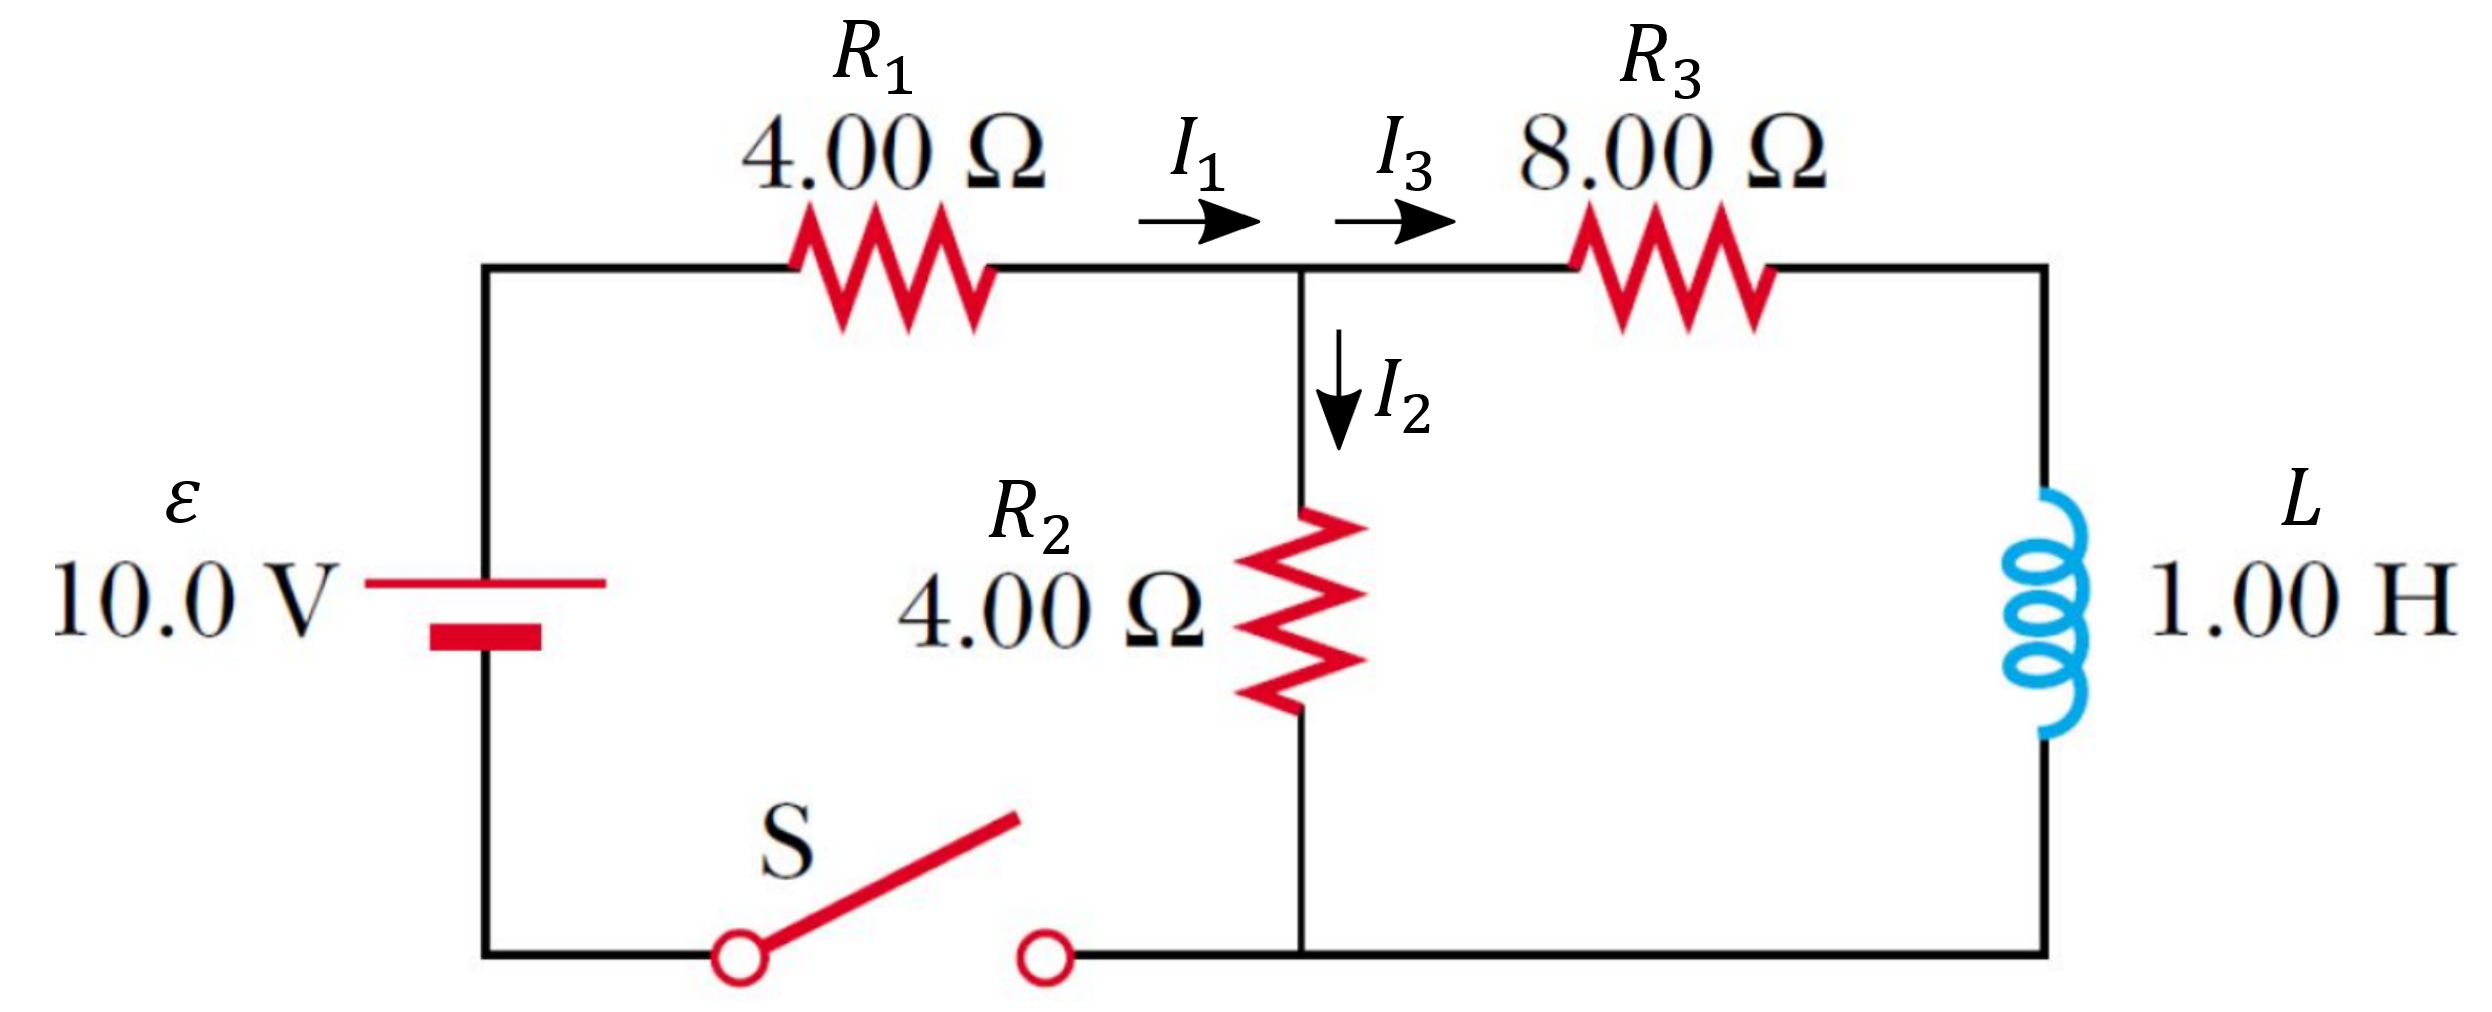
\includegraphics[width=8cm]{oz02/resources/oef-4-schets.png}
        % \end{figure}
    \item[Gevr. :]  $ \theta_e $; $ M_e $;
    \item[Opl. :] 
    (Oplossing van Serway 6E Chapter 29 Problem 22)

(a) Let $\theta$ represent the unknown angle; $L$, the total length of the wire; and $d$, the length of one side of the square coil. Then, using the definition of magnetic moment and the right-hand rule in Figure 29.15, we find
\\\\
$\mu=N A I$ :
$\boldsymbol{\mu}=\left(\frac{L}{4 d}\right) d^2 I$ at angle $\theta$ with the horizontal.
\\\\
At equilibrium,
$\sum \boldsymbol{\tau}=(\boldsymbol{\mu} \times \mathbf{B})-(\mathbf{r} \times m \mathbf{g})=0$
\\
$\left(\frac{I L B d}{4}\right) \sin \left(90.0^{\circ}-\theta\right)-\left(\frac{m g d}{2}\right) \sin \theta=0$
\\\\
and
$$
\begin{aligned}
& \left(\frac{m g d}{2}\right) \sin \theta=\left(\frac{I L B d}{4}\right) \cos \theta \\
& \theta=\tan ^{-1}\left(\frac{I L B}{2 m g}\right)=\tan ^{-1}\left(\frac{(3.40 \mathrm{~A})(4.00 \mathrm{~m})(0.0100 \mathrm{~T})}{2(0.100 \mathrm{~kg})\left(9.80 \mathrm{~m} / \mathrm{s}^2\right)}\right)=3.97^{\circ} .
\end{aligned}
$$
(b) $\quad \tau_m=\left(\frac{I L B d}{4}\right) \cos \theta=\frac{1}{4}(3.40 \mathrm{~A})(4.00 \mathrm{~m})(0.0100 \mathrm{~T})(0.100 \mathrm{~m}) \cos 3.97^{\circ}=3.39 \mathrm{mN} \cdot \mathrm{m}$
\end{description}

\vspace{1cm}

\newpage

\phantomsection
\label{OZ2:5}
\textbf{\underline{OZ 2 - Magnetische velden - Oefening 5:}}
\vspace{0.5cm}

Bereken het magnetisch dipoolmoment van een roterende geladen isolerende schijf
met straal $R$, waarbij de schijf rond zijn symmetrieas draait met een hoeksnelheid $\omega$
en de ladingsdichtheid varieert met de straal $r$ volgens $ \sigma = c \cdot r$, met $c$ een constante.

% \begin{description}[labelwidth=1.5cm, leftmargin=!]
%     \item[Geg. :]   
%     \item[Gevr. :]  
%     \item[Opl. :]  
% \end{description}


\begin{description}[labelwidth=1.5cm, leftmargin=!]
    \item[Geg. :]   $R,\omega, r, \sigma$
    \item[Gevr. :]  $\mu$
    \item[Opl. :]   
    
                    We stellen de formule van het infinitesimale oppervlakte op
                    \begin{align}
                         dA &= 2\pi rdr \nonumber \\ 
                        \intertext{waaruit we de formule voor de infinitesimale lading kunnen afleiden}
                         dq &= \sigma dA \nonumber \\ 
                            &= c2\pi r^2dr \\
                        \intertext{We weten de formule van de periode van de cirkelbeweging}
                          T &= \dfrac{2\pi}{\omega}  \\ 
                        \intertext{Uit (1) en (2) vinden we}
                         dI &= \dfrac{dq}{dt} \nonumber \\ 
                            &= \dfrac{dq}{T} \nonumber \\ 
                            &= \omega cr^2dr \nonumber \\
                        \intertext{waaruit we de infinitesimale magnetisch dipoolmoment kunnen halen}
                     d\mu &= dI(\pi r^2) \nonumber \\ 
                            % &= (\omega cr^2dr)(\pi r^2) \\ 
                            &= \pi\omega cr^4 dr \nonumber
                        \intertext{en dus het magnetisch dipoolmoment}
                        \mu &= \int_0^R d\mu \nonumber \\ 
                            &= \pi\omega \int_0^R r^4 dr \nonumber \\ 
                            &= \pi\omega c\tfrac{R^5}{5} \nonumber
                    \end{align}
\end{description} 

\vspace{1cm}



\newpage

\pagebreak

\fakesection{Oefenzitting 3}
% \subsection{De Lorentzkracht en de wet van Ampère}

\phantomsection
\label{OZ3:1}
\textbf{\underline{OZ 3 - De Lorentzkracht en de wet van Ampère - Oefening 1:}}
\vspace{0.5cm}

Bereken de kracht die inwerkt op een oneindig lange, rechte draad met stroom $I$ ten gevolge van:
\begin{enumerate}[(a)]
    \item de vierkante spoel
    \item de driehoekige spoel
\end{enumerate}

\begin{center}
    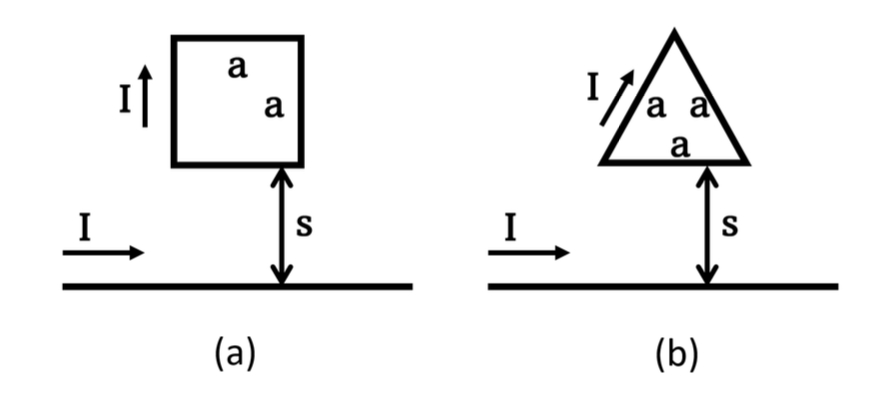
\includegraphics[scale = 0.5]{oz03/resources/Oz3Oef1.png}
\end{center}

% \begin{description}[labelwidth=1.5cm, leftmargin=!]
%     \item[Geg. :]   
%     \item[Gevr. :]  
%     \item[Opl. :]  
% \end{description}

\begin{enumerate}[(a)]
    \item 
        \begin{description}[labelwidth=1.5cm, leftmargin=!]
            \item[Geg. :]   $I$,$s$,$a$
            \item[Gevr. :]  de lorentzkracht $F_L$
            \item[Opl. :]   De evenwijdige zijden zullen een kracht uitoefenen op de draad. We vinden: 
                            \begin{align*}
                                F_L &= F_{\parallel, s+a} - F_{\parallel, s} \\ 
                                    % &= \dfrac{\mu_0I^2a}{2\pi}\left( \dfrac{1}{s+a} -\dfrac{1}{s} \right) \\
                                    &= \dfrac{\mu_0I^2}{2\pi}\dfrac{a^2}{s(s+a)} \\
                                \intertext{ Vectorieel wordt dit:}
                                \Vec{F}_L &= \dfrac{\mu_0I^2}{2\pi} \dfrac{a^2}{s(s+a)}(-\hat{j})
                            \end{align*}
        \end{description}
    \item 
        \begin{description}[labelwidth=1.5cm, leftmargin=!]
            \item[Geg. :]   $I$,$s$,$a$
            \item[Gevr. :]  de lorentzkracht $F_L$
            \item[Opl. :]   We berekenen eerst de infinitesimale kracht veroorzaakt door de schuine draden: 
                            \begin{equation*}
                                dF_{\text{schuin}} = \dfrac{\mu_0I^2\sin(60^\circ)}{2\pi}\dfrac{1}{r}dr
                            \end{equation*}
                            Hierover integreren we: 
                            \begin{align*}
                                F_{\text{schuin}} &= \int dF_{\text{schuin}} \\
                                                  &= \dfrac{\mu_0I^2}{2\pi\sin(60^\circ)} \int_s^{s+a\sin(60^\circ)} \tfrac{1}{r}dr \\
                                                  &= \dfrac{\mu_0I^2}{2\pi\sin(60^\circ)}\left(\ln(\tfrac{s+a\sin(60^\circ)}{s}) \right)
                            \end{align*}
                            Via superpositie vinden we: 
                            \begin{align*}
                                F_L &= 2F_{\text{schuin}} - F_{\parallel, s} \\
                                    &= \dfrac{\mu_0I^2}{2\pi}\left(\tfrac{1}{\sin(60^\circ)}\ln(\tfrac{s+a\sin(60^\circ)}{s}) - \dfrac{a}{s}\right)
                            \end{align*}
                            Vectorieel wordt dit:
                            \begin{equation*}
                                \Vec{F}_L = \dfrac{\mu_0I^2}{2\pi}\left( \tfrac{a}{s} - \tfrac{1}{\sin(60^\circ)}\left(\ln(\tfrac{s+a\sin(60^\circ)}{s}) \right) \right) (-\hat{j})
                            \end{equation*}
        \end{description}
        
\end{enumerate}

\vspace{1cm}

\newpage

\phantomsection
\label{OZ3:2}
\textbf{\underline{OZ 3 - De Lorentzkracht en de wet van Ampère - Oefening 2:}}
\vspace{0.5cm}

% \begin{description}[labelwidth=1.5cm, leftmargin=!]
%     \item[Geg. :]   
%     \item[Gevr. :]  
%     \item[Opl. :]  
% \end{description}

Een zeer groot geleidend vlak met dikte t draagt een uniforme stroomdichtheid $\Vec{j}$. Bepaal het magneetveld (grootte, richting en zin) op een afstand $y$ boven het vlak. (Neem aan dat het vlak oneindig groot is)

% \begin{center}
%     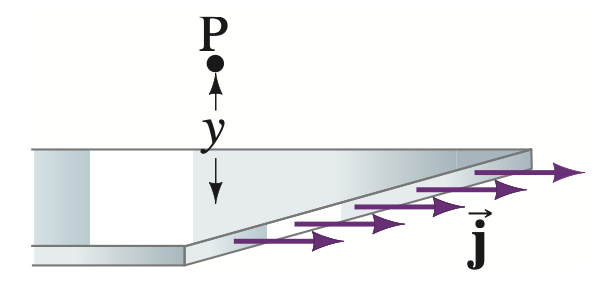
\includegraphics[scale = 0.4]{oz03/resources/Oz3Oef2.png}
% \end{center}

\begin{description}[labelwidth=1.5cm, leftmargin=!]
    \item[Geg. :] $t$, $\Vec{j}$, $y$
    \item[Gevr. :]  $\Vec{B}$ ?
    \item[Opl. :]
    \item[]
        \vspace{-0.7cm}
        \begin{minipage}{0.69\textwidth}
            The sheet may be treated as an infinite number of parallel wires. The magnetic field at a location y above the wire will be the sum of the magnetic fields produced by each of the wires. If we consider
            the magnetic field from two wires placed symmetrically on either side of where we are measuring the magnetic field, we see that the vertical magnetic field components cancel each other out. 
            Therefore, the field above the wire must be horizontal and to the left.  By symmetry, the field a location y below the wire must have the same magnitude, but point in the opposite direction. We calculate the magnetic field using Ampere’s law with a rectangular loop that extends a distance y above and below the current sheet, as shown in the figure.
            \begin{align*}
                \oint \Vec{B} \cdot d\Vec{\ell} = 2B_{\parallel}D &= \mu_0 I_{\text{in}} = \mu_0 (jtD) \\
                B_{\parallel} &= \tfrac{1}{2}\mu_0jt
            \end{align*}
        \end{minipage}
        \begin{minipage}{0.27\textwidth}
            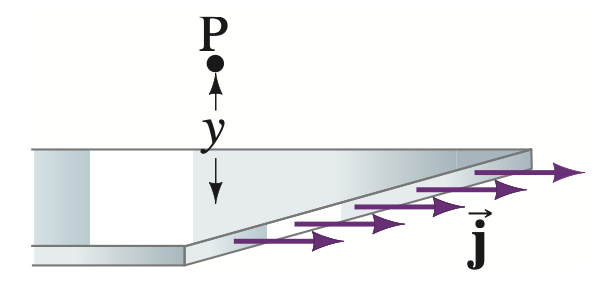
\includegraphics[scale = 0.4]{oz03/resources/Oz3Oef2.png} 
            \vspace{1cm}
            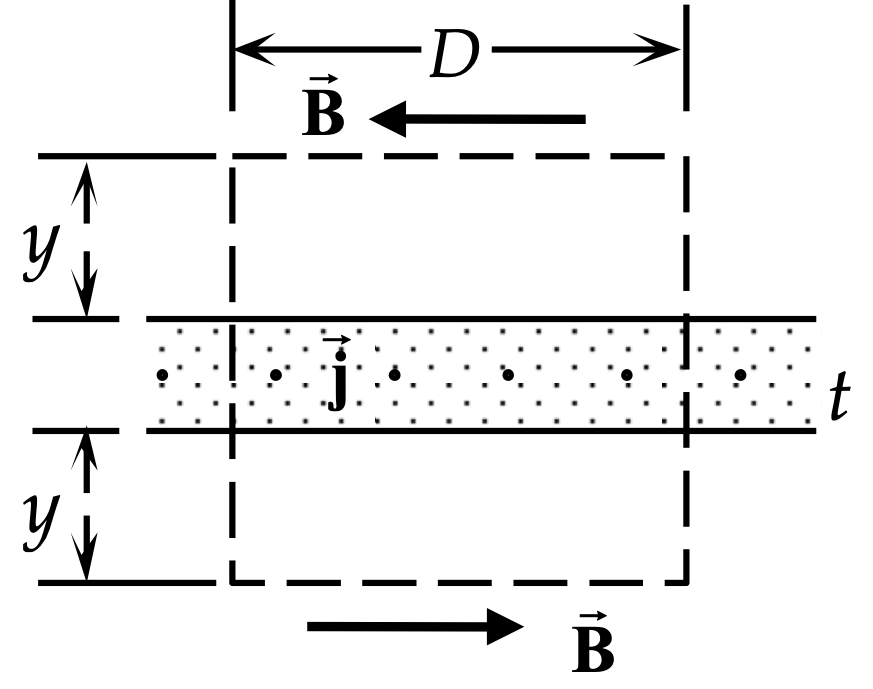
\includegraphics[scale = 0.275]{oz03/resources/Oz3Oef2Tekening.png}
        \end{minipage}

\end{description}

\vspace{1cm}

% \newpage

\phantomsection
\label{OZ3:3}
\textbf{\underline{OZ 3 - De Lorentzkracht en de wet van Ampère - Oefening 3:}}
\vspace{0.5cm}

% \begin{description}[labelwidth=1.5cm, leftmargin=!]
%     \item[Geg. :]   
%     \item[Gevr. :]  
%     \item[Opl. :]  
% \end{description}

Een zeer lange geleidende strip van breedte $d$ en verwaarloosbare dikte ligt in een horizontaal vlak en draagt een uniforme stroom $I$ door zijn cross sectie
\begin{enumerate}[(a)]
    \item 
        Toon aan dat voor punten op een afstand $y$ recht boven het centrum het magneetveld gegeven is door:
        \begin{equation*}
            B = \dfrac{\mu_0I}{\pi d}\tan^{-1}\left(\dfrac{d}{2y}\right)
        \end{equation*}
        Neem hierbij aan dat de strip oneindig lang is.
    \item 
        Weke waarde benadert $B$ voor $y >> d$? Houdt dit steek? Verklaar.
\end{enumerate}

\begin{enumerate}[(a)]
    \item 
        \begin{description}[labelwidth=1.5cm, leftmargin=!]
            \item[Geg. :]   $d$, $I$, $y$
            \item[Gevr. :]  $B$ ?
            \item[Opl. :]  
                        We kunnen een strip zien als een hoop infinitesimale draden over een breedte $d$. We zullen een
                        infinitesimale magnetisch veld bekijken dat veroorzaakt wordt door één van deze infinitesimale draden. Het $B_y$ veld zal nul worden, we bekijken dus $B_x$.
                        \begin{equation*}
                            dB_x 
                                = \frac{\mu_o}{2\pi}\frac{\sin(\theta)}{r} dI
                                = \frac{\mu_o I}{2\pi d}\frac{\sin(\theta)}{r} dx
                                = \frac{\mu_o I}{2\pi d}\frac{y}{x^2+y^2} dx
                        \end{equation*}
                        Het punt $y$ bevindt zich boven de oorsprong, we gebruiken symmetrie en integreren dus van $0\to\tfrac{d}{2}$: 
                        \begin{equation*}
                            B 
                                = \bigintsss_{\hspace{0.05cm} 0}^{\tfrac{d}{2}} \dfrac{\mu_oIy}{\pi d}\dfrac{dx}{x^2 + y^2} 
                                = \dfrac{\mu_oIy}{\pi d} \bigintsss_{\hspace{0.05cm} 0}^{\tfrac{d}{2}} \dfrac{dx}{x^2 + y^2}
                                = \dfrac{\mu_oI}{\pi d}\tan^{-1}(\tfrac{d}{2y})
                        \end{equation*}
        \end{description}
    \item 
        $\lim_{y\to\infty} \tan^{-1}(\tfrac{d}{2y}) = 0 \Rightarrow B = 0$
\end{enumerate}

\vspace{1cm}

\newpage

\phantomsection
\label{OZ3:4}
\textbf{\underline{OZ 3 - De Lorentzkracht en de wet van Ampère - Oefening 4:}}
\vspace{0.5cm}

% \begin{description}[labelwidth=1.5cm, leftmargin=!]
%     \item[Geg. :]   
%     \item[Gevr. :]  
%     \item[Opl. :]  
% \end{description}

\begin{minipage}{.76\textwidth}
    Hiernaast is een coaxiale kabel afgebeeld. Rond de binnenste geleider zit een isolerender laag, daarbuiten zit opnieuw een geleidende laag die afgeschermd wordt met een tweede laag isolatiemateriaal. De stroom door de binnenste draad is $1.00$ A \textbf{uit} het blad, de stroom door de buitenste geleider is $3.00$ A \textbf{in} het blad. Wat is de grootte, richting en zin van het magnetische veld in punten $a$ en $b$?

    \vspace{1cm}
\end{minipage}
\begin{minipage}{.2\textwidth}
    \vspace{-0.5cm}
    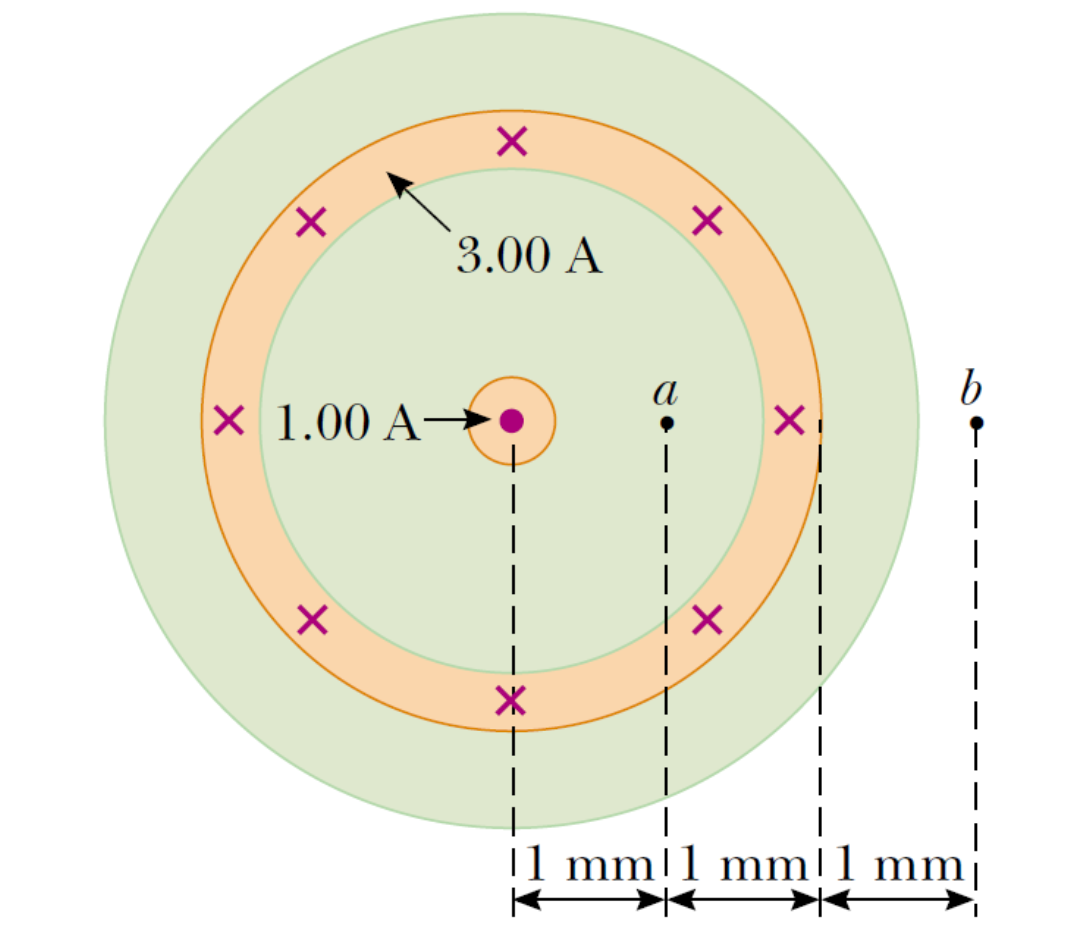
\includegraphics[scale = 0.225]{oz03/resources/Oz3Oef4.png}
\end{minipage}

\vspace{-0.9cm}

\begin{description}[labelwidth=1.5cm, leftmargin=!]
    \item[Geg. :]   $I_{\text{binnen}} = 1.00$ A, $I_{\text{buiten}} = 3.00$ A, $r_a = 1 \cdot 10^{-3}$ m, $r_b = 3r_a = 3 \cdot 10^{-3}$ m
    \item[Gevr. :]  $\Vec{B}_a$, $\Vec{B}_b$ ?
    \item[Opl. :]   
                    \begin{enumerate}[(a)]
                        \item
                            We passen de wet van ampère toe op het punt:
                            \begin{equation*}
                                B_a = \dfrac{\mu_0I_{\text{binnen}}}{2\pi r_a} = 2.00 \cdot 10^{-4} \text{ T}
                            \end{equation*}
                            Vectorieel wordt dit:
                            \begin{equation*}
                                \Vec{B}_a = 2.00 \cdot 10^{-4} \text{ T } \hat{j}
                            \end{equation*}
                            % sinds de ingesloten stroom uit het blad is.
                        \item 
                            We passen de wet van ampère toe op het punt:
                            \begin{equation*}
                                B_b = \dfrac{\mu_0}{2\pi r_a}(I_{\text{binnen}} + I_{\text{buiten}}) = -1.33 \cdot 10^{-4} \text{ T}
                            \end{equation*}
                            Vectorieel wordt dit:
                            \begin{equation*}
                                \Vec{B}_b = 1.33 \cdot 10^{-4} \text{ T }  (-\hat{j})
                            \end{equation*}
                            % sinds de ingesloten stroom in het blad is.
                    \end{enumerate}

                    
\end{description}

\vspace{1cm}


% \newpage

\phantomsection
\label{OZ3:5}
\textbf{\underline{OZ 3 - De Lorentzkracht en de wet van Ampère - Oefening 5:}}
\vspace{0.5cm}

Een solenoïde met diameter $10,0$ cm en lengte $75,0$ cm wordt gemaakt van een koperen
draad met een heel dunne laag isolatie. De diameter van de draad is $0,100$ cm.
De draad wordt in een enkele laag rond een kartonnen cilinder gewikkeld, waarbij
opeenvolgende wikkelingen elkaar raken. Welk vermogen moet geleverd worden aan
deze solenoïde om een veld van $8,00$ mT te creëeren in het centrum? De resistiviteit
van koper is $1.75 \cdot 10^{-8} \ \Omega$m bij $20^\circ$.

% \begin{description}[labelwidth=1.5cm, leftmargin=!]
%     \item[Geg. :]   
%     \item[Gevr. :]  
%     \item[Opl. :]  
% \end{description}

\begin{description}[labelwidth=1.5cm, leftmargin=!]
    \item[Geg. :]   $d_{\text{spoel}} = 10.0$ cm, $\ell_{\text{spoel}} = 75.0$ cm, $d_{\text{draad}} = 0.100$ cm, $\rho = 1.75 \cdot 10^{-8} \ \Omega$m, $B = 8.00$ mT
    % $T = 20^\circ$
    \item[Gevr. :]  $P$ ?
    \item[Opl. :]   
    
                    We passen de wet van ampère toe 
                    \begin{equation*}
                        \oint \Vec{B} \cdot d\Vec{\ell} = B\ell_{\text{spoel}} = \mu_0NI_{\text{in}}
                    \end{equation*}
                    Er is gegeven dat opeenvolgende wikkelingen elkaar raken, hieruit volgt dat 
                    \begin{equation*}
                        B = \mu_0\dfrac{N}{\ell_{\text{spoel}}}I_{\text{in}} = \mu_0d_{\text{draad}}I_{\text{in}} 
                    \end{equation*}
                    sinds $N = \tfrac{\ell_{\text{spoel}}}{d_{\text{draad}}}$. We vervangen $I_{\text{in}}$ met $\sqrt{\tfrac{P}{R}}$:
                    \begin{equation*}
                        B = \mu_0\sqrt{\dfrac{P}{R}} = \mu_0\sqrt{\dfrac{P}{4\rho\dfrac{\ell_{\text{draad}}}{\pi d_{\text{draad}}^2}}}
                    \end{equation*}
                    De lengte van de draad kunnen we berekenen met
                    \begin{equation*}
                        \ell_{\text{draad}} = \pi d_{\text{spoel}} N 
                    \end{equation*}
                    Hieruit kunnen we P berekenen: 
                    \begin{equation*}
                        P = \left(\dfrac{B}{\mu_0}\right)^2\left(4\rho N \dfrac{d_{\text{spoel}}}{
                        d_{\text{draad}}^2}\right) \approx 213 W
                    \end{equation*}           
\end{description}

\vspace{1cm}

\newpage

\pagebreak

\fakesection{Oefenzitting 4}

\phantomsection
\label{OZ4:1}
\textbf{\underline{OZ 4 - De wet van Ampère en de wet van Biot-Savart - Oefening 1:}}
\vspace{0.5cm}

Een geleider bestaat uit een cirkelvormige lus met straal $R$ en twee lange rechte stukken. De draad ligt in het vlak van het blad en er loopt een stroom $I$ doorheen. Bepaal de grootte en de richting van het magnetische veld dat geproduceerd wordt in het centrum van de lus.

\begin{center}
    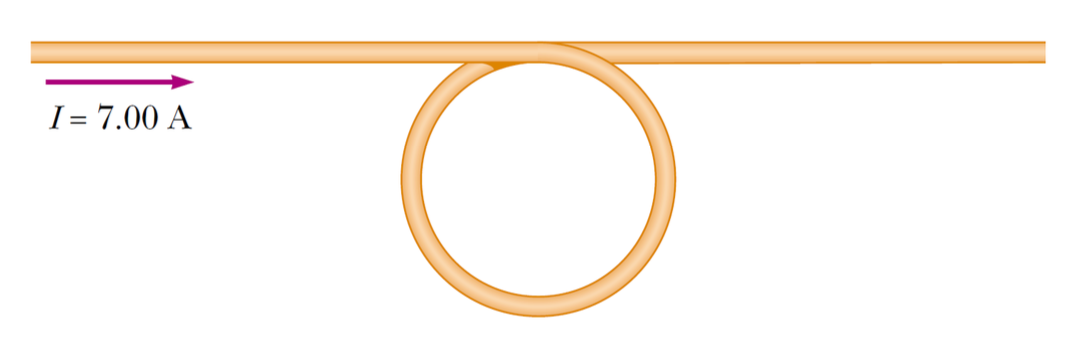
\includegraphics[scale = 0.5]{oz04/resources/Oz4Oef1.png}
\end{center}

\begin{description}[labelwidth=1.5cm, leftmargin=!]
    \item[Geg. :]   $I = 7.00$A, $R$
    \item[Gevr. :]  $\Vec{B}$ ?
    \item[Opl. :]  
    Stel nu dat $d\ell$ een infinitesimaal deeltje cirkelboog, dan is het infinitesimaal magnetisch veld door de lus
    \begin{align*}
        dB_L
            &= \frac{\mu_0I}{4\pi}\frac{d\ell}{R^2} \\
            &= \frac{\mu_0I}{4\pi}\frac{\sin(\gamma)}{R}d\theta \\
            &\overset{\perp}{=} \frac{\mu_0I}{4\pi}\frac{d\theta}{R} 
    \end{align*}
    waarbij $\gamma$ de hoek is tussen $\Vec{r}$ en $d\Vec{\ell}$ hierover integreren om het totale magnetische veld te bekomen
    \begin{align*}
        B_L
            &= \int_{0}^{2\pi} \frac{\mu_0I}{4\pi}\frac{d\theta}{R}  \\
            &= \frac{\mu_0I}{4\pi R} \int_{0}^{2\pi}d\theta \\
            &=  \frac{\mu_0I}{2R}
    \end{align*}
    Het bovenste punt zou twee keer moeten meegtelt worden, omdat er een overlap is (de andere overlap is niet loodrecht boven het punt en zal dus volgens de wet van ampere ons magnetisch veld niet beinvloeden). Dus tellen we er nog een factor
    \begin{equation*}
        B_P = \frac{\mu_0}{2\pi}\frac{I}{R}
    \end{equation*}
    bij en vervolgens krijgen we
    \begin{equation*}
        \Vec{B} = \Vec{B}_L + \Vec{B}_P = \frac{\mu_0I}{2R}\left(\frac{1}{\pi} + 1\right)(-\hat{k})
    \end{equation*}
    waarbij de rechterhandregel geeft dat het in het blad is.
\end{description}

\vspace{1cm}

\newpage

\phantomsection
\label{OZ4:2}
\textbf{\underline{OZ 4 - De wet van Ampère en de wet van Biot-Savart - Oefening 2:}}
\vspace{0.5cm}

\begin{minipage}{0.7\textwidth}
    Een circuit bestaat uit twee bogen met straal $R$ en twee rechte stukken op een afstand $2a$ van elkaar. Door het circuit loopt een stroom $I$. Bereken het magneetveld $\vec{B}$ in het punt $P = 0$, gelegen in het vlak van het circuit
    \vspace{1.5cm}
\end{minipage}
\begin{minipage}{0.26\textwidth}
    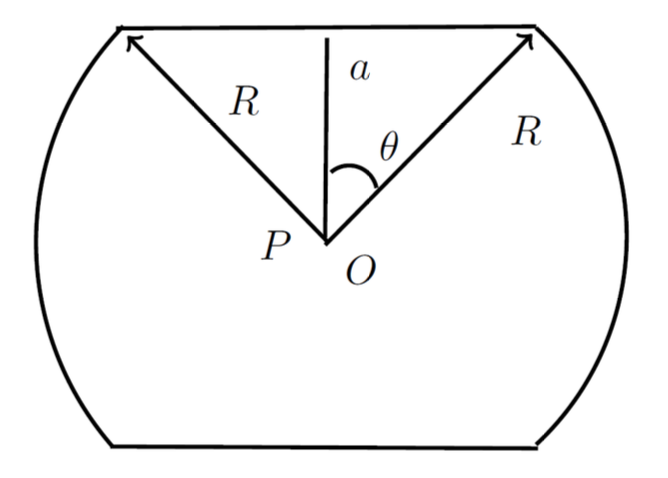
\includegraphics[scale = 0.35]{oz04/resources/Oz4Oef2.png}
\end{minipage}

% \begin{center}
%     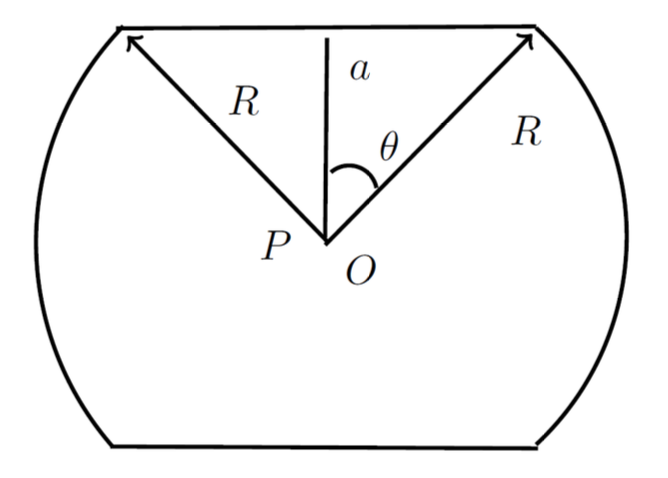
\includegraphics[scale = 0.4]{oz04/resources/Oz4Oef2.png}
% \end{center}
\vspace{-1.5cm}

\begin{description}[labelwidth=1.5cm, leftmargin=!]
    \item[Geg. :]   $R$, $a$, $I$
    \item[Gevr. :]  $\Vec{A}$ ?
    \item[Opl. :]  
    We zullen de vectoriële aanbrenging van de rechte stukken en bogen apart berekenen:
    \begin{itemize}
        \item 
            We integreren over alle infinitesimale magnetische velden geproduceerd door een rechte stuk 
            \begin{align*}
                \vec{B}_{|} 
                    &= \int d\Vec{B}_{|} \\
                    &= \frac{\mu_0I}{4\pi}\int\frac{d\ell}{r^2} \sin(\phi) \ (-\hat{k}) \\
                    &= \frac{\mu_0I}{4\pi}\frac{1}{a} \int \sin(\phi) d\phi  \ (-\hat{k}) \\
                    &= \frac{\mu_0I}{2\pi}\frac{1}{a} \int_{\phi}^{\frac{\pi}{2}} \sin(\phi) d\phi  \ (-\hat{k}) \\
                    &= \frac{\mu_0I}{2\pi}\frac{1}{a} \cos(\phi) \ (-\hat{k}) \\
                    &= \frac{\mu_0I}{2\pi}\frac{1}{a} \frac{\sqrt{R^2-a^2}}{R} \ (-\hat{k}) \\
            \end{align*}
            waarbij we gebruikt hebben dat
            \begin{equation*}
                \frac{1}{r^2} = \frac{\sin^2(\phi)}{a^2}  \quad \text{en} \quad d\ell = d\left(\frac{a}{\tan(\phi)}\right) = \frac{a}{\sin^2(\phi)}d\phi.       
            \end{equation*}
        \item 
            We berekenen het infinitesimale veld geproduceerd door de bogen, we beginnen eerst voor een boog en maken gebruik van $\phi$ van bij de rechte stukken
            \begin{align*}
                d\Vec{B}_{\sim} 
                    &= \frac{\mu_0I}{4\pi}\frac{d\ell \sin(\gamma)}{R^2} \ (-\hat{k}) \\
                    &\overset{\perp}{=} \frac{\mu_0I}{4\pi}\frac{d\ell}{R^2} \ (-\hat{k}) \\
                    &= \frac{\mu_0I}{4\pi}\frac{d\phi}{R} \ (-\hat{k}) 
            \end{align*}
            waarbij $\gamma$ de (loodrechte) hoek is tussen $d\ell$ en $\hat{r}$. We integreren nu over de volledige boog:
            \begin{align*}
                \Vec{B}_{\sim} 
                    &= \int d\Vec{B}_{\sim} \\
                    &= \frac{\mu_0I}{4\pi}\frac{1}{R} \int_{-\phi}^{\phi} d\phi \ (-\hat{k}) \\
                    &= \frac{\mu_0I}{2\pi}\frac{1}{R} \phi \ (-\hat{k}) \\
                    &= \frac{\mu_0I}{\pi R}\left(\frac{\pi}{2}-\sin^{-1}\left(\frac{\sqrt{R^2-a^2}}{R}\right)\right) \ (-\hat{k}) 
            \end{align*}
    \end{itemize}
    De rechten en kromme stukken zullen elkaar versterken, dus vinden we voor de totale vectoriële som:
    \begin{equation*}
        \Vec{B} = 2(\vec{B}_{|} + \Vec{B}_{\sim}) = \frac{\mu_0I}{\pi R}\left(\frac{1}{a}\sqrt{R^2-a^2} + \frac{\pi}{2} -\sin^{-1}\left(\frac{\sqrt{R^2-a^2}}{R}\right) \right)
    \end{equation*}
    
\end{description}

\vspace{1cm}

\newpage

\phantomsection
\label{OZ4:3}
\textbf{\underline{OZ 4 - De wet van Ampère en de wet van Biot-Savart - Oefening 3:}}
\vspace{0.5cm}

\begin{minipage}{0.7\textwidth}
    \vspace{-2cm}
    Een niet-geleidende schijf van straal $R$ draagt een uniform verdeelde lading $Q$. De schijf wordt rondgedraaid met een hoeksnelheid $\omega$ rond een as loodrecht op het vlak
    van de schijf en door het centrum van de schijf.
\end{minipage}
\begin{minipage}{0.26\textwidth}
    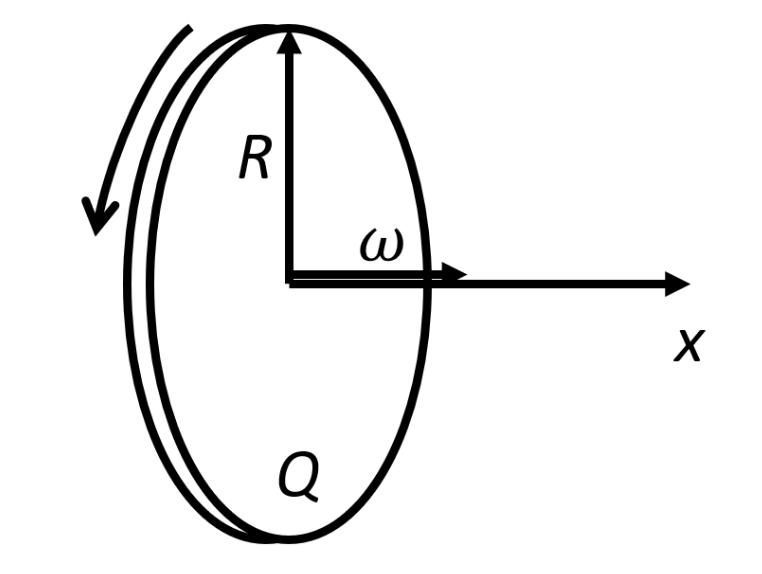
\includegraphics[scale = 0.3]{oz04/resources/Oz4Oef3.png}
\end{minipage}

\vspace{-2cm}

% \begin{description}[labelwidth=1.5cm, leftmargin=!]
%     \item[Geg. :]  
%     \item[Gevr. :] 
%     \item[Opl. :]  
% \end{description}

\begin{enumerate}[(a)]
    \item Bepaal het magnetische dipoolmoment van de schijf.
    \item Bepaal het magnetische veld op de rotatie-as op een afstand $x$ 
          \\ van het centrum van de schijf.
    \item Als $x >> R$ reduceert de uitkomst van (b) dan naar de formule
          \\ voor een magnetische dipool?
\end{enumerate}

\begin{enumerate}[(a)]
    \item 
        \begin{description}[labelwidth=1.5cm, leftmargin=!]
            \item[Geg. :]  $R$, $Q$, $\omega$
            \item[Gevr. :] $\Vec{\mu}$ ?
            \item[Opl. :]  
                         We stellen de formule van het infinitesimale oppervlakte op
                         \begin{align}
                             dA &= 2\pi rdr \nonumber \\ 
                            \intertext{waaruit we de formule voor de infinitesimale lading kunnen afleiden}
                             dq &= \dfrac{Q}{A} dA \nonumber \\ 
                                &= \dfrac{Q}{R^2}2rdr \\
                            \intertext{We weten de formule van de periode van de cirkelbeweging}
                            T &= \dfrac{2\pi}{\omega}  \\ 
                            \intertext{Uit (1) en (2) vinden we}
                             dI &= \dfrac{dq}{dt} \nonumber \\ 
                                &= \dfrac{dq}{T} \nonumber \\ 
                                &= \dfrac{Q\omega}{R^2\pi}rdr \nonumber \\
                                % &= \omega r^2dr \nonumber \\
                            \intertext{waaruit we de infinitesimale magnetisch dipoolmoment kunnen halen}
                           d\mu &= dI(\pi r^2) \nonumber \\ 
                                % &= (\omega cr^2dr)(\pi r^2) \\ 
                                &= \dfrac{Q\omega}{R^2}r^3 dr \nonumber
                            \intertext{en dus het magnetisch dipoolmoment}
                            \mu &= \int_0^R d\mu \nonumber \\ 
                                &= \dfrac{Q\omega}{R^2} \int_0^R r^3 dr \nonumber \\ 
                                &= \dfrac{Q \omega R^2}{4} \nonumber \\
                            \intertext{Vectorieel wordt dit:}
                            \Vec{\mu} &= \dfrac{Q \omega R^2}{4} \hat{i} \nonumber
                         \end{align}
        \end{description}
        \newpage
        
    \item 
        \begin{description}[labelwidth=1.5cm, leftmargin=!]
            \item[Geg. :]  $R$, $Q$, $\omega$
            \item[Gevr. :] $B_x$ ?
            \item[Opl. :]  
                        We berekenen eerst het magnetisch veld in het centrum van een cirkel met straal $r$
                        \begin{align*}
                            B_{\text{cirkel},x} 
                                &= \frac{\mu_0I}{4\pi} \int \frac{d\ell}{r^2 + x^2} \sin(\phi) \\
                                &= \frac{\mu_0I}{4\pi} \int \frac{r}{r^2 + x^2} \sin(\phi) d\theta \\
                                &= \frac{\mu_0I}{4\pi}  \int \frac{r}{r^2 + x^2} \frac{r}{\sqrt{r^2+x^2}} d\theta \\
                                &= \frac{\mu_0 Q\omega r}{4\pi^2 R^2} \frac{r}{r^2 + x^2} \frac{r}{\sqrt{r^2+x^2}} \int_0^{2\pi} d\theta \\
                                &= \frac{\mu_0 Q\omega r^3}{2\pi R^2(r^2 + r^2)^{\tfrac{3}{2}}} \\
                                \intertext{
                                    waarbij $I = \frac{Q\omega}{R^2\pi}r$, wat we berekent hadden in (a).  Een schijf bestaat uit infinitesimale cirkels en dus integreren we over bovenstaande formule om het magnetisch veld door de schijf te verkrijgen
                                }
                                B_{\text{schijf},x} 
                                &= \int dB_{\text{cirkel},x} \\
                                % &= \int \frac{\mu_0dI}{2\pi} \frac{r^2}{(r^2 + x^2)^{\tfrac{3}{2}}} \\
                                &= \int \frac{\mu_0 Q\omega r^3}{2\pi R^2(r^2 + r^2)^{\tfrac{3}{2}}}  dr \\
                                % &= \int \frac{\mu_0}{2\pi} \frac{Q\omega r}{\pi R^2} \frac{r^2}{(r^2 + x^2)^{\tfrac{3}{2}}} dr \\
                                &= \frac{\mu_0Q\omega}{2\pi R^2} \int_0^R \frac{r^3}{(r^2 + x^2)^{\tfrac{3}{2}}} \\
                                &= \frac{\mu_0Q\omega}{2\pi R^2}\left(\sqrt{x^2+R^2} + \frac{x^2}{\sqrt{x^2+R^2}} - 2x\right) 
                        \end{align*}
        \end{description}
        
    \item 
        \begin{description}[labelwidth=1.5cm, leftmargin=!]
            \item[Geg. :]  $x >> R$, $ B_{\text{dipool}} \approx \frac{\mu_0}{2\pi} \frac{\mu}{x^3}$
            \item[Gevr. :] $ B_{\text{schijf},x} \approx B_{\text{dipool}}$ ?
            \item[Opl. :]  
            We beginnen door $B_{\text{schijf},x}$ te herschrijven
            \begin{align*}
                B_{\text{schijf},x}
                    &= \frac{\mu_0Q\omega}{2\pi R^2}\left(\sqrt{x^2+R^2} + \frac{x^2}{\sqrt{x^2+R^2}} - 2x\right) \\
                    &= \frac{\mu_0Q\omega x}{2\pi R^2}\left(\sqrt{1+\frac{R^2}{x^2}} + \frac{1}{\sqrt{1+\frac{R^2}{x^2}}} - 2\right) 
            \end{align*}
            We nemen de derde-orde taylorreeks van $\sqrt{1+y^2}$ en $(\sqrt{1+y^2})^{-1}$ 
            \begin{align*}
                \sqrt{1+y^2} 
                    &= 1 + \frac{1}{2}y - \frac{1}{8}y^2 \\
                \frac{1}{\sqrt{1+y^2}} 
                    &=  1 - \frac{1}{2}y + \frac{3}{8}y^2 \\
            \end{align*}
            waaruit volgt
            \begin{equation*}
                 B_{\text{schijf},x} = \frac{\mu_0Q\omega R^2}{8\pi x^3} = \frac{\mu_0}{2\pi} \frac{\mu}{x^3} \approx B_{\text{dipool}}                  
            \end{equation*}
        \end{description}
\end{enumerate}


\vspace{1cm}

\newpage

\phantomsection
\label{OZ4:4}
\textbf{\underline{OZ 4 - De wet van Ampère en de wet van Biot-Savart - Oefening 4:}}
\vspace{0.5cm}

Bepaal de grootte, richting en zin van het magnetische veld dat geproduceerd wordt
in het punt $P$ door de stroomvoerende lus.

\begin{center}
    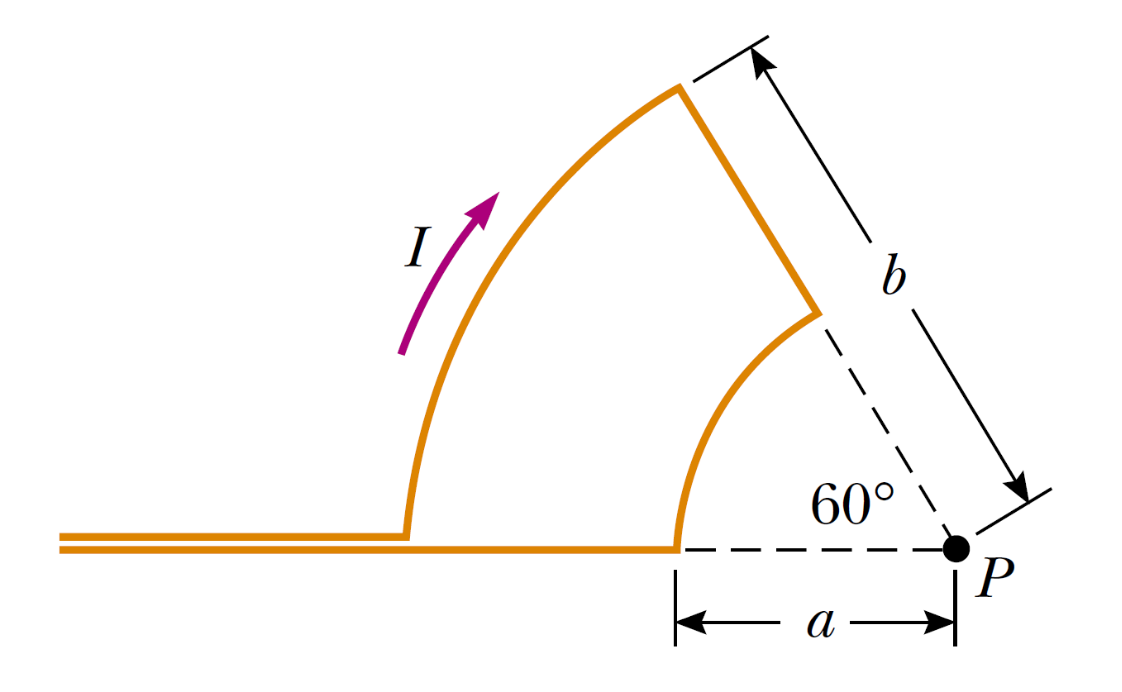
\includegraphics[scale = 0.3]{oz04/resources/Oz4Oef4.png}
\end{center}

% \begin{description}[labelwidth=1.5cm, leftmargin=!]
%     \item[Geg. :]   
%     \item[Gevr. :]  
%     \item[Opl. :]  
% \end{description}

\begin{description}[labelwidth=1.5cm, leftmargin=!]
    \item[Geg. :]  $a$, $b$, $\theta$
    \item[Gevr. :] $\Vec{B}$ ?
    \item[Opl. :]  
    Het magnetisch veld zal bepaald worden door de twee booglengtes. 
    \begin{enumerate}[(a)]
        \item 
        Het magnetische veld door de dichtste booglengte is
        \begin{equation*}
            \Vec{B}_a = \frac{\mu_0I}{4a\pi}\int_0^{\theta}ds \ (\hat{k}) = \frac{\mu_0I\theta}{4a\pi} \ (\hat{k})
        \end{equation*}
        \item 
        Het magnetische veld door de verste booglengte is
        \begin{equation*}
            \Vec{B}_b = \frac{\mu_0I}{4b\pi}\int_0^{\theta}ds \ (-\hat{k}) = \frac{\mu_0I\theta}{4b\pi} \ (-\hat{k})
        \end{equation*}
    \end{enumerate}
    De vectorsom hiervan is dan
    \begin{equation*}
        \Vec{B} = \Vec{B}_a + \Vec{B}_b = \frac{\mu_0I\theta}{4\pi}\left(\frac{1}{a}-\frac{1}{b}\right) \ (\hat{k})
    \end{equation*}
    waarbij $\theta = \dfrac{\pi}{3}$.
\end{description}

\vspace{1cm}

\newpage

\phantomsection
\label{OZ4:5}
\textbf{\underline{OZ 4 - De wet van Ampère en de wet van Biot-Savart - Oefening 5:}}
\vspace{0.5cm}

% \begin{minipage}{0.64\textwidth}
%     Een lange cilindrische geleider met straal $a$ heeft twee cilindrische gaten van diameter $a$ doorheen zijn hele lengte (zie doorsnede in Figuur 5). Een stroom $I$ vloeit door de geleider en is uit het blad gericht. De stroomdichtheid is uniform doorheen de doorsnede van de draad. Wat is het magnetisch veld in termen van $\mu_0$, $I$, $r$ en $a$ in punt $P_1$? Dezelfde vraag voor punt $P_2$.
%     \vspace{1cm}
% \end{minipage}
% \begin{minipage}{0.32\textwidth}
%     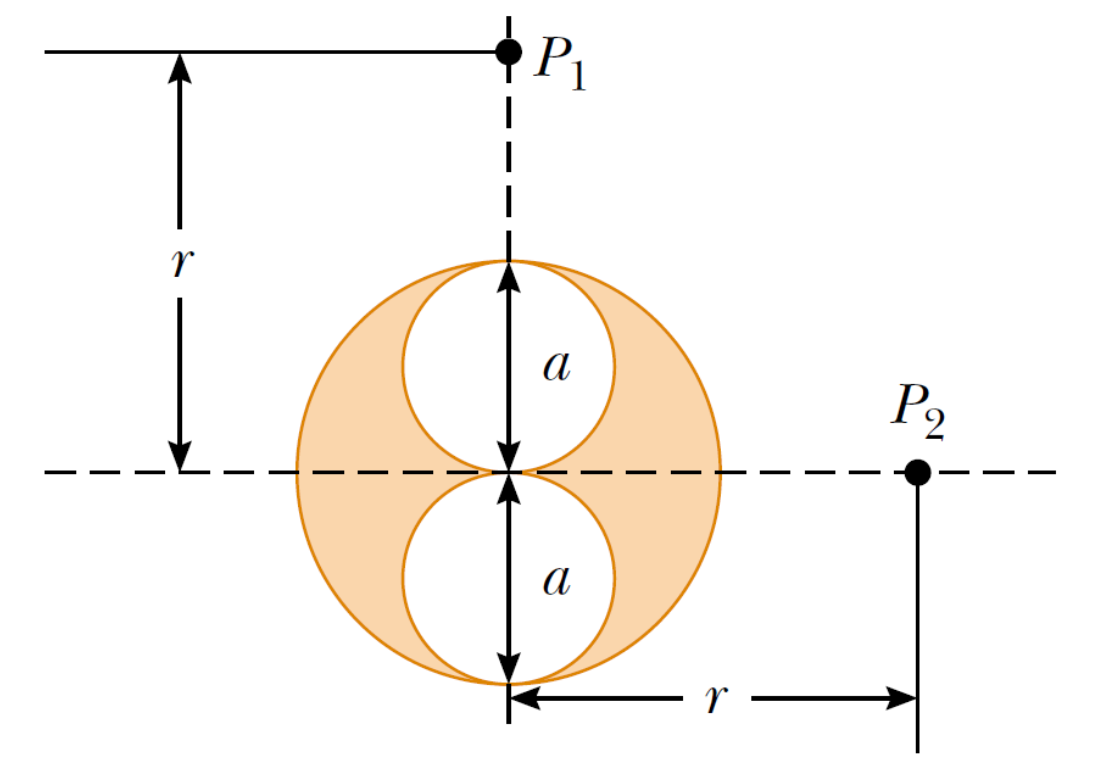
\includegraphics[scale = 0.25]{oz04/resources/Oz4Oef5.png}
% \end{minipage}

% \vspace{-1cm}

Een lange cilindrische geleider met straal $a$ heeft twee cilindrische gaten van diameter $a$ doorheen zijn hele lengte (zie doorsnede in Figuur 5). Een stroom $I$ vloeit door de geleider en is uit het blad gericht. De stroomdichtheid is uniform doorheen de doorsnede van de draad. Wat is het magnetisch veld in termen van $\mu_0$, $I$, $r$ en $a$ in punt $P_1$? Dezelfde vraag voor punt $P_2$.
    
\begin{center}
    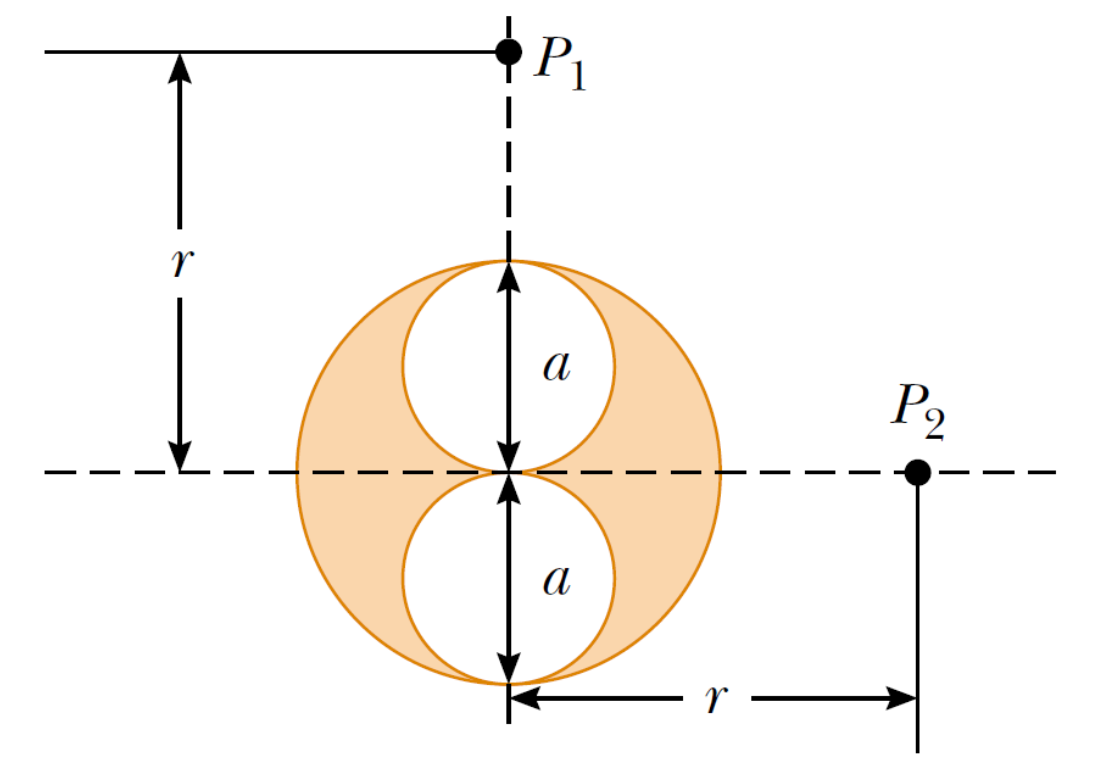
\includegraphics[scale = 0.3]{oz04/resources/Oz4Oef5.png}
\end{center}

% \begin{description}[labelwidth=1.5cm, leftmargin=!]
%     \item[Geg. :]   
%     \item[Gevr. :]  
%     \item[Opl. :]  
% \end{description}

% De oppervlakte is gelijk aan
% \begin{equation*}
%     A = \pi a^2 - 2\pi \left(\frac{a}{2}\right)^2 = \pi \frac{a^2}{2}
% \end{equation*}

\begin{description}[labelwidth=1.5cm, leftmargin=!]
    \item[Opl. :]  
    
        Neem $B_1$ het magnetisch veld door het gekleurde deel, $B_2$ het magnetisch veld door de bovenste caviteit en $B_3$ het magnetisch veld door de onderste caviteit.
        De oppervlakte $A$ waardoor stroom vloeit is
        \begin{equation*}
            A = \pi\left(a^2 - \frac{a^2}{2}\right) = \pi\frac{a^2}{2}
        \end{equation*}
        waaruit volgt dat de stroom dichtheid $J$ het volgende is
        \begin{equation*}
            J = \frac{2I}{\pi a^2}
        \end{equation*}
        m.a.w. er vloeit een stroom $2I$ door de geleider (en dus een stroom $-I$ door de caviteiten). \\
        
        \begin{enumerate}[$P_1$:]    
            \item 
                \begin{description}[labelwidth=1.5cm, leftmargin=!]
                    \item[Geg. :]  $\mu_0$, $I$, $r$, $a$
                    \item[Gevr. :] $B$ in $P_1$ ?
                    \item[Opl. :]  
                    We vinden de volgende magnetische velden
                    \begin{align*}
                        \vec{B}_1 
                            &= \frac{\mu_0Ja^2}{r} \ (\hat{i}) \\
                        \vec{B}_2
                            &= \frac{\mu_0J(\frac{a}{2})^2}{2\left(r - \frac{a}{2}\right)} \ (-\hat{i}) \\
                        \vec{B}_3 
                            &= \frac{\mu_0J(\frac{a}{2})^2}{2\left(r + \frac{a}{2}\right)} \ (-\hat{i})
                    \end{align*}
                    het totale veld in $P_1$ is
                    \begin{align*}
                        \vec{B} 
                            &= \sum_{i=1}^3 B_i \ (\hat{i}) \\
                            &= \frac{\mu_0Ja^2}{2} \left[\frac{1}{r} - \frac{1}{4\left(r - \left(\frac{a}{2}\right)\right)} - \frac{1}{4\left(r + \left(\frac{a}{2}\right)\right)} \right] \\
                            &= \frac{\mu_0I}{\pi r}\left(\frac{2r^2-a^2}{4r^2-a^2}\right) \ (-\hat{i}).
                    \end{align*}
                    % Vectorieel:
                    % \begin{equation*}
                    %     \Vec{B} = \frac{\mu_0I}{\pi r}\left(\frac{2r^2-a^2}{4r^2-a^2}\right) \ (-\hat{i})
                    % \end{equation*}
                \end{description}    
            \item 
                \begin{description}[labelwidth=1.5cm, leftmargin=!] 
                    \item[Geg. :]  $\mu_0$, $I$, $r$, $a$
                    \item[Gevr. :] $B$ in $P_2$ ?
                    \item[Opl. :]  
                     We vinden de volgende magnetische velden
                    \begin{align*}
                        \vec{B}_1 
                            &= \frac{\mu_0Ja^2}{2r} \ (\hat{j}) \\
                        \vec{B}_{2,3} 
                            &=  \frac{\mu_0J(\frac{a}{2})^2}{2 \sqrt{r^2 + \left(\frac{a}{2}\right)^2}} \ (-\hat{j})
                    \end{align*}
                    waarbij $B_{2,3} = B_2 = B_3$. De horizontale componenten van $B_2$ en $B_3$ doen elkaar te niet, het totale veld in $P_2$ is
                    \begin{align*}
                        \vec{B} 
                            &= \sum_{i=1}^3 B_i \ (\hat{j}) \\
                            &= \frac{\mu_0Ja^2}{2r} - \left(\frac{\mu_0J(\frac{a}{2})^2}{\sqrt{r^2 + \left(\frac{a}{2}\right)^2}}\frac{r}{\sqrt{r^2 + \left(\frac{a}{2}\right)^2}}\right) \ (\hat{j}) \\
                            &= \frac{\mu_0Ja^2}{2r}\left[1 - \frac{r^2}{2\left(r^2 + \left(\frac{a}{2}\right)^2\right)}\right] \ (\hat{j}) \\
                            &=\frac{\mu_0I}{\pi r}\left(\frac{2r^2+a^2}{4r^2+a^2}\right) \ (\hat{j}).
                    \end{align*}
                    % \begin{align*}
                    %     \vec{B} 
                    %         &= B_1 - 2B_{2,3}\cos(\theta) \ (\hat{j}) \\
                    %         &= \frac{\mu_0I}{\pi r} - \frac{\mu_0I}{\pi \sqrt{r^2 + \left(\frac{a}{2}\right)^2}}\cos(\theta) \\ 
                    %         &= \frac{\mu_0I}{\pi r} - \frac{\mu_0I}{\pi \sqrt{r^2 + \left(\frac{a}{2}\right)^2}} \frac{r}{\sqrt{r^2 + \left(\frac{a}{2}\right)^2}} \\ 
                    %         &= \frac{\mu_0I}{\pi r}\left(1 - \frac{r^2}{r^2 + \left(\frac{a}{2}\right)^2} \right) \\
                    %         &=\frac{\mu_0I}{\pi r}\left(\frac{2r^2+a^2}{4r^2+a^2}\right)\ (\hat{j})
                    % \end{align*}    
                \end{description}
        \end{enumerate}

\end{description}
\vspace{1cm}

\newpage

\pagebreak

\fakesection{Oefenzitting 5}

\phantomsection
\label{OZ5:1}
\textbf{\underline{OZ 5 - Magnetische inductie en de wet van Faraday - Oefening 1:}}
\vspace{0.5cm}

\begin{minipage}{0.76\textwidth}
    Een segment van een draad met lengte $d$ draagt een stroom $I$, zoals aangegeven in de figuur hiernaast.

    \begin{enumerate}[(a)]
        \item 
            Toon aan dat voor punten op de positieve $x$-as, zoals het punt $Q$, het magnetisch veld $\Vec{B}$ nul is.
        \item 
            Bepaal de uitdrukking van het magnetisch veld $\Vec{B}$ voor punten op de positieve $y$-as, zoals het punt $P$.
    \end{enumerate}
\end{minipage}
\begin{minipage}{0.2\textwidth}
    \begin{center}
        \includegraphics[scale = 0.35]{oz05/resources/Oz5Oef1.png}
    \end{center}
\end{minipage}

\begin{enumerate}[(a)]
    \item 
        \begin{description}[labelwidth=1.5cm, leftmargin=!]
            \item[Geg. :]  $Q$, $d$, $I$
            \item[Gevr. :] $\Vec{B}$
            \item[Opl. :]  
                We gebruiken de wet van Biot-Savart
                \begin{equation*}
                    \Vec{B} = \frac{\mu_0}{4\pi} \int \frac{Id\Vec{\ell} \times \hat{r}}{r^2} = \Vec{0}
                \end{equation*}
                waarbij $r$ en elke infinitesmiale $d\ell$ parallel zijn.
        \end{description}
    \item 
        \begin{description}[labelwidth=1.5cm, leftmargin=!]
            \item[Geg. :]  $P$, $d$, $I$
            \item[Gevr. :] $\Vec{B}$
            \item[Opl. :]   
                We gebruiken de wet van Biot-Savart
                \begin{align*}
                    \Vec{B} 
                        &= \frac{\mu_0}{4\pi} \int \frac{Id\Vec{\ell} \times \hat{r}}{r^2} \\
                        &= \frac{\mu_0I}{4\pi} \int \frac{d\Vec{\ell} \times \Vec{r}}{r^3} \\
                        &= \frac{\mu_0I}{4\pi} \int \frac{dx\hat{i}\times(-x\hat{i} + y\hat{j})}{(x^2 + y^2)^{\frac{3}{2}}} \\
                        &= \frac{\mu_0Iy}{4\pi} \int_0^d \frac{dx}{(x^2 + y^2)^{\frac{3}{2}}} \ (\hat{k}) \\
                        &= \frac{\mu_0Iy}{4\pi} \left[ \frac{x}{y^2(x^2 + y^2)^{\frac{1}{2}}} \right]_0^d \ (\hat{k}) \\
                        &= \frac{\mu_0I}{4\pi y} \frac{d}{(d^2 + y^2)^{\frac{1}{2}}} \ (\hat{k}) \\
                \end{align*}
        \end{description}
\end{enumerate}
    
\vspace{1cm}

\newpage

\phantomsection
\label{OZ5:2}
\textbf{\underline{OZ 5 - Magnetische inductie en de wet van Faraday - Oefening 2:}}
\vspace{0.5cm}


\begin{minipage}{0.76\textwidth}
    Bekijk het gesloten halfbolvormig oppervlak. Deze halve bol wordt in een uniform magnetisch veld geplaatst dat een hoek $\theta$ maakt met de verticale as. Bereken de flux door 
    \begin{enumerate}[(a)]
        \item het platte oppervlak $S_1$
        \item het halve boloppervlak $S_2$.
    \end{enumerate}
\end{minipage}
\begin{minipage}{0.2\textwidth}
    \begin{center}
        \includegraphics[scale = 0.35]{oz05/resources/Oz5Oef2.png}
    \end{center}
\end{minipage}


\begin{enumerate}[(a)]
    \item 
        \begin{description}[labelwidth=1.5cm, leftmargin=!]
            \item[Geg. :]  $S_1$, $\theta$
            \item[Gevr. :] $\Phi_{B,1}$
            \item[Opl. :]   
                We berekenen de magnetische flux
                \begin{align*}
                    \Phi_{B,1}
                        &= \int \Vec{B} \cdot d\Vec{A} \\
                        &= \int BdA\cos(-\theta) \\
                        &= -B\cos(\theta) \int dA \\
                        &= -B\pi R^2\cos(\theta)
                \end{align*}
        \end{description}
    \item 
        \begin{description}[labelwidth=1.5cm, leftmargin=!]
            \item[Geg. :]  $S_2$, $\theta$
            \item[Gevr. :] $\Phi_{B,2}$
            \item[Opl. :]  
                We berekenen de magnetische flux
                \begin{align*}
                    \Phi_{B,2}
                        &= \int \Vec{B} \cdot d\Vec{A} \\
                        &= \int BdA\cos(\theta) \\
                        &= B\cos(\theta) \int dA \\
                        &= B\pi R^2\cos(\theta)
                \end{align*}
        \end{description}
\end{enumerate}

\vspace{1cm}

\newpage

\phantomsection
\label{OZ5:3}
\textbf{\underline{OZ 5 - Magnetische inductie en de wet van Faraday - Oefening 3:}}
\vspace{0.5cm}

Stel een metalen ring die vrij kan expanderen en samentrekken. De ring wordt in een constant magneetveld $\Vec{B}_0$ gebracht. Het magneetveld staat loodrecht op het vlak van de ring. De ring zal expanderen met een straal die lineair in de tijd toeneemt:
\begin{equation*}
    r(t) = r_0 + \alpha t.
\end{equation*}
De weerstand zal per lengte-eenheid van de ring toenemen volgens de empirische vergelijking:
\begin{equation*}
    R(\ell)  = R_{0}\ell(1 + \beta t)
\end{equation*}
Bereken de geïnduceerde stroom in de ring in functie van de tijd. Specificeer zowel de zin als de grootte van de stroom.

\begin{description}[labelwidth=1.5cm, leftmargin=!]
    \item[Geg. :]  $r(t)$, $R(\ell)$, $\Vec{B}_0$
    \item[Gevr. :]  $I_{\text{ind}}$
    \item[Opl. :] 
        \textbf{Opmerking:} Er is niet gegeven hoe het magneetveld gericht is. We nemen aan dat het magneetveld in het blad gaat, m\@.a\@.w\@.:
        \begin{equation*}
            \Vec{B}_0 = B_0 \ (-\hat{k}).
        \end{equation*}

        \noindent We gebruiken de wet van Faraday waarbij $d\vec{\ell}$ dezelfde richting heeft als $\vec{E}_{\text{ind}}$:
        \begin{equation*}
            \oint \Vec{E}_{\text{ind}} \cdot d\vec{\ell} = E_{\text{ind}}\int_0^{2\pi r(t)}d\ell= - \frac{d\Phi_B}{dt} 
        \end{equation*}
        waarbij
        \begin{equation*}
            E_{\text{ind}} 
                = \rho J 
                % = \left(\frac{A}{\ell}R(\ell)\right)\frac{I_{\text{ind}}}{A} 
                = I_{\text{ind}}\left(R_{0}(1 + \beta t)\right)
        \end{equation*} 
        We krijgen nu
        \begin{equation*}
                I_{\text{ind}}\left(R_{0}(1 + \beta t)\right) \int_0^{2\pi r(t)} d\ell = - \frac{d\Phi_B}{dt}
        \end{equation*}
        waaruit volgt, waarbij $\vec{A} = A \ (\hat{k})$:
        \begin{align*}
            I_{\text{ind}} 
                &= \frac{\frac{d}{dt} \left( B_0 A \right)}{\left(R_{0}(1 + \beta t)\right) \int_0^{2\pi r(t)} d\ell } \\
                &= \frac{\frac{d}{dt} \left( B_0 A \right)}{\left(R_{0}(1 + \beta t)\right) \left(2\pi r(t)\right) } \\
                % &= \frac{\frac{d}{dt} \left(B_0 \pi r(t)^2 \right)}{\left(R_{0}(1 + \beta t)\right) \left(2\pi r(t)\right)} \\
                &= \frac{B_0 \left(\frac{d}{dt} \pi r(t)^2\right)}{\left(R_{0}(1 + \beta t)\right)\left(2\pi r(t)\right)} \\
                &= \frac{B_0 \left(2\pi r(t)\right) \left(\frac{d}{dt} \alpha t\right)}{\left(R_{0}(1 + \beta t)\right)\left(2\pi r(t)\right)} \\
                &= \frac{B_0 \alpha}{\left(R_{0}(1 + \beta t)\right)}
        \end{align*}
        De stroom zal wijzerzin gaan als $\alpha > 0$.
\end{description}

\vspace{1cm}

\newpage

\phantomsection
\label{OZ5:4}
\textbf{\underline{OZ 5 - Magnetische inductie en de wet van Faraday - Oefening 4:}}
\vspace{0.5cm}

Een toroïde met een gemiddelde straal van $20,0$ cm en $630$ windingen wordt opgevuld met staalpoeder dat een magnetische susceptibiliteit $\chi$ van $100$ heeft. Er wordt een stroom van $3,00$ A aangelegd. Bepaal het magnetisch veld dat geproduceerd wordt in de toroïde. (Je mag aannemen dat het magnetisch veld uniform is.)

\begin{description}[labelwidth=1.5cm, leftmargin=!]
    \item[Geg. :]  $r = 20.0$ cm, $N = 630$, $\chi = 100$, $I = 3.00$ A
    \item[Gevr. :] $\Vec{B}$
    \item[Opl. :]  
        We weten dat de totale magnetisch veld gegeven wordt door het volgende
        \begin{align*}
            B
                &= \mu_0 (1+\chi)H \\
                &= \mu_0 (1+\chi)(nI) \\
                &= \mu_0 (1+\chi)\left(\frac{N}{\ell}I\right) \\
                &= \mu_0 (1+\chi)\left(\frac{N}{2\pi r}I\right) \\
                &= 0.191 \text{ T}
        \end{align*}
\end{description}

\vspace{1cm}

% \newpage

\phantomsection
\label{OZ5:5}
\textbf{\underline{OZ 5 - Magnetische inductie en de wet van Faraday - Oefening 5:}}
\vspace{0.5cm}

Een geleidende staaf (massa $m$, weerstand $R$) rust op twee wrijvingsloze en weerstandsloze parallelle rails (afstand $\ell$ tussen de twee rails) in een uniform magnetisch veld $\Vec{B}$, zie figuur hieronder. Op tijdstip $t = 0$ is de staaf in rust en is er een spanningsbron verbonden aan de punten $a$ en $b$. 

\begin{enumerate}[(a)]
    \item 
        Bepaal de snelheid van de staaf in functie van de tijd als een constante stroombron wordt gebruikt.
    \item 
        Bepaal de snelheid van de staaf in functie van de tijd als constante spanningsbron (emf) gebruikt wordt.
    \item 
        Bereikt de staaf een eindige snelheid? Indien ja, wat is deze snelheid dan?
\end{enumerate}

\begin{center}
    \includegraphics[scale = 0.35]{oz05/resources/Oz5Oef5.png}
\end{center}

\begin{enumerate}[(a)]
    \item 
        \begin{description}[labelwidth=1.5cm, leftmargin=!]
            \item[Geg. :]  $m$, $R$, $\ell$ $B$
            \item[Gevr. :] $v(t)$
            \item[Opl. :]  
                We weten de formule voor magnetische kracht
                \begin{equation*}
                    F = I\ell B = m a = m \frac{dv}{dt} 
                \end{equation*}
                waaruit volgt 
                \begin{equation*}
                    v(t) = \frac{I \ell B}{m} t
                \end{equation*}
        \end{description}

    \newpage
    
    \item 
        \begin{description}[labelwidth=1.5cm, leftmargin=!]
            \item[Geg. :]  $m$, $R$, $\ell$ $B$
            \item[Gevr. :] $v(t)$
            \item[Opl. :]  
                De magnetische flux is
                \begin{equation*}
                    \Phi_B = \int \Vec{B} \cdot d\Vec{A} = B \ell x
                \end{equation*}
                waaruit we de geïnduceerde emf bepalen
                \begin{equation*}
                    \mathcal{E}_{\text{ind}} = - \frac{d\Phi_B}{dt} = - B\ell \frac{dx}{dt} = - B\ell v
                \end{equation*}
                wat betekent dat de geïnduceerde stroom het volgende is
                \begin{equation*}
                    I_{\text{ind}} = \frac{Blv}{R}.
                \end{equation*}
                We weten de formule voor magnetische kracht
                \begin{align*}
                    F_{I} 
                        &=  I \ell B \\
                    F_{I_{\text{ind}}} 
                        &= I_{\text{ind}}\ell B = \frac{B^2 \ell^2 v}{R} 
                \end{align*}
                waarop we de tweede wet van Newton toepassen
                \begin{equation*}
                    F_{\text{net}} = F_{I} - F_{I_{\text{ind}}} = I\ell B - \frac{B^2 \ell^2 v}{R} = m\frac{dv}{dt}
                \end{equation*}
                wat leidt tot de differentiaalvergelijking
                \begin{equation*}
                      \frac{dv}{dt} - \frac{B^2 \ell^2}{mR} v + \frac{I \ell B}{m} = 0
                \end{equation*}
                wat als oplossing heeft
                \begin{equation*}
                    v(t) = \frac{\epsilon_0}{B\ell}\left(1-e^{\left(\frac{-B^2\ell^2t}{mR}\right)}\right)
                \end{equation*}
        \end{description}
    \item 
        \begin{description}[labelwidth=1.5cm, leftmargin=!]
            \item[Geg. :]  $m$, $R$, $\ell$ $B$
            \item[Gevr. :] $\lim_{t\to\infty} v(t)$
            \item[Opl. :]  
                We berekenen de limiet tot oneindig van de gevonden $v(t)$ uit (b), we krijgen
                \begin{align*}
                    \lim_{t\to\infty} v(t) 
                        &= \lim_{t\to\infty} \frac{\epsilon_0}{B\ell}\left(1-e^{\left(\frac{-B^2\ell^2t}{mR}\right)}\right) \\
                        &= \frac{\epsilon_0}{B\ell}\left(1- \lim_{t\to\infty} e^{\left(\frac{-B^2\ell^2t}{mR}\right)}\right) \\
                        &= \frac{\epsilon_0}{B\ell}\left(1- 0\right) \\
                        &= \frac{\epsilon_0}{B\ell}
                \end{align*}
        \end{description}
\end{enumerate}


\vspace{1cm}

\newpage

\pagebreak

\section{Oefenzitting 6}
\fakesubsection{Magnetische inductie en de wet van Faraday}

\phantomsection
\label{OZ6:1}
\textbf{\underline{OZ 6 - Magnetische inductie en de wet van Faraday - Oefening 1:}}
\vspace{0.5cm}

    \begin{minipage}{.8\textwidth}
        Een kort stuk van een draad, van lengte $a$, beweegt met snelheid $\vec{v}$ , parallel langs
        een zeer lange draad waardoor een stroom $I$ loopt d. Het dichtste uiteinde
        van de korte draad is een afstand b van de lange draad verwijderd. Neem aan dat de
        verticale draad lang is vergeleken met a + b. Bepaal de emf tussen de uiteindes van
        de korte draad wanneer $\vec{v}$ 

        \begin{enumerate}[(a)]
            \item in de zelfde zin is als I,
            \item in de tegengestelde zin is als $I$.
        \end{enumerate}

    \end{minipage}
    \hspace{0.5cm}\begin{minipage}{.16\textwidth}
        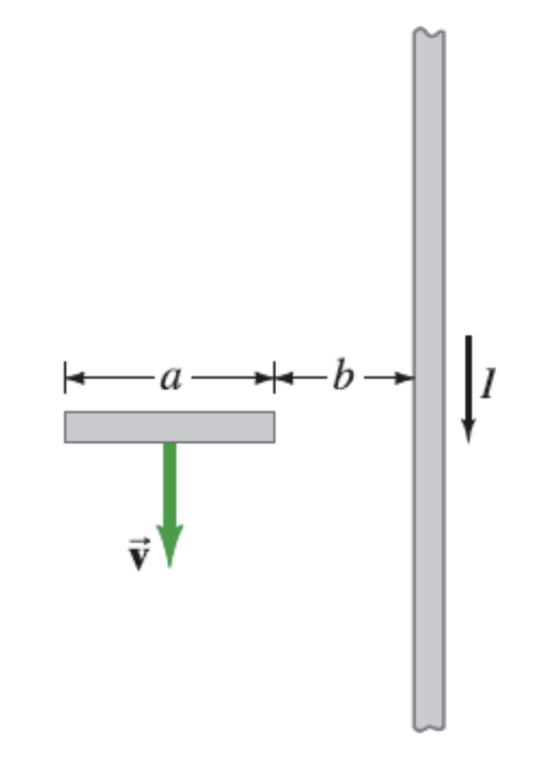
\includegraphics[scale = 0.28]{oz06/resources/Oz6Oef1.png}
    \end{minipage}

    \begin{enumerate}[(a)]
        \item     
            \begin{description}[labelwidth=1.5cm, leftmargin=!]
                \item[Geg. :] $v$, $I$, $a$, $b$
                \item[Gevr. :] $\mathcal{E}_{\text{ind}}$
                \item[Opl. :]
                \item[] 
                    \vspace{-0.45cm}\begin{minipage}{.6\textwidth}
                        Het magnetische veld van de lange draad gaat in het blad, maar het verkleint hoe verder we van de draad weggaan.
                        We berekenen de infinitesimale geïnduceerde emf 
                        \begin{equation*}
                            d\mathcal{E}_{\text{ind}} = B_{|}vdr = \frac{\mu_0vI}{2\pi r}dr
                        \end{equation*}
                        waarover we integreren tot we de volledige geïnduceerde emf hebben
                        \begin{equation*}
                            \mathcal{E}_{\text{ind}} = \int_{b}^{+b} \frac{\mu_0vI}{2\pi r}dr = \frac{\mu_0vI}{2\pi} \ln\left(\frac{b+a}{b}\right).
                        \end{equation*}
                        De emf is gericht \textbf{naar} de draad.
                    \end{minipage}
                    \hspace{0.5cm}\begin{minipage}{.36\textwidth}
                        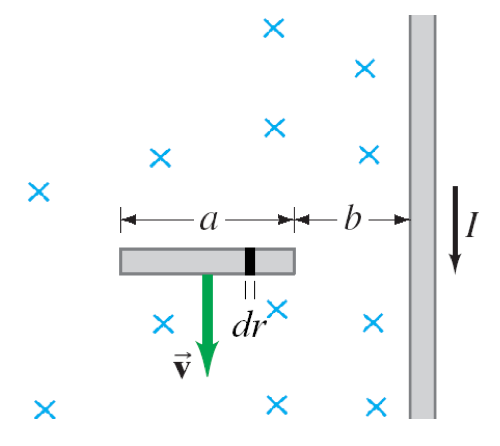
\includegraphics[scale = 0.4]{oz06/resources/Oz6Oef1-2.png}
                    \end{minipage}
            \end{description}
        \item     
            \begin{description}[labelwidth=1.5cm, leftmargin=!]
                \item[Geg. :] $v$, $I$, $a$, $b$
                \item[Gevr. :] $\mathcal{E}_{\text{ind}}$
                \item[Opl. :] Analoog aan (a), maar de emf is gericht \textbf{van} de draad.
            \end{description}
    \end{enumerate}

\vspace{1cm}

% \newpage

\phantomsection
\label{OZ6:2}
\textbf{\underline{OZ 6 - Magnetische inductie en de wet van Faraday - Oefening 2:}}
\vspace{0.5cm}

    \begin{minipage}{.79\textwidth}
        Een cirkelvormig circuit met straal $r$ bevat een weerstand $R$ en capaciteit $C$, en
        bevindt zich in een uniform magneetveld $\vec{B}$. Startend op tijdstip $t = 0$, begint het spanningsverschil $\Delta V = V_b - V_a$ over de condensator platen toe te nemen met tijd volgens $\Delta V = V_0 (1- e^{\frac{-t}{\tau}})$, met $V_0$ en $\tau$ positieve constanten. Bepaal $\frac{dB}{dt}$, de snelheid waarmee de grootte van het magnetisch veld verandert in functie van de tijd. Wordt $B$ groter of kleiner wanneer de tijd vordert?
    \end{minipage}
    \hspace{0.3cm}\begin{minipage}{.17\textwidth}
        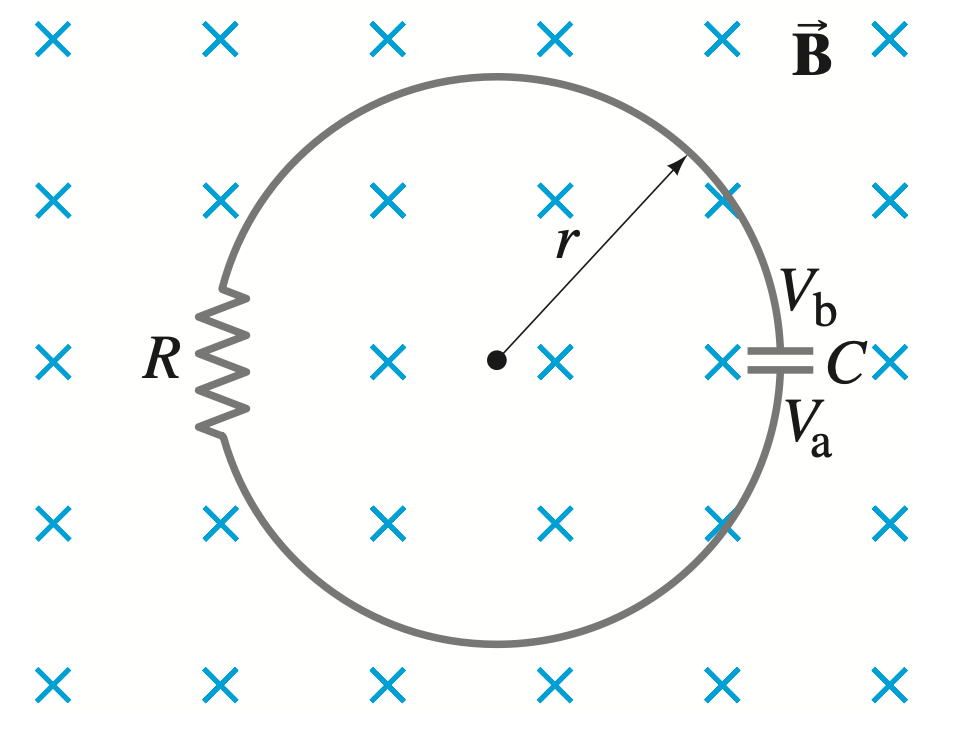
\includegraphics[scale = 0.23]{oz06/resources/Oz6Oef2.png}
    \end{minipage}

    \begin{description}[labelwidth=1.5cm, leftmargin=!]
        \item[Geg. :] $\vec{B}$, $R$, $C$, $r$, $V_0$, $\tau$
        \item[Gevr. :] $\frac{dB}{dt}$
        \item[Opl. :]
            Het magnetisch veld zal een emf induceren in het circuit, waardoor er een stroom tegen-wijzerzin zal lopen. De stroom kunnen we vinden met volgende formule 
            \begin{equation*}
                I = \frac{dQ}{dt} = \frac{d}{dt} \left(CV_0(1-e^{\frac{-t}{\tau}})\right) = \frac{V_0}{R}e^{\frac{-t}{\tau}}
            \end{equation*}
            waaruit we de geinduceerde emf kunnen vinden
            \begin{equation*}
                \mathcal{E}_{\text{ind}} = IR + V_C = V_0e^{\frac{-t}{\tau}} + V_0\left( 1 - e^{\frac{-t}{\tau}}\right) = V_0
            \end{equation*}
            wat we kunnen stoppen in de wet van faraday om de verandering van het magnetisch veld te vinden
            \begin{equation*}
                \frac{dB}{dt} = - \frac{\mathcal{E}_{\text{ind}}}{A} = - \frac{V_0}{\pi r^2}
            \end{equation*}
            en dus blijkt dat het magnetisch veld vermindert. Het geïnduceerde magnetische veld $\vec{B}_{\text{ind}}$ zal dus het magnetische veld $\vec{B}$ versterken en is dus in het bord gericht.

    \end{description}


\vspace{1cm}

\newpage

\phantomsection
\label{OZ6:3}
\textbf{\underline{OZ 6 - Magnetische inductie en de wet van Faraday - Oefening 3:}}
\vspace{0.5cm}

    \begin{minipage}{.7\textwidth}
        Een homogeen magnetisch veld wordt aangelegd in de cirkel. Het veld verandert in de tijd volgens $B = (2.00t3 - 4.00t2 +0.800) $ T met $t$ de tijd in seconden. Zij $r_2 = 2R = 5.00$ cm.

        \begin{enumerate}[(a)]
            \item Bereken de grootte en de richting van de kracht die inwerkt op een elektron dat zich in een punt $P_2$ bevindt als $t = 2.00$ s.
            \item Op welk tijdstip is deze kracht gelijk aan $0$?
        \end{enumerate}    
    \end{minipage}
    \hspace{0.5cm}\begin{minipage}{.2\textwidth}
        \includegraphics[scale = 0.22]{oz06/resources/Oz6Oef3.png}
    \end{minipage}

    \begin{enumerate}[(a)]
        \item     
            \begin{description}[labelwidth=1.5cm, leftmargin=!]
                \item[Geg. :]
                \item[Gevr. :] 
                \item[Opl. :]
            \end{description}
        \item     
            \begin{description}[labelwidth=1.5cm, leftmargin=!]
                \item[Geg. :]
                \item[Gevr. :] 
                \item[Opl. :]
            \end{description}
    \end{enumerate}



\vspace{1cm}

% \newpage

\phantomsection
\label{OZ6:4}
% \textbf{\underline{OZ 6 - Magnetische inductie en de wet van Faraday - Oefening 4:}}
% \vspace{0.5cm}

% Een rechthoekige loop met dimensies $ l $ en $ w $ beweegt met een constante snelheid $ v $ weg van een lange rechte draad waardoor een stroom $ I $ loopt, zoals aangeven op Figuur 6.4. De totale weerstand van de loop is $ R $. Bepaal een uitdrukking dat de stroom in de loop als een functie van de afstand $ r $.

% \begin{figure}[H]
%     \centering
%     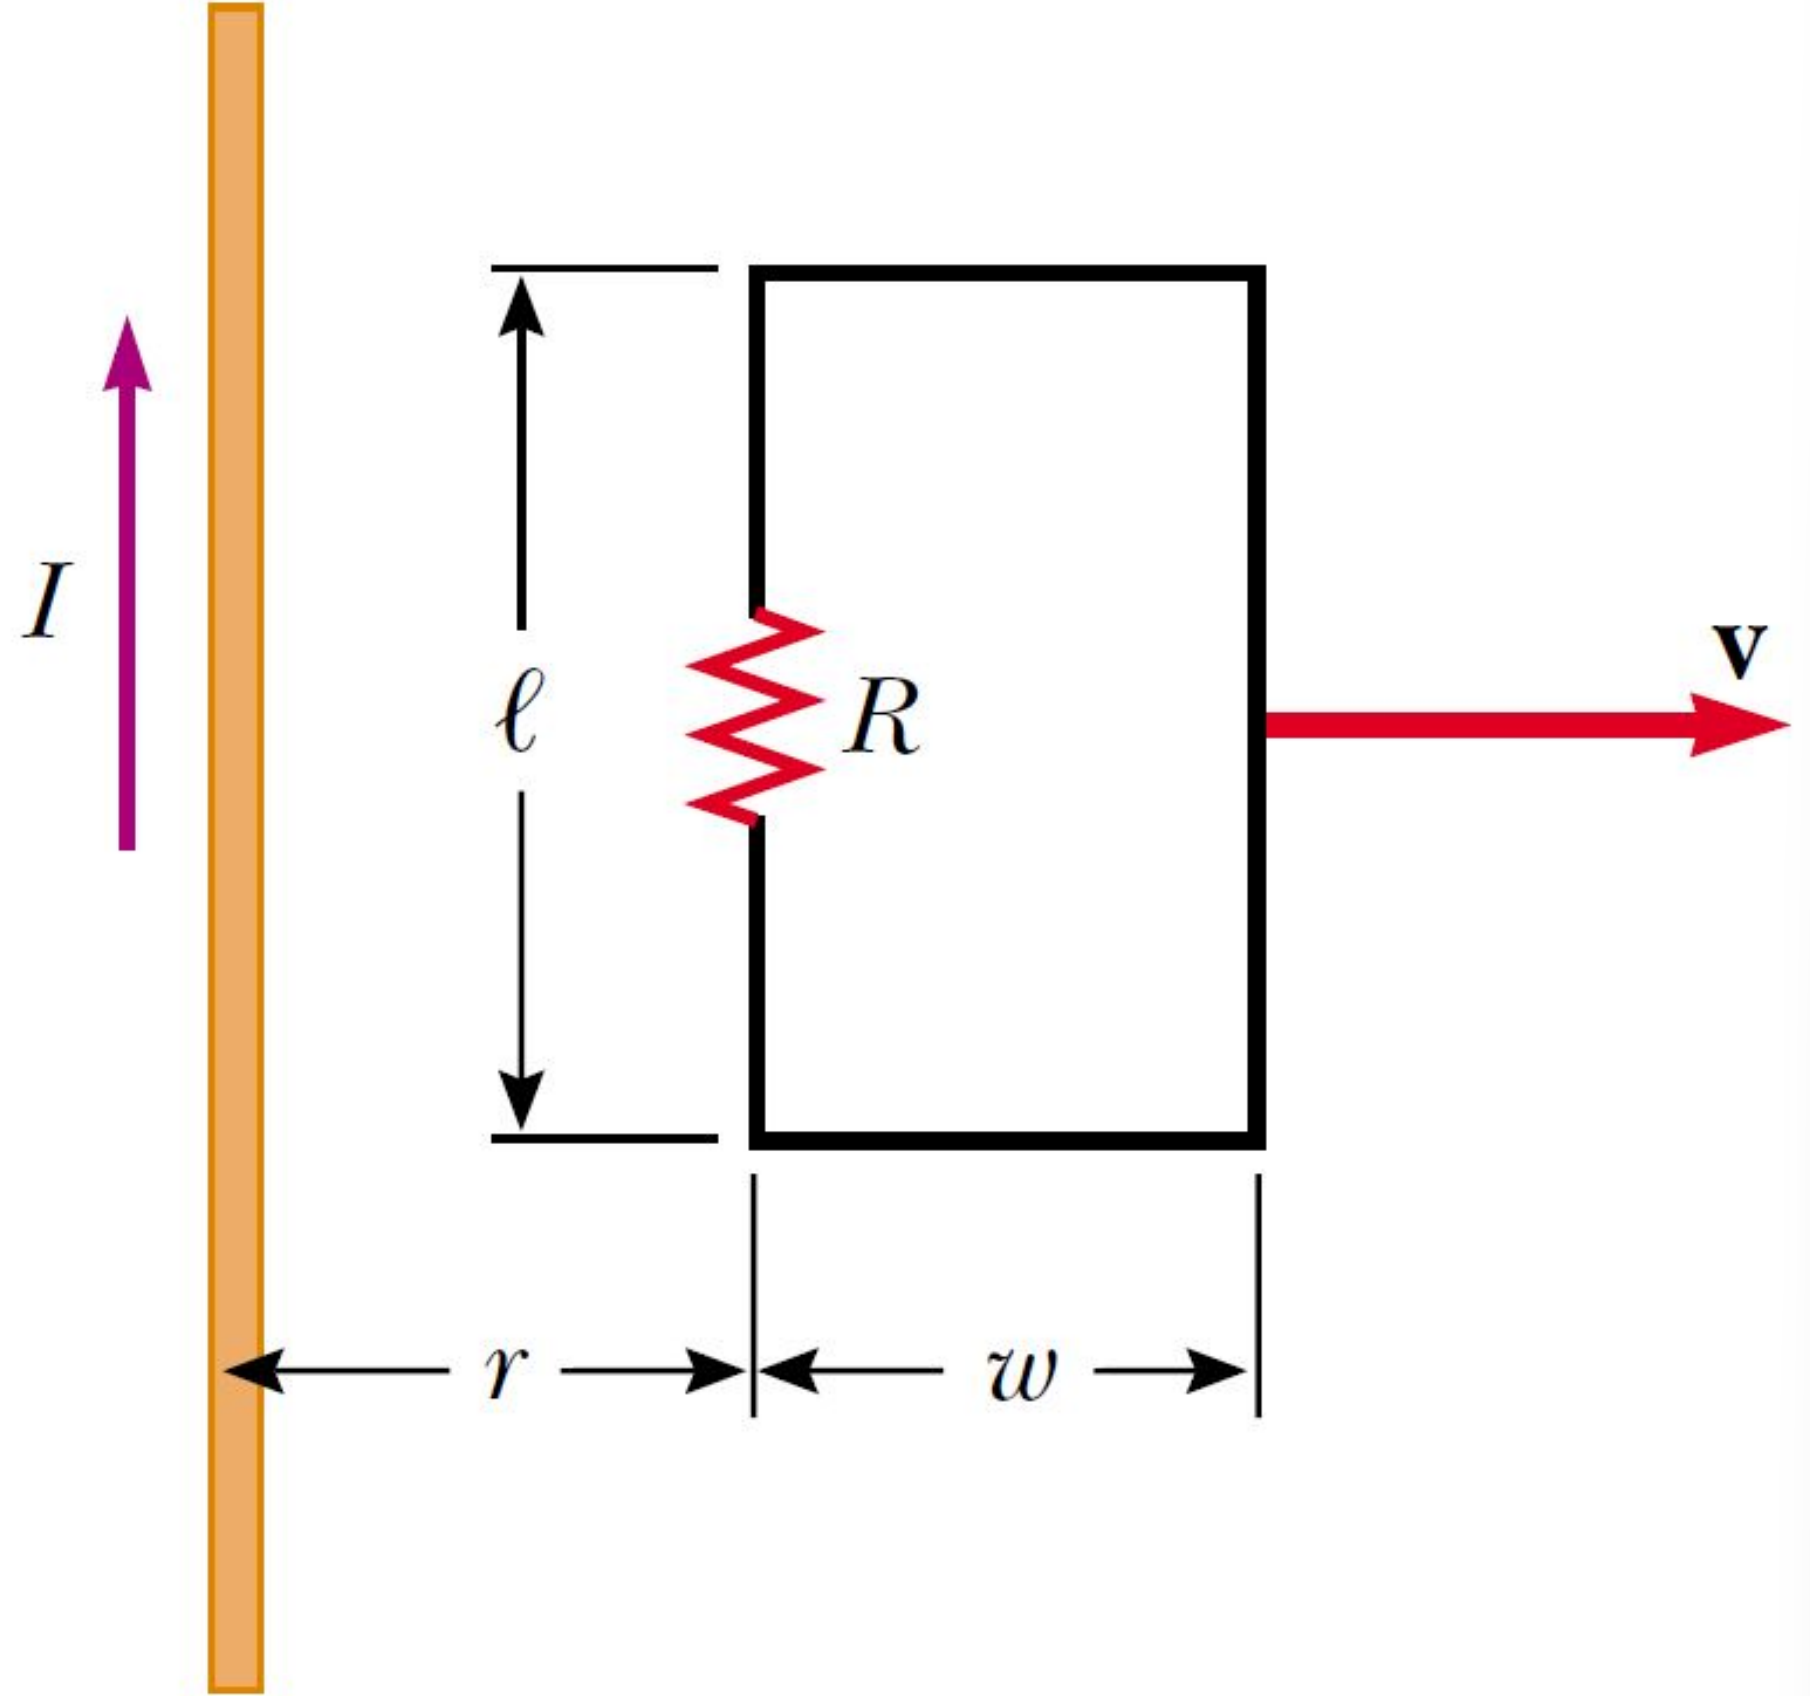
\includegraphics[width=5cm]{oz06/resources/oef-4-opgave.png}
    
%     \textbf{Figuur 6.4}
% \end{figure}

% \begin{description}[labelwidth=1.5cm, leftmargin=!]
%     \item[Geg. :]   $ l $; $ w $; $ v $; $ I $; $ R $;
%     \item[Gevr. :]  $ I_{l}(r) $;
%     \item[Opl. :]   $ B = \dfrac{\mu_0 I}{2 \pi r} $
                    
%                     $ \Phi_B = \int{\vec{B} \cdot d\vec{A}} = \int{\dfrac{\mu_0 I}{2 \pi r} \cdot l \cdot dr} $
                    
%                     \hspace{-0.57cm} $ \Rightarrow 
%                     \Phi_B = \dfrac{\mu_0 I l}{2 \pi} \int_{r}^{r+w}{\dfrac{dr}{r}} 
%                     = \dfrac{\mu_0 I l}{2 \pi} \left( \ln{\left| r+w \right|} - \ln{\left| r \right|} \right) 
%                     = \dfrac{\mu_0 I l}{2 \pi} \ln{\dfrac{r+w}{r}} 
%                     = \dfrac{\mu_0 I l}{2 \pi} \ln{\left( 1 + \dfrac{w}{r} \right)} $
                    
%                     \vspace{0.5cm}
                    
%                     $ r = r_0 + vt $
                    
%                     \vspace{0.5cm}
                    
%                     \hspace{-0.57cm} $ \Rightarrow 
%                     \Phi_B = \dfrac{\mu_0 I l}{2 \pi} \ln{\left( 1 + \dfrac{w}{r_0 + vt} \right)} $
                    
%                     \hspace{-0.57cm} $ \Rightarrow 
%                     \dfrac{d\Phi_B}{dt} = \dfrac{\mu_0 I l}{2 \pi} \dfrac{1}{1 + \dfrac{w}{r_0 + vt}} \dfrac{d}{dt}{\left( 1 + \dfrac{w}{r_0 + vt} \right)}
%                     = \dfrac{\mu_0 I l}{2 \pi} \dfrac{1}{1 + \dfrac{w}{r_0 + vt}} \dfrac{d}{dt}{\left( 1 + \dfrac{w}{r_0 + vt} \right)} $
                    
%                     \hspace{0.75cm} $ 
%                     = \dfrac{\mu_0 I l}{2 \pi} \dfrac{w}{1 + \dfrac{w}{r_0 + vt}} \dfrac{d}{dt}{\left( \dfrac{1}{r_0 + vt} \right)}
%                     = \dfrac{\mu_0 I l}{2 \pi} \dfrac{w}{1 + \dfrac{w}{r_0 + vt}} \dfrac{1}{\left( r_0 + vt \right)^2} \dfrac{d}{dt}{\left( r_0 + vt \right)}$
                    
%                     \hspace{0.75cm} $ 
%                     = \dfrac{\mu_0 I l}{2 \pi} \dfrac{w}{1 + \dfrac{w}{r_0 + vt}} \dfrac{v}{\left( r_0 + vt \right)^2}
%                     = \dfrac{\mu_0 I l}{2 \pi} \dfrac{w}{1 + \dfrac{w}{r}} \dfrac{v}{r^2} 
%                     = \dfrac{\mu_0 I l v}{2 \pi r} \dfrac{w}{r + w} $
                    
%                     $ \varepsilon = -\dfrac{d\Phi_B}{dt} = -\dfrac{\mu_0 I l v}{2 \pi r} \dfrac{w}{r + w} $
                    
%                     $ I = \dfrac{\varepsilon}{R} = -\dfrac{\mu_0 I l v}{2 \pi R r} \dfrac{w}{r + w} $
% \end{description}

% \vspace{1cm}

\newpage

\phantomsection
\label{OZ6:5}
\textbf{\underline{OZ 6 - Magnetische inductie en de wet van Faraday - Oefening 5:}}
\vspace{0.5cm}

    Twee oneindig lange solenoïdes gaan door een circuit zoals aangegeven. De grootte van het magnetisch veld in beide solenoïdes is hetzelfde en neemt toe met $100$ T/s. Welke stromen lopen er door verschillende weerstanden?

    \begin{center}
        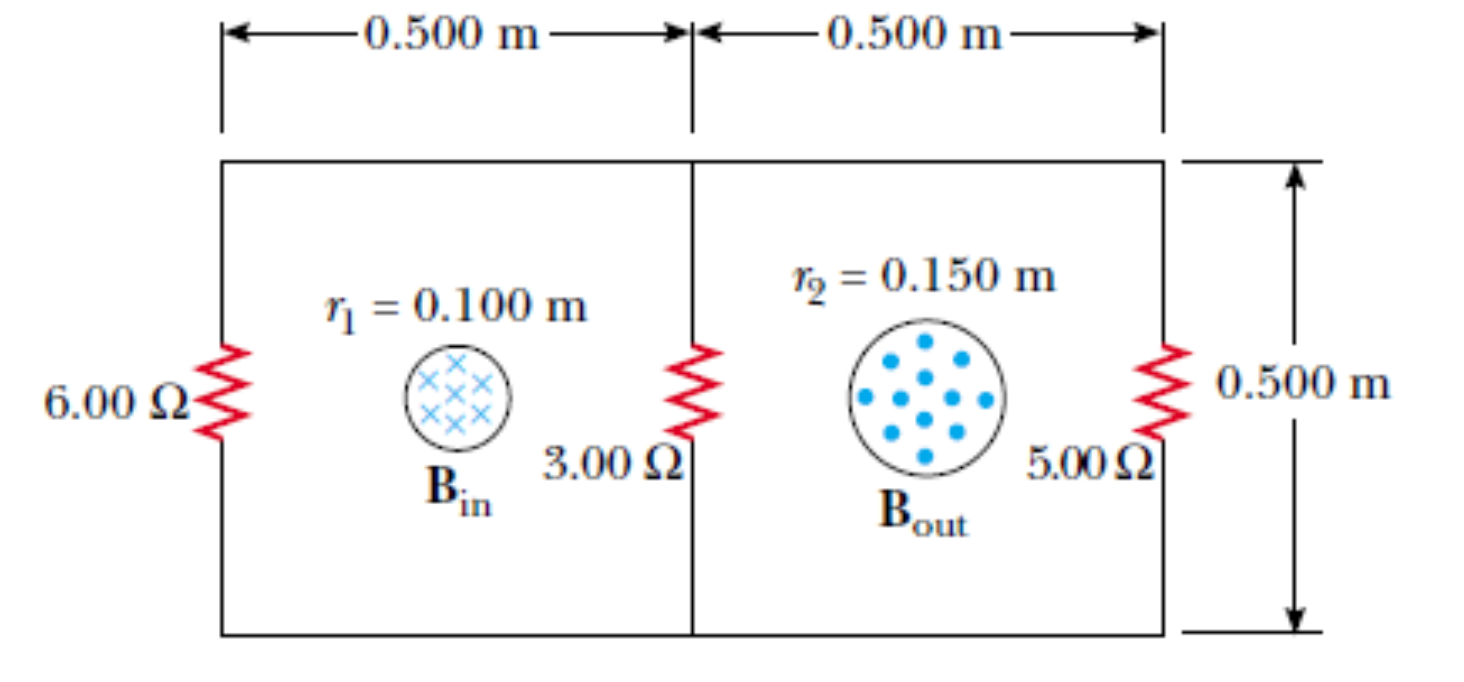
\includegraphics[scale = 0.3]{oz06/resources/Oz6Oef5.png}
    \end{center}

    \begin{description}[labelwidth=1.5cm, leftmargin=!]
        \item[Geg. :]
        \item[Gevr. :] 
        \item[Opl. :]
    \end{description}


\vspace{1cm}

\newpage

\pagebreak

\fakesection{Oefenzitting 7}

\phantomsection
\label{OZ7:1}
\textbf{\underline{OZ 7 - Inductantie - Oefening 1:}}
\vspace{0.5cm}

Bepaal voor de toroïde de energiedichtheid in het magnetisch veld in
functie van $r$ waarbij $r_1 < r < r_2$. Integreer dit over het volume om de totale energie
opgeslagen in de toroïde te vinden. De toroïde bevat $N$ windingen en draagt een
stroom $I$.

\begin{center}
    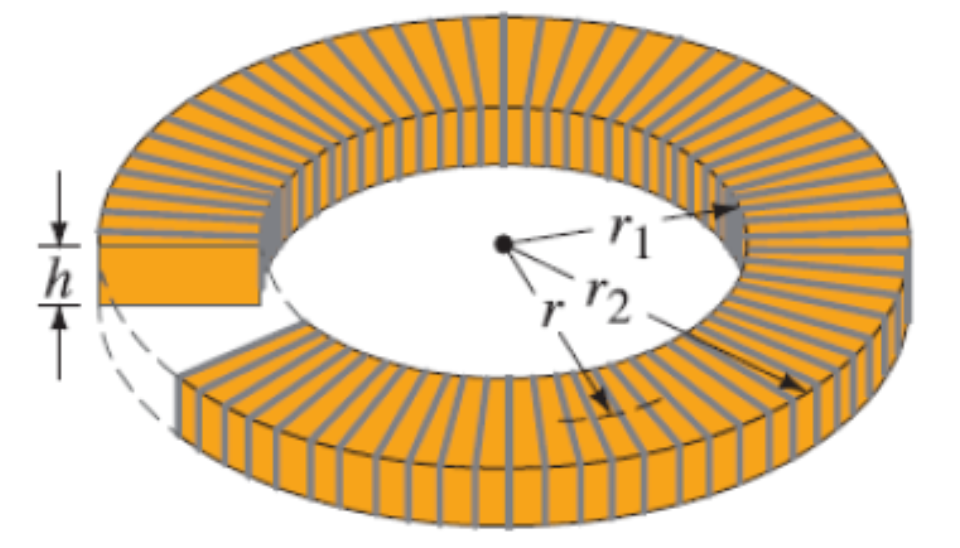
\includegraphics[scale = 0.3]{oz07/resources/Oz7Oef1.png}
\end{center}

\begin{description}[labelwidth=1.5cm, leftmargin=!]
    \item[Geg. :] 
    \item[Gevr. :] 
    \item[Opl. :]
\end{description}

\vspace{1cm}

\phantomsection
\label{OZ7:2}
\textbf{\underline{OZ 7 - Inductantie - Oefening 2:}}
\vspace{0.5cm}

Twee solenoïdes $A$ en $B$, die zich dicht in elkaars buurt bevinden en dezelfde cilindrische as delen, hebben $400$ en $700$ windingen, respectievelijk. Een stroom van $3.50$ A door spoel $A$ produceert een gemiddelde flux van $300$ $\mu$Wb door elke winding van $A$ en een flux van $90.0$ $\mu$Wb door elke winding van spoel B. 

\begin{enumerate}[(a)]
    \item Bereken de wederzijdse inductie van de twee solenoïdes.
    \item Wat is de zelfinductie van $A$?
    \item Welke emf wordt geïnduceerd in $B$ wanneer de stroom in $A$ stijgt met $0.500$ A/s
\end{enumerate}

% \begin{description}[labelwidth=1.5cm, leftmargin=!]
%     \item[Geg. :] 
%     \item[Gevr. :] 
%     \item[Opl. :]
% \end{description}

\begin{description}[labelwidth=1.5cm, leftmargin=!]
    \item[Geg. :] $N_A = 400$, $N_B = 700$, $I_A = 3.50$ A, $\Phi_{A} = 300$ $\mu$Wb, $\Phi_{B} = 90.0$ $\mu$Wb, 
\end{description}

\begin{enumerate}[(a)]
    \item 
        \begin{description}[labelwidth=1.5cm, leftmargin=!]
            \item[Gevr. :] $M_{BA}$ ?
            \item[Opl. :]  
                De wederzijdse inductie van twee spoelen wordt gegeven door:
                \begin{equation*}
                    M_{BA} = \frac{N_B \Phi_{BA}}{I_A}.
                \end{equation*}
                Er is geen stroom door B dus $\Phi_{BA} = \Phi_{B} = 90.0$ $\mu$Wb. De wederzijdse inductie wordt dan:
                \begin{equation*}
                    M_{BA} = \frac{N_B \Phi_{B}}{I_A} = 18.0 \ \text{mH}
                \end{equation*}

        \end{description}
    \item 
        \begin{description}[labelwidth=1.5cm, leftmargin=!] 
            \item[Gevr. :] $L_B$ ?
            \item[Opl. :]
                De zelfinductie van een spoel wordt gegeven door:
                \begin{equation*}
                    L_A = \frac{N_A \Phi_{A}}{I_A} = 34.3 \ \text{mH}
                \end{equation*}
        \end{description}
    \item
        \begin{description}[labelwidth=1.5cm, leftmargin=!]
            \item[Geg. :] $\frac{dI_A}{dt} = 0.500$ A/s
            \item[Gevr. :] $\mathcal{E}_B$ ?
            \item[Opl. :]
                De emf geïnduceerd in een spoel wordt gegeven door:
                \begin{equation*}
                    \mathcal{E}_B = -M_{BA} \frac{dI_A}{dt} = -9.00 \ \text{mV}
                \end{equation*}
        \end{description}
\end{enumerate}

\vspace{1cm}

\phantomsection
\label{OZ7:3}
\textbf{\underline{OZ 7 - Inductantie - Oefening 3:}}
\vspace{0.5cm}

Beschouw een circuit waarbij $ \mathcal{E} = 6,00 $ V, $ L = 8,00 $ mH, en $ R = 4,00 \ \Omega $.

\vspace{0.3cm}
\begin{minipage}{.75\textwidth}
    \begin{enumerate}[(a)]
        \item Wat is de inductieve tijdsconstante $ \tau $ van het circuit?
        \item Bereken de stroom in het circuit 250 $ \mu $s nadat de schakelaar gesloten werd.
        \item Wat is de uiteindelijke (steady-state) stroom?
        \item Hoe lang duurt het voordat de stroom 80 \% van zijn maximale waarde heeft bereikt?
    \end{enumerate}
\end{minipage}
\hspace{0.75cm}\begin{minipage}{.21\textwidth}
    \vspace{-0.5cm}\begin{center}
        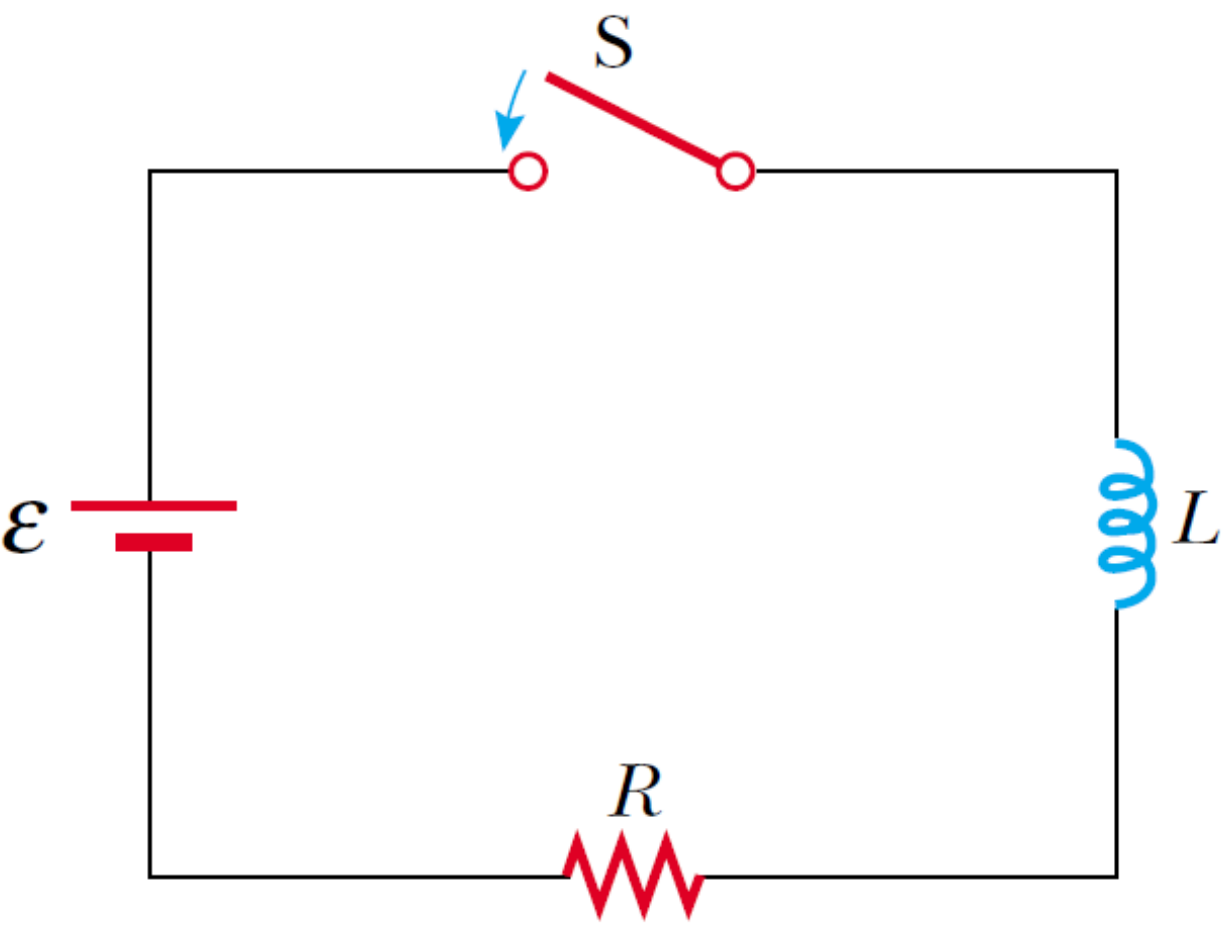
\includegraphics[scale = 0.28]{oz07/resources/oef-1-opgave.png}
    \end{center}
\end{minipage}

% \begin{description}[labelwidth=1.5cm, leftmargin=!]
%     \item[Geg. :] 
%     \item[Gevr. :] 
%     \item[Opl. :]
% \end{description}

\begin{description}[labelwidth=1.5cm, leftmargin=!]
    \item[Geg. :] $ \mathcal{E} = 6,00 $ V, $ L = 8,00 $ mH, $ R = 4,00 \ \Omega $
\end{description}

\begin{enumerate}[(a)]
    \item 
        \begin{description}[labelwidth=1.5cm, leftmargin=!]
            \item[Gevr. :] $\tau$
            \item[Opl. :]
                De inductieve tijdsconstante $ \tau $ van het circuit is gelijk aan
                \begin{equation*}
                    \tau = \frac{L}{R} = \frac{8,00 \cdot 10^{-3}}{4,00} = 2 \cdot 10^{-3} \ \text{s}
                \end{equation*}
        \end{description}
    \item 
        \begin{description}[labelwidth=1.5cm, leftmargin=!]
            \item[Geg. :] $t_1 = 250 \ \mu$s
            \item[Gevr. :] $I(t_1)$
            \item[Opl. :]
                We passen de wet van Kirchhoff toe op het circuit
                \begin{equation*}
                    \mathcal{E} = L \frac{\mathrm{d}I}{\mathrm{d}t} + RI
                \end{equation*}
                wat een differentiaalvergelijking is met oplossing
                \begin{equation*}
                    I(t) = \frac{\mathcal{E}}{R} \left(1 - e^{\frac{-t}{\tau}} \right)
                \end{equation*}
                waarin we de gegeven waarde invullen
                \begin{equation*}
                    I(t_1) = 0.176 \ \text{A}.
                \end{equation*}

        \end{description}
    \item 
        \begin{description}[labelwidth=1.5cm, leftmargin=!]
            \item[Gevr. :] $\lim_{t\to\infty} I(t)$
            \item[Opl. :]
                De steady-state stroom is gelijk aan
                \begin{equation*}
                    \lim_{t\to\infty} I(t) = \frac{\mathcal{E}}{R}\left(1 - \lim_{t\to\infty} e^{\frac{-t}{\tau}}\right) = \frac{\mathcal{E}}{R} = 1.50 \ \text{A}.
                \end{equation*}
        \end{description}
    \item 
        \begin{description}[labelwidth=1.5cm, leftmargin=!]
            \item[Gevr. :] $t_{80\%}$
            \item[Opl. :]
                De maximale stroom, of de steady-state stroom, is gelijk aan
                \begin{equation*}
                    I_{max} = \frac{\mathcal{E}}{R} = 1.50 \ \text{A}.
                \end{equation*}
                De stroom $I_{80\%}$ wordt dus eigenlijk gegeven door
                \begin{equation*}
                    I_{80\%} = \left(1 - e^{\frac{-t_{80\%}}{\tau}}\right) I_{max}.
                \end{equation*}
                We zoeken nu de tijd $t_{80\%}$ waarvoor
                \begin{equation*}
                   e^{\frac{-t_{80\%}}{\tau}} = 0.20
                \end{equation*}
                wat uitkomt op 
                \begin{equation*}
                    t_{80\%} = -\tau \ln(0.20) = 3.22 \cdot 10^{-3}\ \text{s}.
                \end{equation*}
        \end{description}
\end{enumerate}

% \begin{description}[labelwidth=1.5cm, leftmargin=!]
%     \item[Geg. :]   $ \varepsilon = 6,00 $ V; $ L = 8,00 $ mH; $ R = 4,00 \ \Omega $;
% \end{description}

% \begin{enumerate}[(a)]
%     \item 
%         \begin{description}[labelwidth=1.5cm, leftmargin=!]
%             \item[Gevr. :]  $ \tau $;
%             \item[Opl. :]   $ \tau = \dfrac{L}{R} = \dfrac{8,00 \cdot 10^{-3}}{4,00} = 0,00200 $ s
%         \end{description}
%     \item 
%         \begin{description}[labelwidth=1.5cm, leftmargin=!]
%             \item[Gevr. :]  $ I_{250 \mu\textrm{s}} $;
%             \item[Opl. :]   $ I = I_{max} \cdot \left(1 - e^{-t/\tau} \right) $ 
            
%                             $ I_{max} = \dfrac{\varepsilon}{R} = \dfrac{6,00}{5,00} = 1,50 $ A
                            
%                             $ I = 1,50 \cdot \left(1 - e^{-500t} \right) $ 
                            
%                             $ I_{250 \mu\textrm{s}} = 1,50 \cdot \left(1 - e^{-500 \cdot 250 \cdot 10^{-6}} \right) 
%                             = 0,17625 $ A $ \approx 0,176 $ A
%         \end{description}
%     \item 
%         \begin{description}[labelwidth=1.5cm, leftmargin=!]
%             \item[Gevr. :]  $ I_{250 \mu\textrm{s}} $;
%             \item[Opl. :]   $ I_{ss} = \lim_{t \to +\infty}{I_{max} \cdot \left(1 - e^{-t/\tau} \right)} = I_{max} 
%                             = 1,50 $ A
%         \end{description}
%     \item 
%         \begin{description}[labelwidth=1.5cm, leftmargin=!]
%             \item[Gevr. :]  $ t_{80 \%} $;
%             \item[Opl. :]   $ I = 0,80 \cdot I_{max} $
            
%                             \hspace{-0.57cm} $ \Leftrightarrow 
%                             I_{max} \cdot \left(1 - e^{-t_{80 \%}/\tau} \right) = 0,80 \cdot I_{max} $
            
%                             \hspace{-0.57cm} $ \Leftrightarrow 
%                             1 - e^{-t_{80 \%}/\tau} = 0,80 $
            
%                             \hspace{-0.57cm} $ \Leftrightarrow 
%                             e^{-t_{80 \%}/\tau} = 0,20 $
            
%                             \hspace{-0.57cm} $ \Leftrightarrow 
%                             -t_{80 \%}/\tau = \ln{0,20} $
            
%                             \hspace{-0.57cm} $ \Leftrightarrow 
%                             t_{80 \%} = - \ln{0,20} \cdot \tau = - \ln{0,20} \cdot 0,00200 = 0,0032189 $ s $ \approx 3,22 $ ms
%         \end{description}
% \end{enumerate}

\vspace{1cm}

\phantomsection
\label{OZ7:4}
\textbf{\underline{OZ 7 - Inductantie - Oefening 4:}}
\vspace{0.5cm}

Op $t = 0$ wordt de open schakelaar gesloten. Toon aan door de regels van Kirchhoff te gebruiken dat de stroom in de spoel op $t > 0$ gelijk is aan:

\begin{equation*}
    I(t) = \frac{\varepsilon}{R_1} \left( 1 - e^{-\tfrac{R'}{L}t} \right)
\end{equation*}

waarbij $R' = \frac{R_1R_2}{R_1 + R_2}$.

\begin{center}
    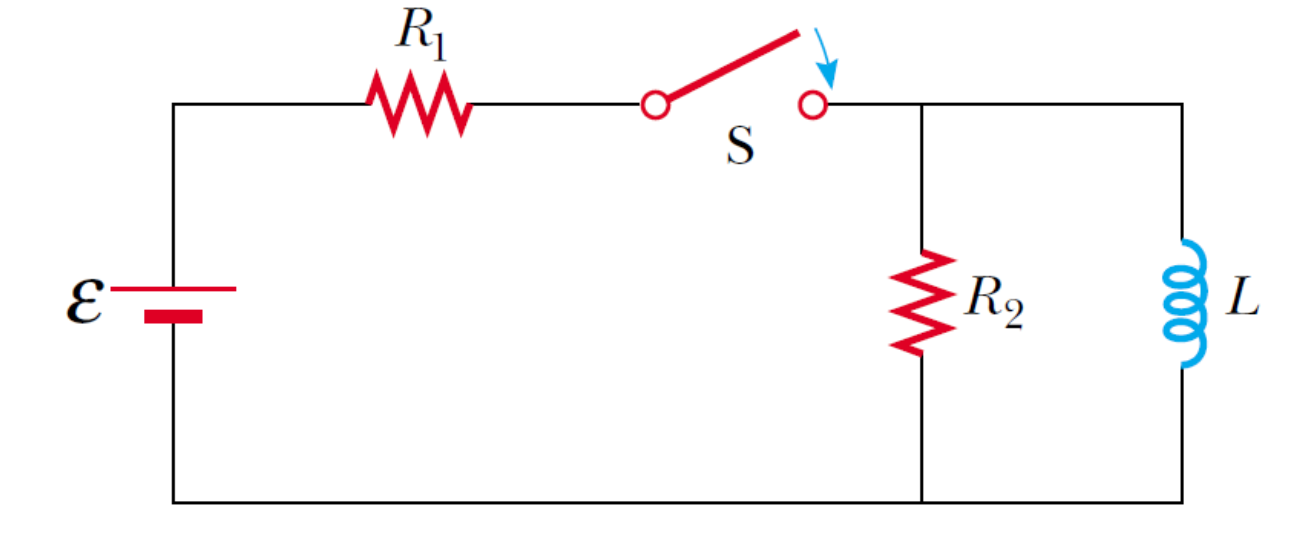
\includegraphics[scale = 0.3]{oz07/resources/Oz7Oef4.png}
\end{center}


\begin{description}[labelwidth=1.5cm, leftmargin=!]
    \item[Geg. :] 
    \item[Gevr. :] 
    \item[Opl. :]
\end{description}


\vspace{1cm}

\phantomsection
\label{OZ7:5}
\textbf{\underline{OZ 7 - Inductantie - Oefening 5:}}
\vspace{0.5cm}

Twee spoelen met zelfinductie $L_1$ en $L_2$ zijn parallel geschakeld. De wederzijdse inductie tussen de twee spoelen is $M$. Bepaal de equivalentie zelfinductie $L_{eq}$ van de twee spoelen.

\begin{center}
    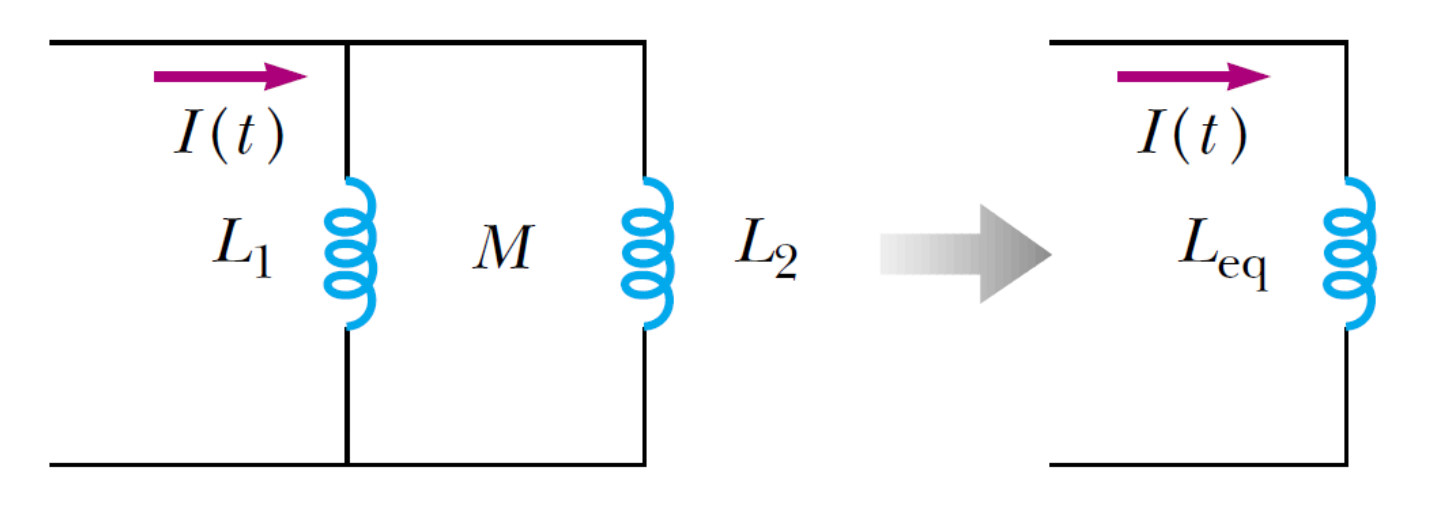
\includegraphics[scale = 0.3]{oz07/resources/Oz7Oef5.png}
\end{center}

\begin{description}[labelwidth=1.5cm, leftmargin=!]
    \item[Geg. :] $L_1$, $L_2$ en $M$
    \item[Gevr. :] $L_{eq}$ ? 
    \item[Opl. :]
        \begin{description}[labelwidth=1.5cm, leftmargin=!]
            \item[Gevr. :]  $L_{eq}$ ?
            \item[Opl. :]   
                Stel er is een spanningsbron $\mathcal{E}$. We krijgen de volgende spanningsvergelijkingen: 
                \begin{align}
                    \mathcal{E} 
                        &= - L_1 \frac{dI_1}{dt} - M \frac{dI_2}{dt} \tag{1} \\
                    \mathcal{E} 
                        &= - L_2 \frac{dI_2}{dt} - M \frac{dI_1}{dt} \tag{2} \\
                    \mathcal{E}
                        &= - L_{eq} \frac{dI}{dt}.  \tag{3}
                \end{align}
                met $I = I_1 + I_2$. Uit (1) vinden we
                \begin{equation*}
                    - \frac{dI_1}{dt} = \frac{\mathcal{E}}{L_1} + \frac{M}{L_1}\frac{dI_2}{dt}
                \end{equation*}
                wat we invullen in (2)
                \begin{equation*}
                    \mathcal{E} = - L_2 \frac{dI_2}{dt} + M \left(\frac{\mathcal{E}}{L_1} + \frac{M}{L_1}\frac{dI_2}{dt}\right) 
                \end{equation*}
                wat we herschrijven tot
                \begin{equation}
                    (-L_1L_2 + M^2)\frac{dI_2}{dt} = \mathcal{E}(L_1 - M) \tag{4}.
                \end{equation}
                Uit (2) vinden we
                \begin{equation*}
                    - \frac{dI_2}{dt} = \frac{\mathcal{E}}{L_2} + \frac{M}{L_2}\frac{dI_1}{dt}
                \end{equation*}
                wat we invullen in (1)
                \begin{equation*}
                    \mathcal{E} = - L_1 \frac{dI_1}{dt} + M \left(\frac{\mathcal{E}}{L_2} + \frac{M}{L_2}\frac{dI_1}{dt}\right)
                \end{equation*}
                wat we herschrijven tot
                \begin{equation}
                    (-L_1L_2 + M^2)\frac{dI_1}{dt} = \mathcal{E}(L_2 - M). \tag{5}
                \end{equation}
                Als we (4) en (5) optellen vinden we
                \begin{equation*}
                    (-L_1L_2 + M^2)\left(\frac{dI_1}{dt} + \frac{dI_2}{dt}\right) = \mathcal{E}(L_1 + L_2 - 2M)
                \end{equation*}
                sinds (3) geldt, volgt
                \begin{equation*}
                    L_{eq} = - \frac{-L_1L_2 + M^2}{L_1 + L_2 - 2M} = \frac{L_1L_2 - M^2}{L_1 + L_2 - 2M}
                \end{equation*}
        \end{description}
\end{description}

\vspace{1cm}

\newpage

\pagebreak

\fakesection{Oefenzitting 8}

\phantomsection
\label{OZ8:1}
\textbf{\underline{OZ 8 - LC- en  RLC-circuits - Oefening 1:}}
\vspace{0.5cm}

Op $t = 0$ s wordt een emf van $500$ V aangelegd op een spoel met een inductantie van
$0.800$ H en een weerstand $30 \ \Omega$.

\begin{enumerate}[(a)]
    \item Bepaal de energie opgeslagen in het magnetisch
    veld wanneer de stroom de helft van zijn maximale waarde heeft bereikt
    \item Nadat de emf wordt aangesloten, hoe lang duurt het voordat de helft van de maximale
    stroom bereikt wordt?
\end{enumerate}

\begin{description}[labelwidth=1.5cm, leftmargin=!]
    \item[Geg. :]  $L = 0.800 \ \text{H}$, $R = 30 \ \Omega$, $V = 500 \ \text{V}$
\end{description}

\begin{enumerate}[(a)]
    \item 
        \begin{description}[labelwidth=1.5cm, leftmargin=!]
            \item[Geg. :] $I = \frac{1}{2}I_{\text{max}}$
            \item[Gevr. :] $U_L$ ?
            \item[Opl. :]  
                De maximale stroom is triviaal te berekenen:
                \begin{equation*}
                    I_{\text{max}} = \frac{V}{R}
                \end{equation*}
                Als we nu de energie willen berekenen op het moment dat de stroom de helft van zijn maximale waarde heeft bereikt, dan gebruiken we de volgende formule:
                \begin{equation*}
                    U_L = \frac{1}{2} L I^2 = \frac{1}{2}L\left(\frac{1}{2} I_{\text{max}}\right)^2 =  \frac{1}{8}\frac{LV^2}{R^2} = 27.8 \ \text{J}.
                \end{equation*}
        \end{description}
    \item 
        \begin{description}[labelwidth=1.5cm, leftmargin=!]
            \item[Gevr. :] $t_{50\%}$ ?
            \item[Opl. :]   
                De stroom in een RL-kring is gegeven door:
                \begin{equation*}
                    I(t) = I_{\text{max}}\left(1 - e^{-\frac{R}{L}t}\right)
                \end{equation*}
                We zoeken nu de tijd $t_{50\%}$ (na een paar triviale herwerkingsstappen) waarvoor geldt dat 
                \begin{equation*}
                    e^{-\frac{R}{L}t_{50\%}} = \frac{1}{2}
                \end{equation*}
                wat we makkelijk oplossen door het natuurlijke logaritme te nemen van beide kanten:
                \begin{equation*}
                    t_{50\%} = -\frac{L}{R}\ln\left(\frac{1}{2}\right) = 18.5 \ \text{ms}.
                \end{equation*}
        \end{description}
\end{enumerate}



\vspace{1cm}

\phantomsection
\label{OZ8:2}
\textbf{\underline{OZ 8 - LC- en  RLC-circuits - Oefening 2:}}
\vspace{0.5cm}

Een spoel met $820$ windingen heeft een weerstand van $24,0 \ \Omega$, en wordt geplaatst rond een solenoïde met $12500$ windingen van $7.00$ cm lang. Zowel de spoel als de solenoïde hebben een doorsnede van oppervlakte $1.00\cdot10^{-4} \ \text{m}^2$.

\vspace{0.3cm}
\begin{minipage}{.66\textwidth}
    \begin{enumerate}[(a)]
        \item 
            Hoe lang duurt het voordat de stroom door de solenoïde $63,2\%$ van zijn maximale waarde bereikt?
        \item 
            Bepaal de gemiddelde tegen-emf veroorzaakt door de zelfinductie van de solenoïde tijdens dit tijdsinterval,
        \item 
            de gemiddelde snelheid van verandering van het magnetische flux door de spoel tijdens dit tijdsinterval,
        \item 
            en de grootte van de gemiddelde geïnduceerde stroom in de spoel.
    \end{enumerate}
\end{minipage}
\begin{minipage}{.3\textwidth}
    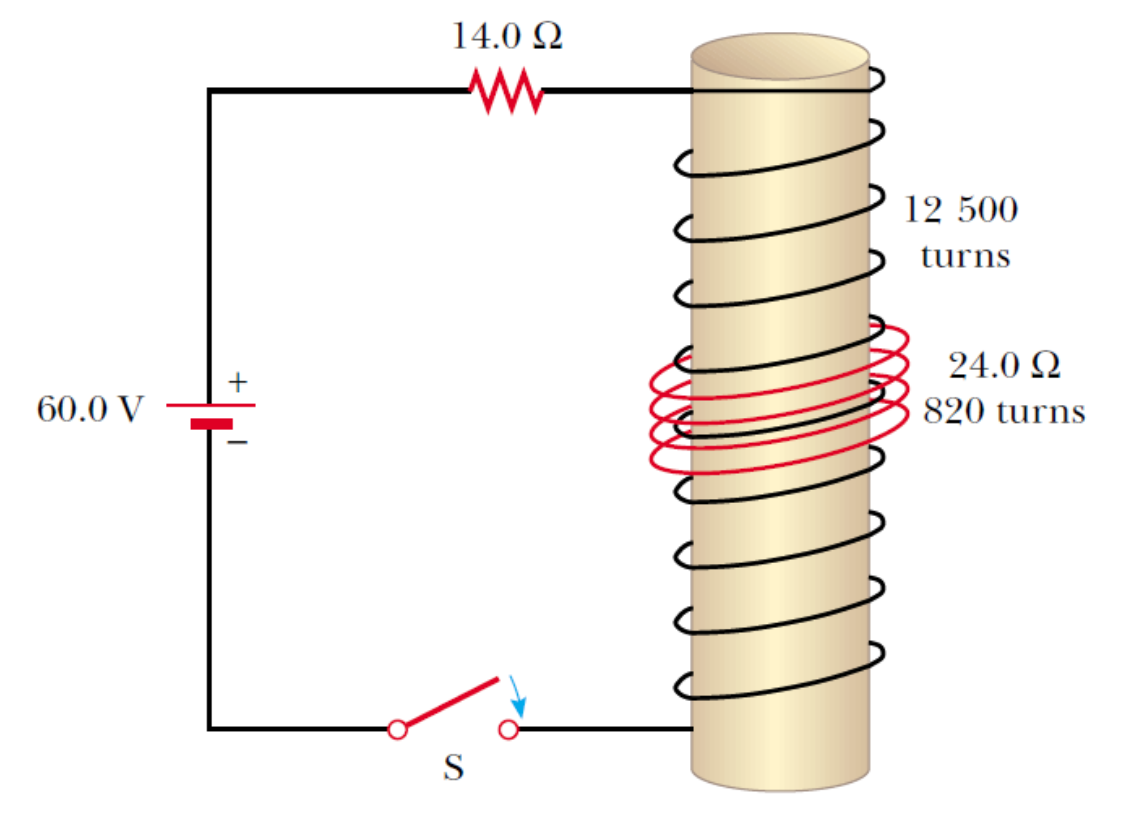
\includegraphics[scale = 0.3]{oz08/resources/Oz8Oef2.png}
\end{minipage}

\begin{description}[labelwidth=1.5cm, leftmargin=!]
    \item[Geg. :]   $N_{\text{spoel}} = 820$, $R_{\text{spoel}} = 24.0 \ \Omega$, $N_{\text{sol}} = 12500$, $\ell_{\text{sol}} = 7.00 \ \text{cm}$, $A_{\text{spoel}} = A_{\text{sol}} = 1.00\cdot10^{-4} \ \text{m}^2$, $R = 14.0 \ \Omega$, $\mathcal{E} = 60 \ \text{V}$
\end{description}

\begin{enumerate}[(a)]
    \item 
        \begin{description}[labelwidth=1.5cm, leftmargin=!]
            \item[Gevr. :] $t_{63.2\%}$ ?
            \item[Opl. :]  
                De tweede wet van Kirchhoff geeft ons volgende vergelijking:
                \begin{equation*}
                    \mathcal{E} = I_{{\text{sol}}}R + L\frac{dI_{{\text{sol}}}}{dt} .
                \end{equation*}
                % Met de wet van Faraday vinden we:
                % \begin{align}
                %     \left|\mathcal{E}_{\text{back}}\right| &=
                %     L_{\text{sol}}\frac{dI_{\text{sol}}}{dt} = N_{\text{sol}}\frac{d}{dt}\left(AB_{\text{sol}}\right) = \frac{\mu_0N_{\text{sol}}^2A}{\ell_{\text{sol}}}\frac{dI_{\text{sol}}}{dt} \\
                %     %
                %     \left|\mathcal{E}_{\text{ind}}\right| &= M\frac{dI_{\text{spoel}}}{dt} = N_{\text{sol}}\frac{d}{dt}\left(AB_{\text{spoel}}\right) = \frac{\mu_0N_{\text{sol}}N_{\text{spoel}}A}{\ell_{\text{spoel}}}\frac{dI_{\text{sol}}}{dt}
                % \end{align}
                % Als we (1) en (2) invullen in de vergelijking van Kirchhoff vinden we:
                % \begin{equation*}
                %     \mathcal{E} = I_{{\text{sol}}}R + \mu_0A\left(\frac{N_{\text{sol}}^2}{\ell_{\text{sol}}} + \frac{N_{\text{sol}}N_{\text{spoel}}}{\ell_{\text{spoel}}} \right)\frac{dI_{\text{sol}}}{dt}.
                % \end{equation*}
                % Stel nu dat
                % \begin{equation*}
                %     L_{\text{eq}} = \mu_0A\left(\frac{N_{\text{sol}}^2}{\ell_{\text{sol}}} + \frac{N_{\text{sol}}N_{\text{spoel}}}{\ell_{\text{spoel}}}\right)
                % \end{equation*}
                % dan vinden we voor de stroom door de solenoïde
                % \begin{equation*}
                %     I_{\text{sol}}(t) = \frac{\mathcal{E}}{R} \left( 1 - e^{-\frac{R}{L_{\text{eq}}}t} \right).
                % \end{equation*}
                % We bewijzen nu dat we kunnen aannemen dat dit equivalent is aan de formule van een RL-kring: 
                % \begin{tcolorbox}
                %     \begin{description}
                %         \item[T.B. :] $\frac{d}{dt} I_{\text{spoel}}(t) << \frac{d}{dt} I_{\text{sol}}(t)$
                %         \item[Aanname :] $N_{\text{sol}} << N_{\text{spoel}}$
                %         \item[B. :] 
                %             We kunnen deze constructie zien als een transformator en dus:
                %             \begin{equation*}
                %                 I_{\text{sol}}(t) = \frac{N_{\text{spoel}}}{N_{\text{sol}}} I_{\text{spoel}}(t).
                %             \end{equation*}
                %             Dit kunnen we afleiden
                %             \begin{equation*}
                %                 \frac{d}{dt} I_{\text{sol}}(t) = \frac{N_{\text{spoel}}}{N_{\text{sol}}} \frac{d}{dt} I_{\text{spoel}}(t)
                %             \end{equation*}
                %             en dankzij onze aanname volgt dat 
                %             \begin{equation*}
                %                 \frac{d}{dt} I_{\text{spoel}}(t) << \frac{d}{dt} I_{\text{sol}}(t).
                %             \end{equation*}
                %     \end{description}
                % \end{tcolorbox}
                % Er is dus bewezen dat we van een RL-kring mogen spreken. 
                In een RL-kring volgt de stroom de volgende formule:
                \begin{equation*}
                    I(t) = I_{\text{max}} \left( 1 - e^{-\frac{t}{\tau}} \right)
                \end{equation*}
                met $\tau = \frac{L}{R}$. De stroom bereikt $63.2\%$ van zijn maximale waarde wanneer $t = \tau $. We kunnen dus stellen dat
                \begin{equation*}
                    t_{63.2\%} = \frac{L_{{\text{sol}}}}{R} = \frac{\mu_0N_{{\text{sol}}}^2A_{{\text{sol}}}}{\ell_{{\text{sol}}}R}.
                \end{equation*}
                We berekenen nu triviaal de tijd door in te vullen:
                \begin{equation*}
                    t_{63.2\%} = 0.02 \ \text{s} \approx 20.0 \ \text{ms}.
                \end{equation*}
        \end{description}
        \newpage
    \item 
        \begin{description}[labelwidth=1.5cm, leftmargin=!]
            \item[Gevr. :] $\mathcal{E}_{\text{back}}$ ?
            \item[Opl. :]
                De gemiddelde geïnduceerde emf is gelijk aan 
                \begin{equation*}
                    \mathcal{E}_{\text{back}} = -L_2 \frac{\Delta I}{\Delta t}.
                \end{equation*}
                waarbij 
                \begin{equation*}
                    \frac{\Delta I}{\Delta t} = 0.632 \frac{\Delta I_{\text{max}}}{\Delta t} = 0.632 \frac{\Delta V}{R\Delta t}.
                \end{equation*}
                We kunnen nu de geïnduceerde emf berekenen:
                \begin{equation*}
                    \mathcal{E}_{\text{back}} = -L_2 \frac{\Delta I}{\Delta t} = -0.632 \frac{\mu_0N_2^2A_2}{\ell_{{\text{sol}}}}\frac{\Delta V}{R\Delta t} = -37.9 \ \text{V}.
                \end{equation*}
        \end{description}
    \item 
        \begin{description}[labelwidth=1.5cm, leftmargin=!]
            \item[Gevr. :] $\frac{\Delta \Phi_B}{\Delta t}$ ?
            \item[Opl. :]   
                De gemiddelde snelheid van de verandering van het magnetische flux is gelijk aan 
                \begin{equation*}
                    \frac{\Delta \Phi_B}{\Delta t} = -\frac{\mathcal{E}_{\text{back}}}{N_{{\text{sol}}}} \approx 3.04 \ \text{mV}.
                \end{equation*}
        \end{description}
    \item 
        \begin{description}[labelwidth=1.5cm, leftmargin=!]
            \item[Gevr. :] $I_{\text{ind}}$ ?
            \item[Opl. :]   
                De gemiddelde stroom is gelijk aan 
                \begin{equation*}
                    I_{\text{ind}} = \frac{\mathcal{E}_{\text{ind}}}{R_{{\text{spoel}}}} = \frac{N_{{\text{spoel}}}}{R_{{\text{spoel}}}}\frac{\Delta \Phi_B}{\Delta t} \approx 104 \ \text{mA}.
                \end{equation*}
        \end{description}
\end{enumerate}

\textbf{Opmerking:} in (b), (c) en (d) wordt er gevraagd achter het gemiddelde en niet ogenblikkelijke! 

\vspace{1cm}

\newpage

\phantomsection
\label{OZ8:3}
% \textbf{\underline{OZ 8 - $ LC $- en $ RLC $-circuits - Oefening 3:}}
% \vspace{0.5cm}

% Beschouw een $ LC $-circuit bestaande uit een parallelle-platen condensator met oppervlakte $ A $ en een spoel met inductantie $ L $. Dit circuit kan op de volgende manier gebruikt worden om kleine afstanden te bepalen:

% \begin{enumerate}[(a)]
%     \item Indien een lading in dit circuit oscilleert met frequentie $ f $ als de platen van de condensator zich op een afstand $ x $ van elkaar bevinden, toon dan aan dat $ x = 4 \pi^2 A \varepsilon_0 f^2 L $.
%     \item Wanneer we de afstand aanpassen met $ \Delta x $, verandert de frequentie met $ \Delta f $. Toon aan dat $ \Delta x/x \approx 2 \left( \Delta f/f \right) $.
% \end{enumerate}

% \begin{description}[labelwidth=1.5cm, leftmargin=!]
%     \item[Geg. :]   $ A $; $ L $;
% \end{description}

% \begin{enumerate}[(a)]
%     \item 
%         \begin{description}[labelwidth=1.5cm, leftmargin=!]
%             \item[Geg. :]   $ f $; $ x $;
%             \item[Gevr. :]  Toon aan dat $ x = 4 \pi^2 A \varepsilon_0 f^2 L $;
%             \item[Opl. :]   $ C = \dfrac{\varepsilon_0 A}{x} $
            
%                             $ I X_C = I X_L $
                            
%                             \hspace{-0.57cm} $ \Leftrightarrow 
%                             \dfrac{1}{\omega C} = \omega L $
                            
%                             \hspace{-0.57cm} $ \Leftrightarrow 
%                             C = \dfrac{1}{\omega^2 L} $
                            
%                             \hspace{-0.57cm} $ \Leftrightarrow 
%                             \dfrac{\varepsilon_0 A}{x} = \dfrac{1}{\omega^2 L} $
                            
%                             \hspace{-0.57cm} $ \Leftrightarrow
%                             x = \varepsilon_0 A \omega^2 L 
%                             = \varepsilon_0 A (2 \pi f)^2 L 
%                             = 4 \pi^2 A \varepsilon_0 f^2 L $
%         \end{description}
%     \item
%         \begin{description}[labelwidth=1.5cm, leftmargin=!]
%             \item[Geg. :]   $ x $; $ \Delta x $; $ f $; $ \Delta f$;
%             \item[Gevr. :]  Toon aan dat $ \Delta x/x \approx 2 \left( \Delta f/f \right) $;
%             \item[Opl. :]   $ \dfrac{\Delta x}{x} = \dfrac{x_e - x}{x} 
%                             = \dfrac{4 \pi^2 A \varepsilon_0 f_e^2 L - 4 \pi^2 A \varepsilon_0 f^2 L}{4 \pi^2 A \varepsilon_0 f^2 L}
%                             = \dfrac{f_e^2 - f^2}{f^2}
%                             = \dfrac{\left( f_e - f \right) \left( f_e + f \right)}{f^2} $
                            
%                             \vspace{0.5cm}
                            
%                             \begin{quote}
%                                 Kleine verandering $ \to f_e + f \approx 2f $
%                             \end{quote}
                            
%                             \vspace{0.5cm}
                            
%                             $ \dfrac{\Delta x}{x} \approx \dfrac{\left( f_e - f \right) 2f}{f^2} = 2 \dfrac{f_e - f}{f} $
                            
%                             \hspace{-0.57cm} $ \Rightarrow
%                             \dfrac{\Delta x}{x} \approx 2 \dfrac{\Delta f}{f} $
%         \end{description}
% \end{enumerate}

% \vspace{1cm}

\phantomsection
\label{OZ8:4}
\textbf{\underline{OZ 8 - LC- en  RLC-circuits - Oefening 4:}}
\vspace{0.5cm}

Beschouw de kring met een spanningsbron met emf van $50.0 \ \text{V}$, een weerstand van $250 \ \Omega$, en een capaciteit van $0.500 \ \mu \text{F}$. De schakelaar S is gesloten voor een lange tijd en geen spanningsverschil wordt gemeten over de condensator. Nadat de schakelaar geopend wordt, bereikt het potentiaal verschil over de condensator een maximale waarde van $150.0 \ \text{V}$. Wat is dan de inductantie $L$ in de kring?

\begin{center}
    \includegraphics[scale = 0.3]{oz08/resources/Oz8Oef4.png}
\end{center}
    
\begin{description}[labelwidth=1.5cm, leftmargin=!]
    \item[Geg. :]  $\mathcal{E} = 50.0 \ \text{V}$, $R = 250 \ \Omega$, $C = 0.500 \ \mu \text{F}$, $\Delta V_{\text{max}} = 150.0 \ \text{V}$
    \item[Gevr. :] $L$ ?
    \item[Opl. :] 
        Stel de schakelaar is lang gesloten geweest, dan is de stroom 
        \begin{equation*}
            I_{\text{max}} = \frac{\mathcal{E}}{R}
        \end{equation*}
        want de condensator is dan volledig opgeladen. Eens we de schakelaar openen, dan zal de linkse lus een open circuit zijn en het rechtse een LC-kring. De energie in de kring is behouden, dus
        \begin{equation*}
            \frac{1}{2}LI_{\text{max}}^2 = \frac{1}{2}C\Delta V_{\text{max}}^2. 
        \end{equation*}
        We kunnen nu de inductantie berekenen:
        \begin{equation*}
            L = \frac{C\Delta V_{\text{max}}^2}{I_{\text{max}}^2} = \frac{C\Delta V_{\text{max}}^2R^2}{\mathcal{E}^2} \approx 281 \ \text{mH}.
        \end{equation*}

\end{description}

\vspace{1cm}

\newpage

\phantomsection
\label{OZ8:5}
\textbf{\underline{OZ 8 - LC- en  RLC-circuits - Oefening 5:}}
\vspace{0.5cm}

Beschouw een LC-kring waarbij $L = 500 \ \text{mH}$ en $C = 0.100 \ \mu \text{F}$. 

\begin{enumerate}[(a)]
    \item 
        Wat is de resonantie frequentie $\omega_0$?
    \item 
        Indien een weerstand R van $1.00 \ \text{k}\Omega$ wordt toegevoegd aan het circuit, wat is dan de frequentie van de (gedempte) oscillaties?
\end{enumerate}

\begin{description}[labelwidth=1.5cm, leftmargin=!]
    \item[Geg. :]   $L = 500 \ \text{mH}$, $C = 0.100 \ \mu \text{F}$
\end{description}

\begin{enumerate}[(a)]
    \item 
        \begin{description}[labelwidth=1.5cm, leftmargin=!]
            \item[Gevr. :] $\omega_0$ ?
            \item[Opl. :]   
                De resonantie frequentie in een LC-kring wordt gegeven door de volgende formule:
                \begin{equation*}
                    \omega_0 = \frac{1}{\sqrt{LC}} \approx 4.47 \cdot 10^3 \ \text{rad/s}.
                \end{equation*}
        \end{description}
    \item 
        \begin{description}[labelwidth=1.5cm, leftmargin=!]
            \item[Geg. :]   $R = 1.00 \ \text{k}\Omega$
            \item[Gevr. :] $\omega$ ?
            \item[Opl. :]   
                De frequentie van de gedempte oscillaties wordt gegeven door de volgende formule:
                \begin{equation*}
                    \omega = \sqrt{\omega_0^2 - \frac{R^2}{4L^2}} \approx 4.36 \cdot 10^3 \ \text{rad/s}.
                \end{equation*}
        \end{description}
\end{enumerate}

\vspace{1cm}

\newpage

\pagebreak

\fakesection{Oefenzitting 9}

\phantomsection
\label{OZ9:1}
\textbf{\underline{OZ 9 - Wisselstroomkringen - Oefening 1:}}
\vspace{0.5cm}

Bereken $Z$, $X_L$, $X_C$ en $\phi$ voor een AC-circuit met $R = 300 \ \Omega$, $C = 11.0 \ \mu\text{F}$, $L = 0,200 \ \text{H}$, en $f = (500/\pi) \ \text{Hz}$. Teken het bijhorende fasordiagram.

% \begin{enumerate}[(a)]
%     \item #
% \end{enumerate}

\begin{description}[labelwidth=1.5cm, leftmargin=!]
    \item[Geg. :]  $R = 300 \ \Omega$, $C = 11.0 \ \mu\text{F}$, $L = 0,200 \ \text{H}$, $f = (500/\pi) \ \text{Hz}$ 
    \item[Gevr. :] $Z$, $X_L$, $X_C$, $\phi$ ?
    \item[Opl. :]   
        We berekenen $\omega$:
        \begin{equation*}
            \omega = 2\pi f = 1000 \ \text{rad/s}
        \end{equation*}
        We berekenen $X_L$ en $X_C$:
        \begin{align*}
            X_L &= \omega L \approx 200 \ \Omega \\ X_C &= \frac{1}{\omega C} \approx 90.9 \ \Omega
        \end{align*}
        \begin{itemize}
            \item Serieschakeling: $I$ is gelijk. We hebben het volgende fasor diagram
                \begin{center}
                    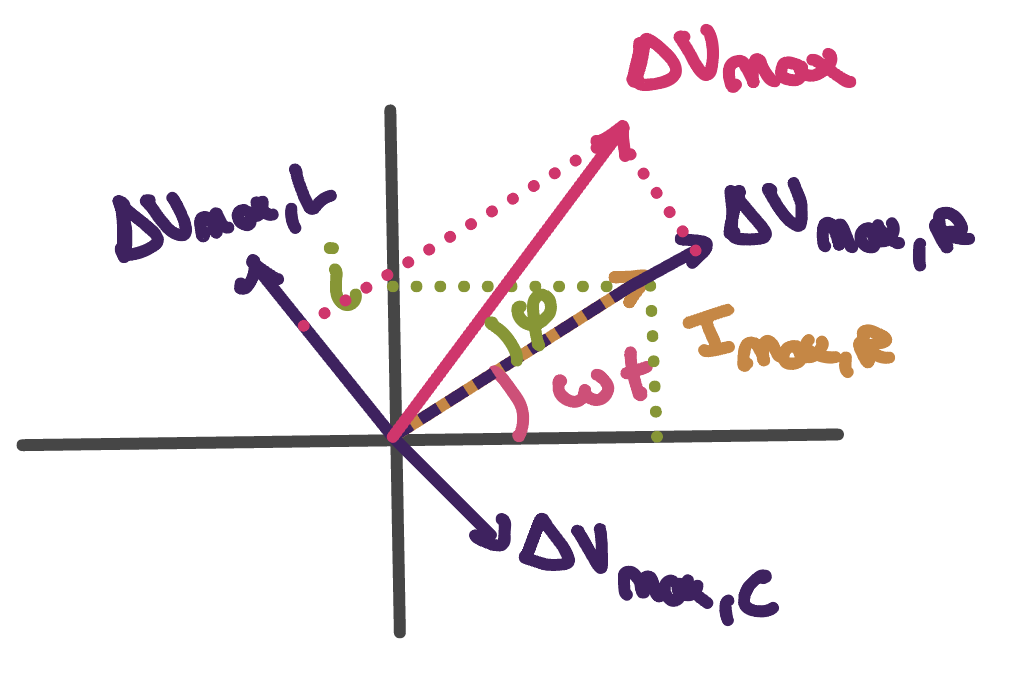
\includegraphics[scale=0.3]{oz09/resources/Oz9Oef1-serie.png}
                \end{center}
                waarbij 
                \begin{equation*}
                    |\Delta V_{\text{max},R}| \approx \frac{3}{2}|\Delta V_{\text{max},L}| \approx 3|\Delta V_{\text{max},C}|.
                \end{equation*}
                We berekenen $Z$ (met Pythagoras):
                \begin{equation*}
                    Z = \sqrt{R^2 + (X_L - X_C)^2} \approx 319 \ \Omega
                \end{equation*}
                We berekenen $\phi$:
                \begin{equation*}
                    \phi = \tan^{-1}\left(\frac{X_L - X_C}{R}\right) \approx 20^\circ
                \end{equation*}
  
            \item Parallelschakeling: $\Delta V$ is gelijk. We hebben het volgende fasor diagram
                \begin{center}
                    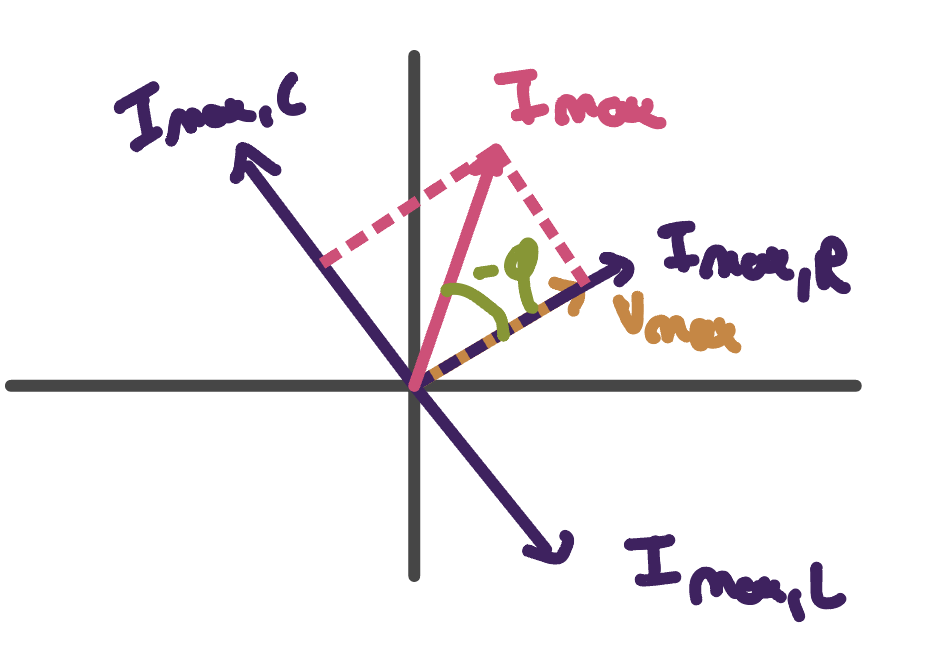
\includegraphics[scale=0.3]{oz09/resources/Oz9Oef1-parallel.png}
                \end{center}
                waarbij
                \begin{equation*}
                    |\Delta I_{\text{max},C}| \approx 2|\Delta I_{\text{max},L}| \approx 3|\Delta I_{\text{max},R}|.
                \end{equation*}
                We berekenen $Z$ (met Pythagoras):
                \begin{equation*}
                    Z = \frac{1}{\sqrt{\frac{1}{R^2} + \left(\frac{1}{X_L} - \frac{1}{X_C}\right)^2}} = 103 \ \Omega
                \end{equation*}
                We berekenen $\phi$:
                \begin{equation*}
                    \phi = \tan^{-1}\left(\frac{\frac{1}{X_L} - \frac{1}{X_R}}{\frac{1}{R}}\right) \approx -61^\circ
                \end{equation*}
        \end{itemize}
\end{description}

\vspace{1cm}

\phantomsection
\label{OZ9:2}
\textbf{\underline{OZ 9 - Wisselstroomkringen - Oefening 2:}}
\vspace{0.5cm}

% \begin{enumerate}[(a)]
%     \item #
% \end{enumerate}

% \begin{description}[labelwidth=1.5cm, leftmargin=!]
%     \item[Geg. :]   
%     \item[Gevr. :] 
%     \item[Opl. :]   
% \end{description}

\vspace{1cm}

\phantomsection
\label{OZ9:3}
\textbf{\underline{OZ 9 - Wisselstroomkringen - Oefening 3:}}
\vspace{0.5cm}

% \begin{enumerate}[(a)]
%     \item #
% \end{enumerate}

% \begin{description}[labelwidth=1.5cm, leftmargin=!]
%     \item[Geg. :]   
%     \item[Gevr. :] 
%     \item[Opl. :]   
% \end{description}

\vspace{1cm}

\phantomsection
\label{OZ9:4}
\textbf{\underline{OZ 9 - Wisselstroomkringen - Oefening 4:}}
\vspace{0.5cm}

In de schakeling in onderstaande figuur, neem aan dat alle parameters behalve C gegeven zijn.

\begin{enumerate}[(a)]
    \item Bepaal de stromen in functie van de tijd indien beide schakelaars gesloten zijn.
    \item Vind het vermogen geleverd aan de schakeling. \vspace{0.3cm} \\ 
\begin{minipage}{.56\textwidth}
    \item Vind de stroom in functie van de tijd na het openen van enkel schakelaar $S_1$.   
    \item Nadat schakelaar $S_2$ ook geopend is, zijn de stroom en de spanning in fase. Vind de capaciteit $C$.
    \item Vind de impedantie van het circuit wanneer beide schakelaars geopend zijn bij deze frequentie.
    \item Vind de maximale energie opgeslagen in de condensator en de spoel tijdens de oscillaties.
    \item De frequentie van de spanningsbron wordt nu verdubbeld. Vind het faseverschil tussen de stroom en de spanning.
    \item Vind de frequentie van de bronspanning die ervoor zorgt dat de inductieve reactantie de helft is van de capacitieve reactantie.
\end{minipage}
\begin{minipage}{.4\textwidth}
   \vspace{-0.5cm}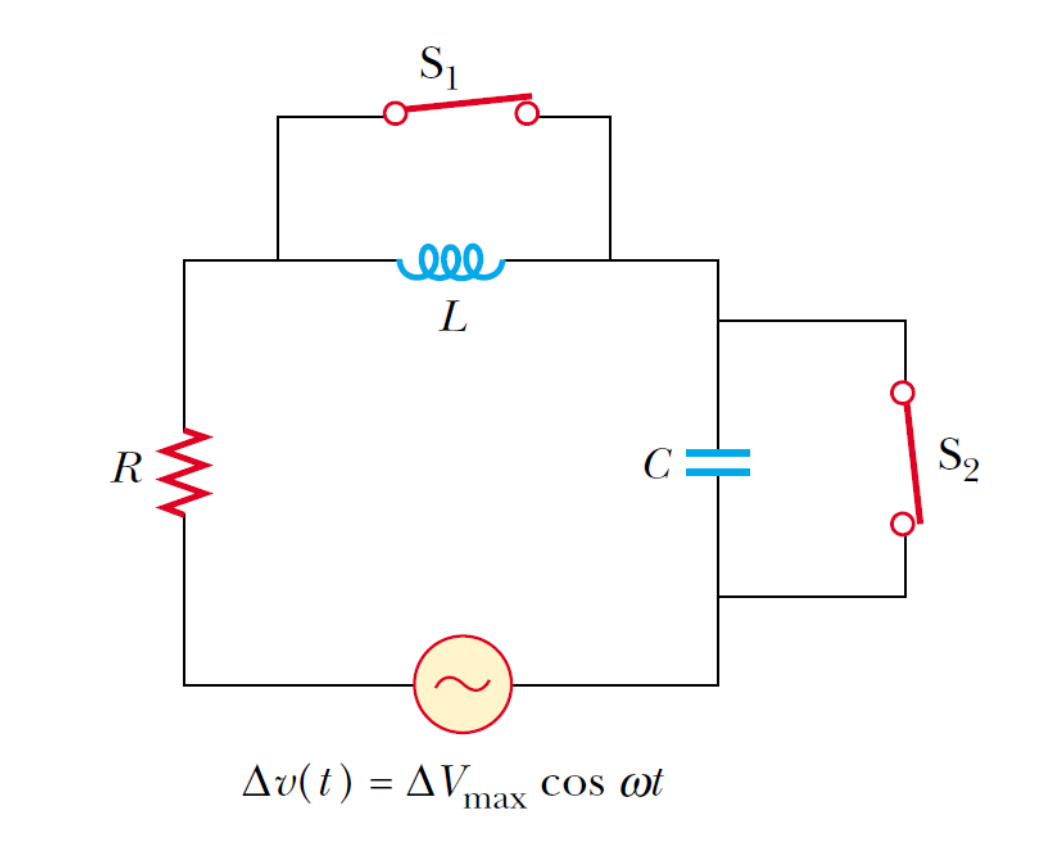
\includegraphics[scale = 0.4]{oz09/resources/Oz9Oef4.png}
\end{minipage}

\end{enumerate}

\begin{description}[labelwidth=1.5cm, leftmargin=!]
    \item[Geg. :]  $R$, $L$, $\Delta v(t) = \Delta V_\text{max} \cos(\omega t)$
\end{description}

\begin{enumerate}[(a)]
    \item 
        \begin{description}[labelwidth=1.5cm, leftmargin=!]
            \item[Geg. :]  $S_1$ en $S_2$ gesloten
            \item[Gevr. :] $i(t)$ ?
            \item[Opl. :]   
                We kunnen a\@.d\@.h\@.v\@. de weerstand een formule voor de stroom afleiden uit $v(t)$, namelijk
                \begin{equation*}
                    i(t) = \frac{\Delta v(t)}{R} = \frac{\Delta V_{\text{max}}}{R} \cos(\omega t)
                \end{equation*}
        \end{description}
    \item
        \begin{description}[labelwidth=1.5cm, leftmargin=!]
            \item[Gevr. :] $P_{\text{gem}}$ ?
            \item[Opl. :]   
                Het gemiddelde vermogen geleverd aan een wisselstroomkring, vinden we met:
                \begin{equation*}
                    P_{\text{gem}} = \frac{1}{2}I_{\text{max}}V_{\text{max}}\cos(\phi).
                \end{equation*}
                Dit kunnen we combineren met het resultaat van (a) waarbij $t = 0 \ \text{s}$ en $\phi = 0^\circ$, vinden we:
                \begin{equation*}
                    P_{\text{gem}} = \frac{1}{2}\frac{(\Delta V_{\text{max}})^2}{R}.
                \end{equation*}
        \end{description}
    \item
        \begin{description}[labelwidth=1.5cm, leftmargin=!]
            \item[Geg. :] $S_1$ open en $S_2$ gesloten
            \item[Gevr. :]  $i(t)$ ?
            \item[Opl. :]   
                We kunnen de stroom afleiden uit $\Delta v(t)$ en de impedantie van het circuit: 
                \begin{equation*}
                    i(t) = \frac{\Delta V_{\text{max}}}{Z} \cos(\omega t + \phi)
                \end{equation*}
                waarbij we moeten rekening houden met $\phi$.
        \end{description}
    \item
        \begin{description}[labelwidth=1.5cm, leftmargin=!]
            \item[Geg. :] $S_1$ open en $S_2$ open, $\phi = 0^\circ$
            \item[Gevr. :] $C$ ?
            \item[Opl. :]   
                Sinds er gegeven is dat de spanning en stroom in fase zijn en dus $\phi = 0$, volgt dat we mogen spreken van resonantie. Er volgt dus uit de resonantiehoeksnelheid:
                \begin{equation*}
                    \omega_0 = \sqrt{\frac{1}{LC}} \ \Rightarrow \ C = \frac{1}{\omega_0^2L}
                \end{equation*}
        \end{description}
    \item
        \begin{description}[labelwidth=1.5cm, leftmargin=!]
            \item[Geg. :]  $S_1$ open en $S_2$ open, $f_0$
            \item[Gevr. :] $Z$ ?
            \item[Opl. :]  
                We spreken hier van resonantie, wat betekent dat $X_L = X_C$, en dus volgt voor de impedantie:
                \begin{equation*}
                    Z = \sqrt{R^2 + (X_L - X_C)^2} = R
                \end{equation*} 
        \end{description}
        \item
        \begin{description}[labelwidth=1.5cm, leftmargin=!]
            \item[Gevr. :] $U_{\text{max}, C}$, $U_{\text{max}, L}$
            \item[Opl. :] 
            \begin{itemize}
                \item $U_{\text{max}, C}$: \\
                    De energie opgeslagen in een condensator werd gegeven door:
                    \begin{equation*}
                        U_{C} = \frac{1}{2}C(\Delta v)^2 = \frac{1}{2}Ci^2X_C^2.
                    \end{equation*}
                    Dit is maximaal als de spanning maximaal, en dus de stroom maximaal is: 
                    \begin{equation*}
                        U_{\text{max}, C} = CI_{\text{max}}^2X_C^2 = \frac{(L\Delta V_{\text{max}})^2}{2R^2}
                    \end{equation*}
                \item $U_{\text{max}, L}$: \\
                    De energie opgeslagen in een inductor werd gegeven door:
                    \begin{equation*}
                        U_{L} = \frac{1}{2}L(I)^2.
                    \end{equation*}
                    Dit is maximaal als de stroom maximaal is:
                    \begin{equation*}
                        U_{\text{max},L} = \frac{1}{2}L(I_{\text{max}})^2 = \frac{(L\Delta V_{\text{max}})^2}{2R^2}.
                    \end{equation*}
            \end{itemize}
        \end{description}
    \item
        \begin{description}[labelwidth=1.5cm, leftmargin=!]
            \item[Geg. :]  $f' = 2f_{0} \ \Rightarrow \ \omega' = 2\omega_0$ 
            \item[Gevr. :] $\phi$ ?
            \item[Opl. :]   
                We berekenen $\phi$ met de geziene formule:
                \begin{align*}
                    \phi 
                        &= \tan^{-1}\left(\frac{X_L-X_C}{R}\right) \\
                        &= \tan^{-1}\left(\frac{\omega' L - \frac{1}{\omega' C}}{R}\right) \\
                        &= \tan^{-1}\left(\frac{2\omega_0 L - \frac{1}{2\omega_0 C}}{R}\right) \\
                        &= \tan^{-1}\left(\frac{\frac{2L}{\sqrt{LC}}L - \frac{\sqrt{LC}}{2C}}{R}\right) \\
                        &= \ldots \\
                        &= \tan^{-1}\left(\frac{3}{2}\sqrt{\frac{L}{C}}\right)
                \end{align*}
        \end{description}
    \item
        \begin{description}[labelwidth=1.5cm, leftmargin=!]
            \item[Geg. :]   $X_L = \frac{1}{2}X_C$
            \item[Gevr. :]  $f'$ ?
            \item[Opl. :]   
                Als de inductieve reactantie de helft is van de capacitieve reactantie, dan volgt: 
                \begin{equation*}
                    \omega = \frac{1}{2\sqrt{LC}} = \frac{\omega_0}{2}
                \end{equation*}
        \end{description}
\end{enumerate}

% \begin{description}[labelwidth=1.5cm, leftmargin=!]
%     \item[Geg. :]   
%     \item[Gevr. :] 
%     \item[Opl. :]   
% \end{description}

\vspace{1cm}

\newpage

\pagebreak

\fakesection{Oefenzitting 10}


\phantomsection
\label{OZ10:1}
% \textbf{\underline{OZ 10 - De vergelijkingen van Maxwell + Herhalingsoefeningen - Oefening 1:}}
% \vspace{0.5cm}

% (\hyperref[OZ2:3]{Oefenzitting 2, oefening 3}) Een cirkelvormige lus met straal $ r $ draagt een stroom $ I $. De lus wordt in een magnetisch veld geplaatst waarvan de rechte veldlijnen lijken te divergeren vanuit een punt dat in het midden onder de lus op een afstand $ d $ ligt. Bepaal de kracht op de lus.

% \vspace{0.5cm}

% \hyperref[OZ2:3]{Klik hier om de uitwerking te bekijken}

% \vspace{1cm}

\newpage

\phantomsection
\label{OZ10:2}
% \textbf{\underline{OZ 10 - De vergelijkingen van Maxwell + Herhalingsoefeningen - Oefening 2:}}
% \vspace{0.5cm}

% (\hyperref[OZ4:3]{Oefenzitting 4, oefening 3}) Een geleider die een stroom $ 2I $ draagt, splitst zich in twee (Figuur 10.1). Elke afgesplitste geleider draagt een stroom $ I $. Bereken de $ y $-component van het magnetische veld in het punt $ P $ als functie van $ \theta $ en $ a $. Ter verduidelijking: $ 2I $ stroomt langs de $ x $-as en splitst in het $ xy $-vlak. $ P $ ligt op de $ z $-as. (Hint: reken eerst $ \vec{B} $ uit in $ P $ van een stuk geleider met lengte $ L $.)

% \begin{figure}[H]
%     \centering
%     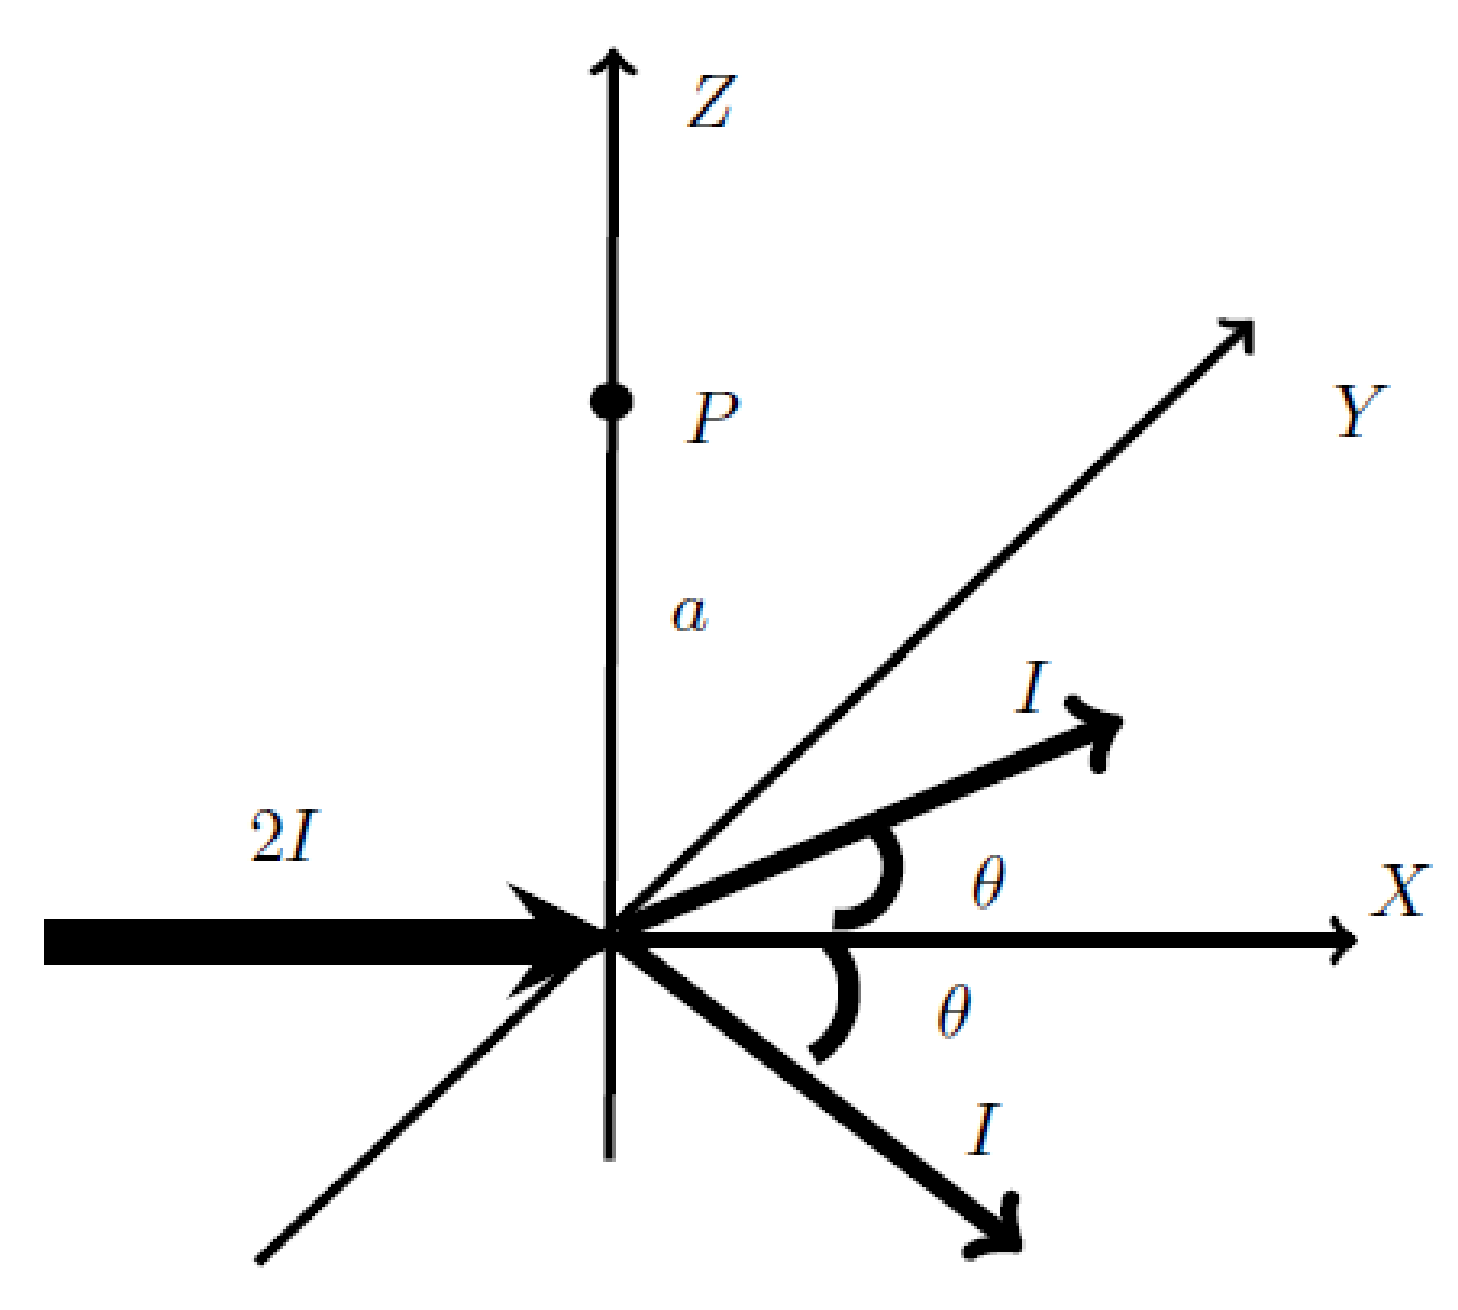
\includegraphics[width=5cm]{oz04/resources/oef-3-opgave.png}
    
%     \textbf{Figuur 10.1}
% \end{figure}

% \hyperref[OZ4:3]{Klik hier om de uitwerking te bekijken}

% \vspace{1cm}

\newpage

\phantomsection
\label{OZ10:3}
% \textbf{\underline{OZ 10 - De vergelijkingen van Maxwell + Herhalingsoefeningen - Oefening 3:}}
% \vspace{0.5cm}

% (\hyperref[OZ9:4]{Oefenzitting 9, oefening 4}) Een weerstand van $ 10,0 \ \Omega $, een spoel met inductantie $ 10,0 $ mH en een condensator van $ 100 \ \mu$F worden in serie aangesloten op een $ 50,0 $ V (rms) spanningsbron met een variabele frequentie. bepaal de energie die de bron levert aan het circuit in één periode als de frequentie wordt ingesteld op het dubbel van de resonantiefrequentie.

% \vspace{0.5cm}

% \hyperref[OZ9:4]{Klik hier om de uitwerking te bekijken}

% \vspace{1cm}

\newpage

\phantomsection
\label{OZ10:4}
\textbf{\underline{OZ 10 - De vergelijkingen van Maxwell - Oefening 4:}}
\vspace{0.5cm}

Een zeer grote parallelle platen condensator draagt een lading met een uniforme lading per eenheid oppervlakte $+\sigma$ op de bovenste plaat en $-\sigma$ op de onderste plaat. Beide platen liggen horizontaal en bewegen horizontaal met een snelheid $v$ naar rechts.

\begin{enumerate}[(a)]
    \item Wat is het magnetisch veld tussen de platen?
    \item Wat is het magnetisch veld in de buurt van de platen, maar buiten de condensator
    \item Wat is de grootte en de richting van de magnetische kracht per eenheid oppervlakte op de bovenste plaat?
    \item Op welke snelheid $v$ zal de magnetische kracht op een plaat gelijk zijn aan de elektrische kracht op die plaat?
\end{enumerate}

\begin{enumerate}[(a)]
    \item 
        \begin{description}[labelwidth=1.5cm, leftmargin=!]
            \item[Geg. :]   
            \item[Gevr. :] 
            \item[Opl. :]   
        \end{description}
    \item 
        \begin{description}[labelwidth=1.5cm, leftmargin=!]
            \item[Geg. :]   
            \item[Gevr. :] 
            \item[Opl. :]   
        \end{description}
    \item 
        \begin{description}[labelwidth=1.5cm, leftmargin=!]
            \item[Geg. :]   
            \item[Gevr. :] 
            \item[Opl. :]   
        \end{description}
    \item 
        \begin{description}[labelwidth=1.5cm, leftmargin=!]
            \item[Geg. :]   
            \item[Gevr. :] 
            \item[Opl. :]   
        \end{description}
\end{enumerate}

% \begin{description}[labelwidth=1.5cm, leftmargin=!]
%     \item[Geg. :]   
%     \item[Gevr. :] 
%     \item[Opl. :]   
% \end{description}

\vspace{1cm}

\newpage

\phantomsection
\label{OZ10:5}
% \textbf{\underline{OZ 10 - De vergelijkingen van Maxwell + Herhalingsoefeningen - Oefening 5:}}
% \vspace{0.5cm}

% Stel een condensator gevormd door cirkelvormige parallele platen met straal $ R $ die op een loodrechte afstand $ d $ van elkaar staan. Stel hierover zet je een potentiaalverschil van $ V(t) = V_0 \left( 1 - e^{-mt} \right) $, met $ m $ een positieve constante en $ t \geq 0 $.

% \begin{enumerate}[(a)]
%     \item Wat zijn de oorzaken van het creëeren van een magnetisch veld tussen de platen?
%     \item Vind de uitdrukking voor het magnetisch veld binnen de condensator. Wanneer is het magnetisch veld maximaal?
%     \item Wat is het magnetisch veld buiten de condensator? Wanneer is deze maximaal?
%     \item Wat gebeurt er als er een diëlectricum wordt ingebracht?
% \end{enumerate}

% \begin{description}[labelwidth=1.5cm, leftmargin=!]
%     \item[Geg. :]   $ V(t) = V_0 \left( 1 - e^{-mt} \right) $
% \end{description}

% \begin{enumerate}[(a)]
%     \item De wet van Ampère-Maxwell
%     \item 
%         \begin{description}[labelwidth=1.5cm, leftmargin=!]
%             \item[Gevr. :]  $ B $;
%             \item[Opl. :]   $  $
%         \end{description}
% \end{enumerate}

% \vspace{1cm}

% \phantomsection
% \label{OZ10:6}
% % \textbf{\underline{OZ 10 - De vergelijkingen van Maxwell + Herhalingsoefeningen - Oefening 6:}}
% \vspace{0.5cm}

% Beschouw een ruimte met elektrische veld $ \vec{E} = \left(80,0 \hat{\imath} + 32,0 \hat{\jmath} - 64,0 \hat{k} \right) $ N/C en magnetisch veld $ \vec{B} = \left(0,200 \hat{\imath} + 0,0800 \hat{\jmath} + 0,290 \hat{k} \right) \ \mu$T.

% \begin{enumerate}[(a)]
%     \item Toon aan dat de twee velden loodrecht op elkaar staan.
%     \item Bepaal de Poynting vector voor deze velden.
% \end{enumerate}

% \begin{description}[labelwidth=1.5cm, leftmargin=!]
%     \item[Geg. :]   $ \vec{E} = \left(80,0 \hat{\imath} + 32,0 \hat{\jmath} - 64,0 \hat{k} \right) $ N/C; $ \vec{B} = \left(0,200 \hat{\imath} + 0,0800 \hat{\jmath} + 0,290 \hat{k} \right) \ \mu$T;
% \end{description}

% \begin{enumerate}[(a)]
%     \item
%         \begin{description}[labelwidth=1.5cm, leftmargin=!]
%             \item[Gevr. :]  Toon aan dat $ \vec{E} $ en $ \vec{B} $ loodrecht op elkaar staan;
%             \item[Opl. :]   $ \vec{E} \cdot \vec{B} = \left(80,0 \hat{\imath} + 32,0 \hat{\jmath} - 64,0 \hat{k} \right) \cdot \left(0,200 \hat{\imath} + 0,0800 \hat{\jmath} + 0,290 \hat{k} \right) $
            
%                             \hspace{0.8cm} $ 
%                             = 80,0 \cdot 0,200 + 32,0 \cdot 0,0800 + (-64,0) \cdot 0,290 
%                             = 0 $
%         \end{description}
%     \item
%         \begin{description}[labelwidth=1.5cm, leftmargin=!]
%             \item[Gevr. :]  $ \vec{S} $;
%             \item[Opl. :]   $ \vec{S} = \dfrac{1}{\mu_0} \vec{E} \times \vec{B}
%                             = \dfrac{1}{4\pi \cdot 10^{-7}} \left(80,0 \hat{\imath} + 32,0 \hat{\jmath} - 64,0 \hat{k} \right) \times \left(0,200 \hat{\imath} + 0,0800 \hat{\jmath} + 0,290 \hat{k} \right) \cdot 10^{-6} $
                            
%                             \hspace{0.23cm} $ 
%                             = \dfrac{1}{4\pi \cdot 10^{-1}} ( \left( 32,0 \cdot 0,290 - (-64,0) \cdot 0,0800 \right) \hat{\imath} $
                            
%                             \hspace{2.5cm} $ + \left( (-64,0) \cdot 0,200 - 80,0 \cdot 0,290 \right) \hat{\jmath} $
                            
%                             \hspace{2.5cm} $ + \left( 80,0 \cdot 0,0800 - 32,0 \cdot 0,200 \right) \hat{k} ) $
                            
%                             \hspace{0.23cm} $ 
%                             = \dfrac{1}{4\pi \cdot 10^{-1}} \left( 14,4 \hat{\imath} - 36 \hat{\jmath} + 0 \hat{k} \right) $
                            
%                             \hspace{0.23cm} $ 
%                             = \left( 11,4591559026 \hat{\imath} - 28,6478897565 \hat{\jmath} \right) $ W/m$ ^2 $
                            
                            
                            
%                             \hspace{0.23cm} $ 
%                             \approx \left( 11,5 \hat{\imath} - 28,6 \hat{\jmath} \right) $ W/m$ ^2 $
%         \end{description}
% \end{enumerate}

\newpage

\end{document} 